% Chapitre « données, décalage de domaine et démonstration » (contribution de Yosra), à inclure dans le rapport
% (classe report) par % Chapitre « données, décalage de domaine et démonstration » (contribution de Yosra), à inclure dans le rapport
% (classe report) par % Chapitre « données, décalage de domaine et démonstration » (contribution de Yosra), à inclure dans le rapport
% (classe report) par % Chapitre « données, décalage de domaine et démonstration » (contribution de Yosra), à inclure dans le rapport
% (classe report) par \input{docs/rapport/chapitre_yosra}. Version LaTeX de docs/pipeline/RAPPORT.md (commit 4540d85) :
% plan, contenu et formulations conservés ; chemins des fichiers sources ajoutés pour chaque chiffre.
% Paquets attendus dans le préambule : babel (french), graphicx, booktabs, makecell, hyperref, float.
% Réglages à mettre dans le préambule du rapport final :
%   \addto\captionsfrench{\def\tablename{Tableau}}   % « Tableau » au lieu de « Table »
%   \hypersetup{hidelinks}                             % liens sans cadre rouge
% Les chemins des figures sont relatifs à la racine du dépôt.
% Statut d'origine (RAPPORT.md) : brouillon scientifique fondé sur les résultats locaux disponibles ; les valeurs
% finales doivent être prises dans les JSON/CSV générés après le dernier QC ; les expériences sans prédictions ou
% checkpoints ne sont pas présentées comme réalisées.

% Chemins de fichiers longs : coupures de ligne aussi permises après « _ » et « - » dans \nolinkurl et \url.
\makeatletter
\g@addto@macro\UrlBreaks{\do\_\do\-}
\makeatother
% Étirement d'urgence limité à ce chapitre (lignes chargées de chemins), remis à zéro à la fin.
\setlength{\emergencystretch}{3em}

\chapter{Données, décalage de domaine et démonstration}
\label{chap:yosra}

\section{Introduction et questions de recherche}
\label{sec:yosra-introduction}

Ce projet étudie la segmentation des lésions d'AVC sur des IRM T1 acquises dans plusieurs centres.
Les différences de scanner, protocole et résolution peuvent modifier la distribution des images.
Notre objectif est de mesurer ce décalage, d'évaluer la généralisation des modèles sur des centres absents de l'entraînement, puis d'étudier la possibilité d'anticiper et de réduire leur perte de performance.

Trois questions structurent le projet : quel est l'écart entre test ID et test OOD ?
Les architectures Transformer améliorent-elles la généralisation par rapport à nnU-Net ?
Quelles techniques de généralisation ou d'adaptation réduisent cet écart ?
La contribution de Yosra fournit le pipeline de données, les partitions communes, les mesures du décalage, les analyses explicatives et l'interface de démonstration.
Les comparaisons de segmentation et l'adaptation continue sont produites par Fayfa et Anas.

\section{Données et contrôle qualité}
\label{sec:yosra-donnees}

L'inventaire local contient 1\,453 paires IRM/masque dans 55 centres.
Le centre R032, soit 37 cas, est exclu provisoirement pour espacement incohérent.
Les métadonnées vides sont signalées sans supprimer une paire utilisable.
Les masques vides sont conservés comme cas négatifs.
Le délai post-AVC reste numérique ; \texttt{CHRONICITY}, codé 1/vide, n'est pas interprété comme une catégorie aigu/subaigu/chronique
(\nolinkurl{analysis/reports/qc_by_center/summary.json}, \nolinkurl{analysis/reports/qc_by_center/exclusion_reasons.csv}).

La livraison v2 contient 1\,415 volumes prétraités, relus et exportés.
Elle exclut les 37 cas R032 et met un cas supplémentaire en quarantaine technique.
Le split v1 est archivé ; v2 retire uniquement ce cas, sans déplacer les autres sujets ni les centres.
La relecture collective de cette quarantaine reste nécessaire ; les annotations brutes sont intactes
(\nolinkurl{preprocessing/reports/release_v2.json}, \nolinkurl{preprocessing/qc_exclusions.json}).

\section{Pipeline Spark}
\label{sec:yosra-pipeline}

Chaque sujet constitue une unité de travail.
Le pipeline réoriente les images en RAS, rééchantillonne à 1~mm isotrope (linéaire pour l'image, plus proche voisin pour les masques), normalise les intensités dans le support cérébral et recadre avec une marge de cinq voxels.
Le support est défini par les intensités supérieures à la valeur de fond estimée ; cette précaution traite notamment le centre R029 dont le fond n'est pas nul.
Cette heuristique reste une limite et doit être examinée sur les cas atypiques.

Le z-score est stocké en \texttt{int16} avec un pas de 0,001.
L'erreur d'arrondi est au plus 0,0005 unité de z-score.
Le validateur utilise cette borne, avec une petite marge numérique, pour la moyenne et l'écart-type ; le fond doit rester exactement nul.
Une signature des entrées et paramètres permet la reprise et chaque paire est accompagnée d'un QC (\nolinkurl{preprocessing/week4.py}).

La boîte de recadrage est déterminée par l'image seule.
Le code existant tolère la suppression de labels hors boîte jusqu'à 1~\% du volume lésionnel.
Ce choix n'est pas une correction clinique des annotations : il doit être documenté et validé.
Le dernier cas dépasse cette tolérance (1,76~\% : 77 voxels sur 4\,376, \nolinkurl{preprocessing/qc_exclusions.json}) et est mis en quarantaine dans v2.
L'option N4 a été ajoutée pour une expérience distincte ; elle n'a pas été appliquée au jeu de référence et aucun bénéfice n'en est revendiqué.

\section{Partitions et absence de fuite}
\label{sec:yosra-partitions}

Le fichier commun \nolinkurl{splits.json} version 2 fixe 916 cas d'entraînement/validation, 231 cas ID et 268 cas OOD (\nolinkurl{preprocessing/reports/release_v2.json}).
Six centres OOD sont intégralement retirés : R008, R028, R031, R034, R053 et SOOP.
Les cinq plis séparent les centres d'entraînement et de validation.
Le test ID de chaque pli est limité aux centres présents dans son entraînement.
Le découpage compte 231 sujets ID au total ; pour le pli~0, le test ID n'en garde que 185, car les 46 autres appartiennent aux centres de validation de ce pli, absents de son entraînement (\nolinkurl{splits.json}, \texttt{folds[0].id\_test}).

La sélection des centres OOD varie taille et distance d'intensité.
Comme la distance participe à cette sélection, un écart de distance ID/OOD n'est pas une découverte indépendante.
Les mesures prédictives doivent utiliser la référence d'entraînement du modèle considéré, pas le pool global.
Aucun hyperparamètre d'alerte ne doit être choisi sur le test OOD.

\section{Benchmark}
\label{sec:yosra-benchmark}

Le pilote existant porte sur huit petits volumes et un essai par configuration.
Les temps de calcul sont 56,59~s, 41,46~s, 27,63~s et 42,54~s pour 1, 2, 4 et 8 workers.
L'accélération maximale mesurée est $\times$2,05 avec quatre workers (\nolinkurl{preprocessing/reports/benchmark_summary.csv}, \nolinkurl{preprocessing/reports/benchmark_scope.json}).
La dégradation à huit workers est compatible avec des coûts de concurrence et de ressources ; ce pilote ne permet pas d'en isoler la cause.
Les workers ne constituent pas des cœurs physiques réservés.
Le démarrage Spark n'entre pas dans \texttt{compute\_seconds}.
Les courbes ne sont pas extrapolées au dataset entier.
La figure~\ref{fig:yosra-benchmark} montre l'accélération mesurée.

\begin{figure}[htbp]
  \centering
  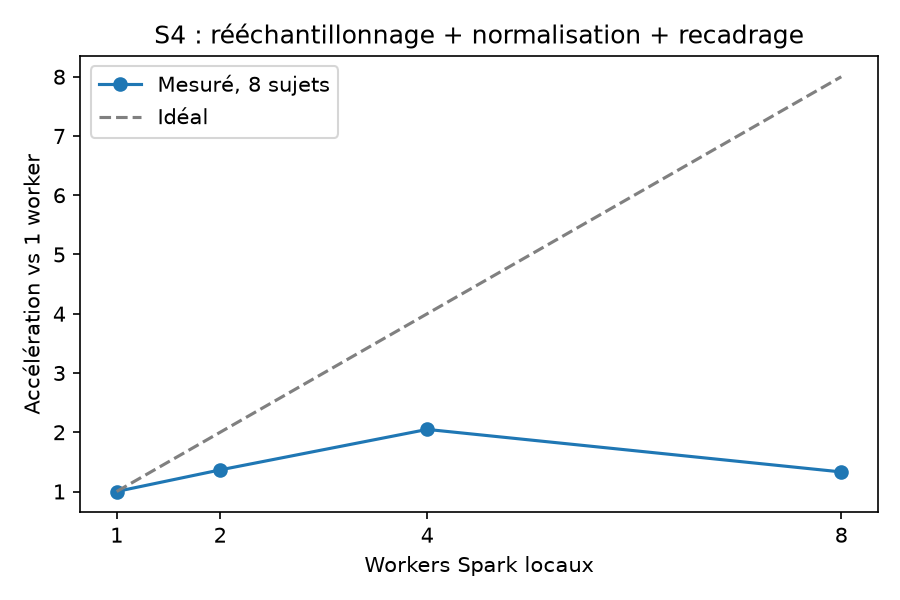
\includegraphics[width=0.6\linewidth]{preprocessing/reports/benchmark_speedup.png}
  \caption{Accélération du prétraitement S4 selon le nombre de workers Spark locaux (8 sujets, un essai).}
  \label{fig:yosra-benchmark}
\end{figure}

\section{Statistiques et empreinte du centre}
\label{sec:yosra-s5-s6}

Les rapports S5 comparent les distributions avant/après prétraitement et mesurent les distances Wasserstein et MMD entre centres et référence.
Le z-score contraint moyenne et variance par scan ; les différences restantes portent donc surtout sur la forme des distributions.
Les échelles avant/après ne sont pas identiques : leur comparaison normalisée reste descriptive.

Le test S6 prédit le centre depuis des histogrammes ou statistiques, avec cinq plis stratifiés, exactitude équilibrée et contrôle à labels mélangés.
Comparer des histogrammes de granularité proche et les mêmes patients permet de mieux isoler l'effet du prétraitement.
Une empreinte reconnaissable n'implique pas à elle seule une baisse du Dice.

Valeurs et figures : \nolinkurl{analysis/reports/post_stats_summary.json}, \nolinkurl{analysis/reports/site_fingerprint_s6.csv}, figures~\ref{fig:yosra-s5-avant-apres}, \ref{fig:yosra-s5-distances} et~\ref{fig:yosra-s6}.
Les versions historiques sur 1\,402 cas ne doivent pas être confondues avec la relance sur 1\,415.
Les versions historiques sur 1\,402 cas sont conservées dans l'historique Git du dépôt
(commit \texttt{5a86471}, fichier \texttt{analysis/reports/post\_stats\_summary.json}).

La relance du 11 novembre couvre 1\,415 sujets dans 54 centres.
La distance relative médiane passe de 0,1315 avant à 0,0376 après, sur la même cohorte disponible.
La corrélation entre Wasserstein et MMD vaut 0,842 pour les centres d'au moins cinq scans.
La médiane de Wasserstein vaut 0,0376 pour ID et 0,0900 pour OOD ; cet écart reste affecté par la sélection initiale des centres (\nolinkurl{analysis/reports/post_stats_summary.json}).
Le test S6 retient 1\,140 scans de 25 centres.
Avec les histogrammes 32 classes avant / 30 classes après et le meilleur des deux classifieurs, l'exactitude équilibrée vaut 69,7~\% puis 48,9~\%.
Le contrôle mélangé vaut 4,0~\%, proche du hasard à 4~\% (\nolinkurl{analysis/reports/site_fingerprint_s6.csv}, \nolinkurl{analysis/reports/site_fingerprint_s6_summary.json}).
Ces chiffres ne mesurent pas la performance de segmentation.

\begin{figure}[p]
  \centering
  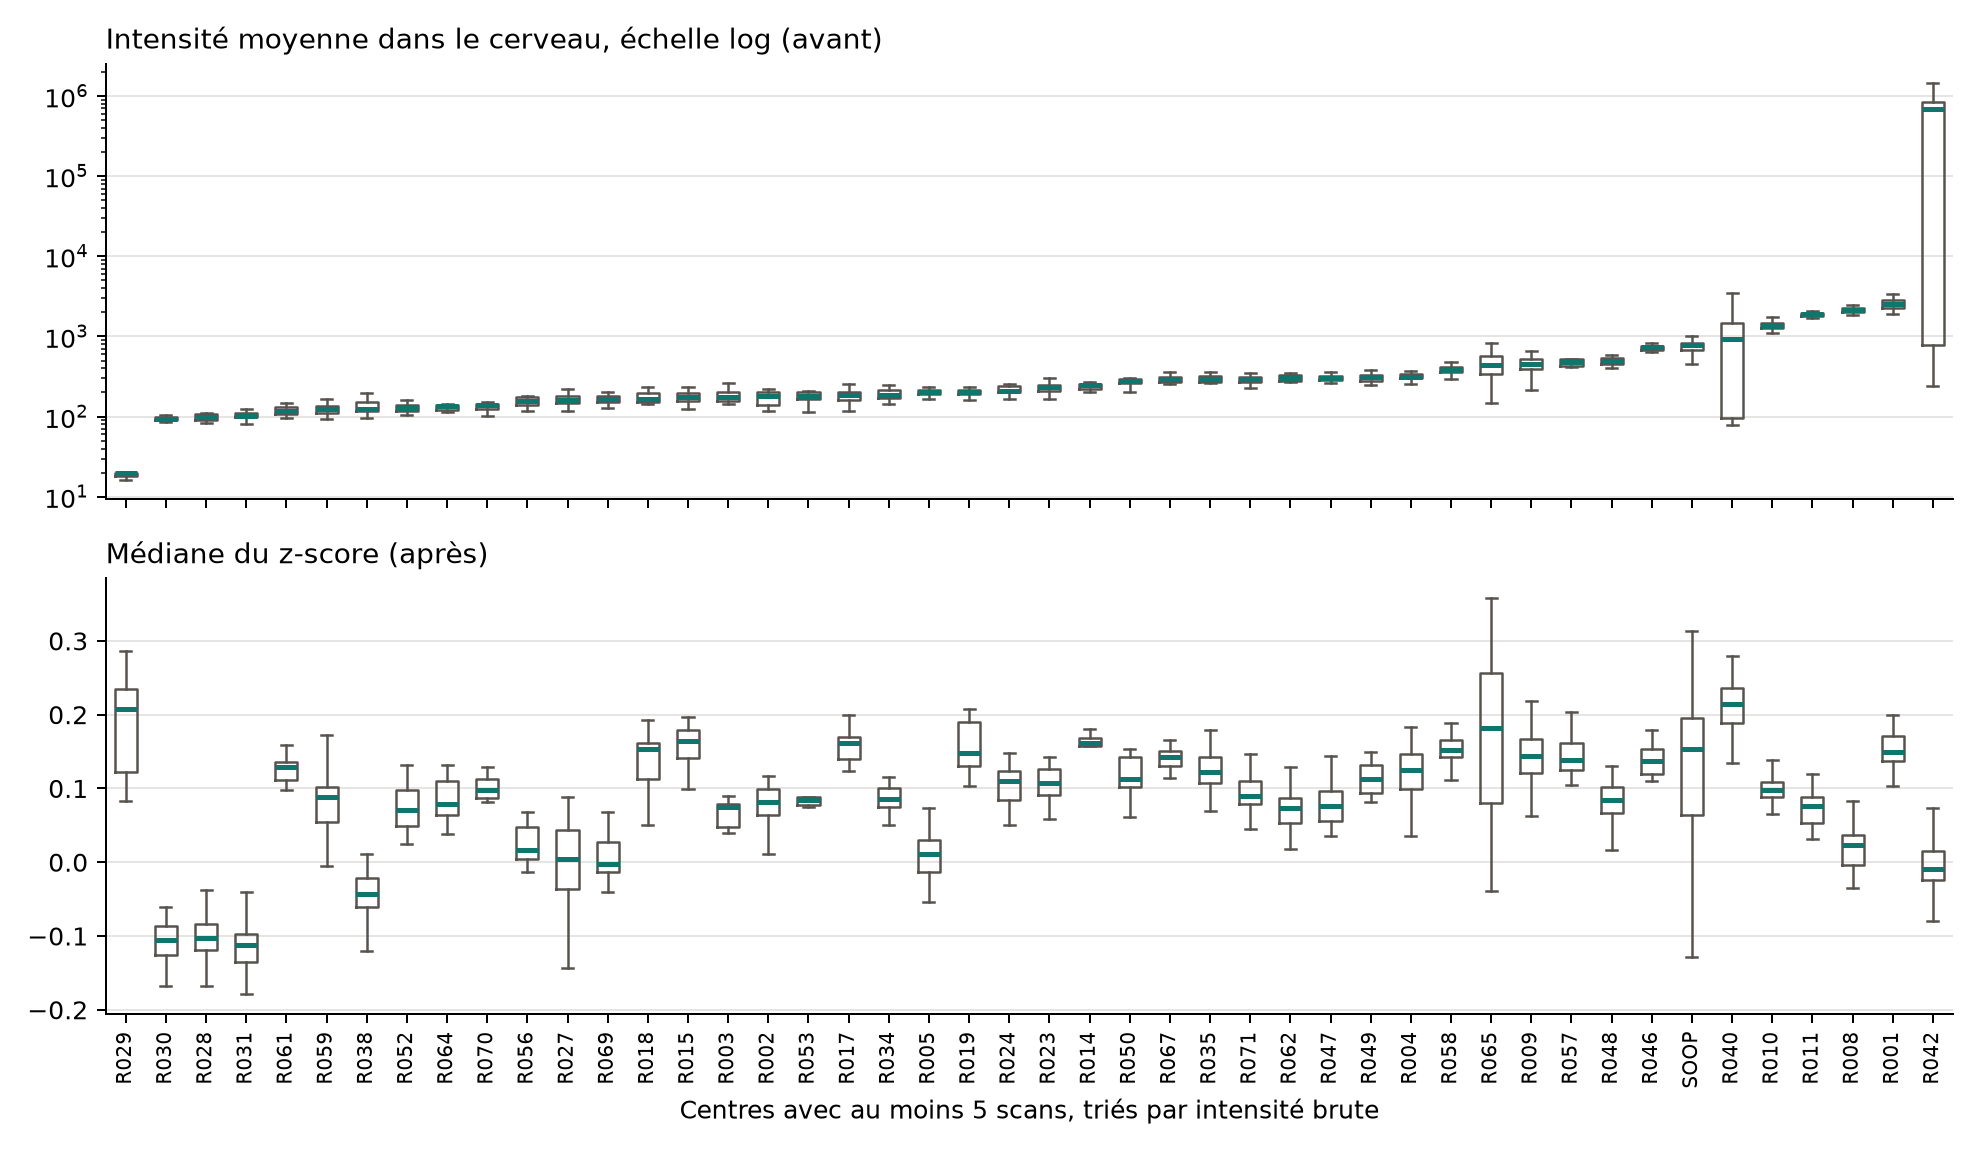
\includegraphics[angle=90,height=0.9\textheight]{figures/s5_avant_apres_par_centre.png}
  \caption{Intensité moyenne dans le cerveau avant prétraitement (échelle log) et médiane du z-score après, par centre (centres d'au moins 5 scans).}
  \label{fig:yosra-s5-avant-apres}
\end{figure}

\begin{figure}[htbp]
  \centering
  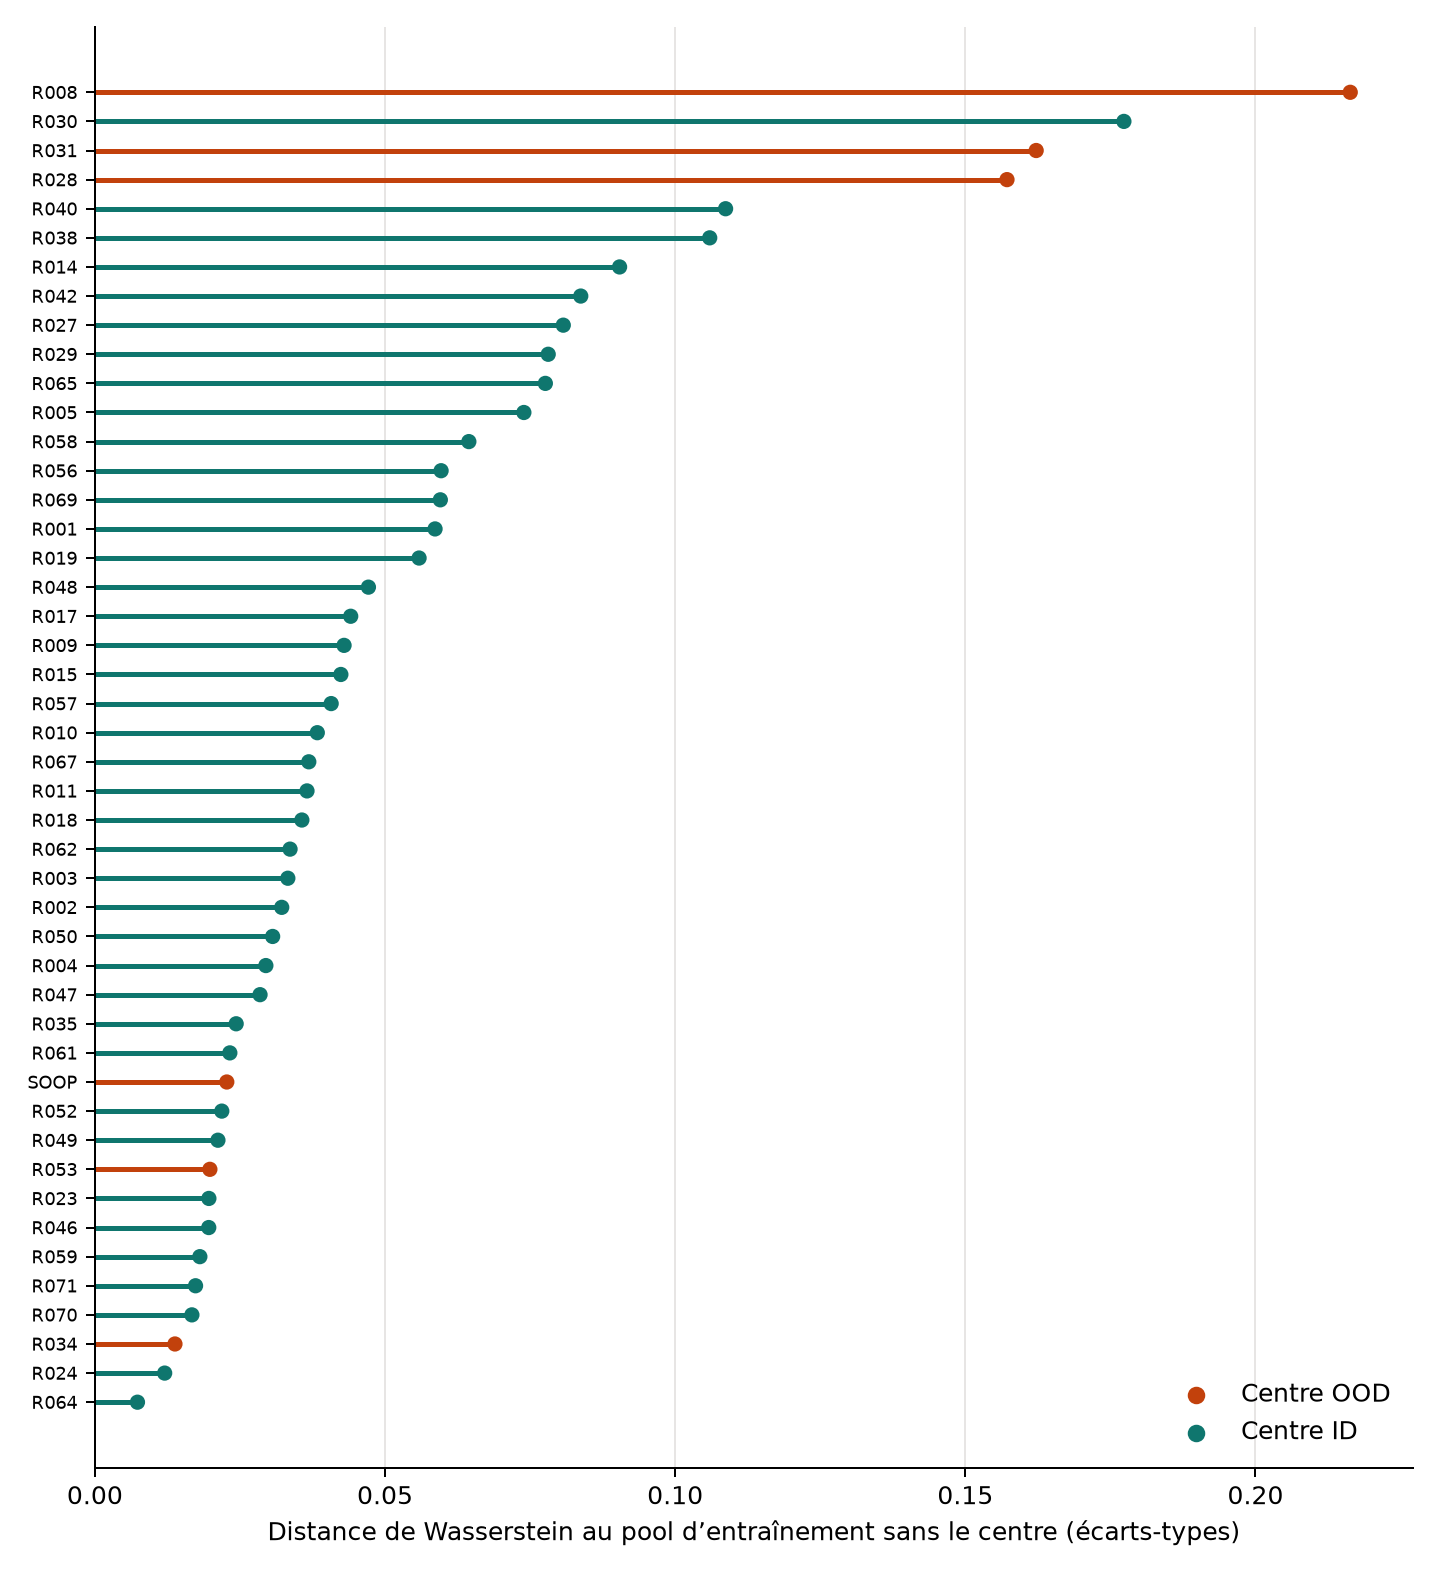
\includegraphics[width=0.85\linewidth]{figures/s5_distances_centres.png}
  \caption{Distance de Wasserstein de chaque centre au pool d'entraînement sans ce centre ; centres OOD en orange.}
  \label{fig:yosra-s5-distances}
\end{figure}

\begin{figure}[htbp]
  \centering
  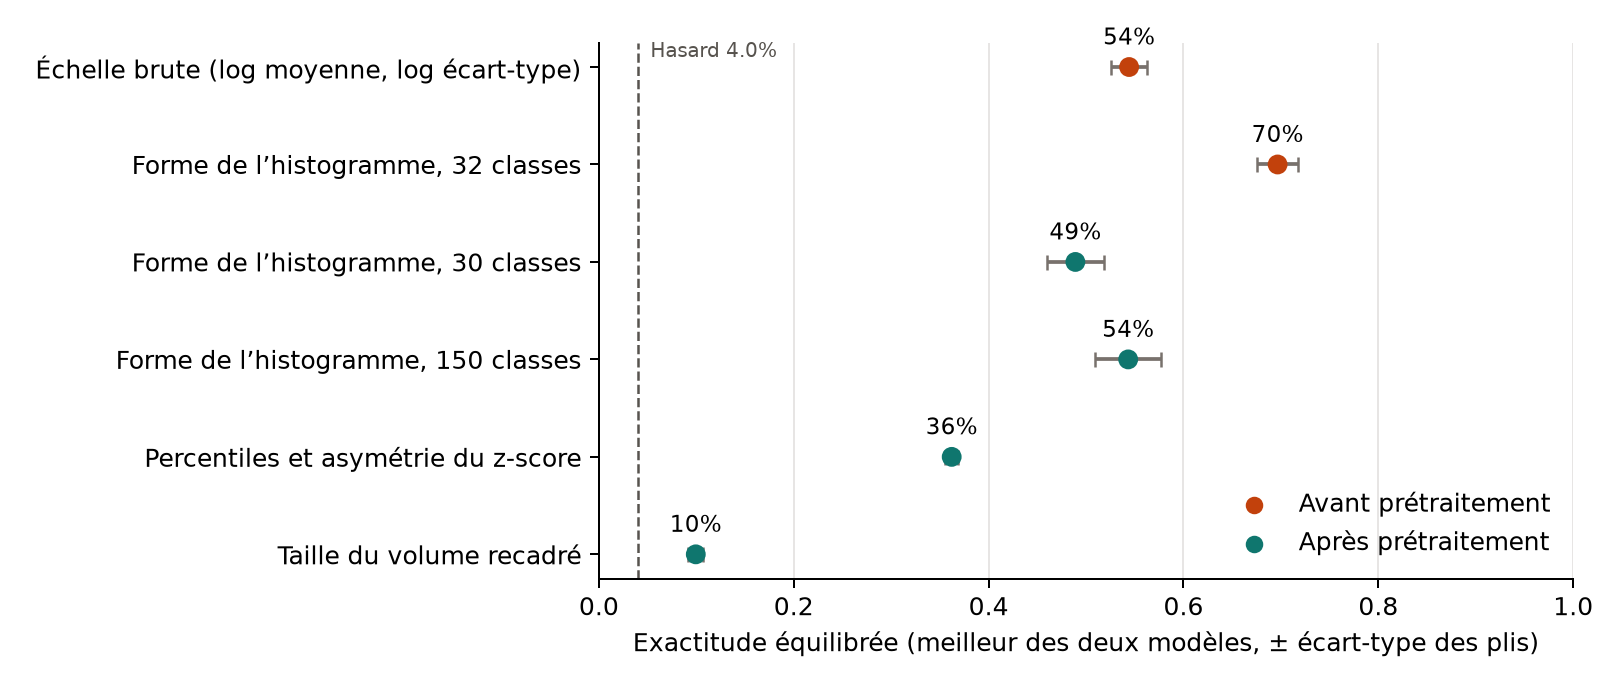
\includegraphics[width=\linewidth]{figures/s6_empreinte_centre.png}
  \caption{Empreinte du centre (S6) : exactitude équilibrée de la prédiction du centre selon la représentation, avant et après prétraitement (hasard : 4~\%).}
  \label{fig:yosra-s6}
\end{figure}

\section{Prédiction d'échec et effet du temps : protocole C1 préparé}
\label{sec:yosra-s7-s8}

S7 met en relation la distance au train du pli et l'erreur $1 - \mathrm{Dice}$ par centre.
Une validation leave-one-center-out produit des prédictions hors calibration.
La régression et le seuil d'alerte sont ajustés uniquement sur les autres centres de validation.
La différence de Dice par rapport au test ID est rapportée séparément.
Sans les résultats C3 de C1, ni corrélation empirique ni performance d'alerte ne peuvent être annoncées.

S8 compare les associations du centre et du délai post-AVC par modèles linéaires emboîtés sur les mêmes cas complets.
Le délai est transformé par $\log(1 + \textrm{jours})$.
Le test de permutation préserve le centre.
Les délais manquants, la sélection des cas et les confusions possibles limitent l'interprétation.
Le protocole n'établit pas une relation causale.

\section{Caractéristiques du réseau (C6 v2)}
\label{sec:yosra-c6}

La version C6 v2 mesure le décalage dans l'espace appris par le réseau plutôt que sur les
intensités. Le modèle C8 (U-Net 3D, augmentation d'intensité, pli 0) est gelé et utilisé en
mode évaluation, sans gradient et sans masque lésionnel. Pour chaque sujet, la sortie du
bottleneck, la couche que lit le classifieur de centre de DANN, est moyennée dans l'espace :
on obtient un vecteur de 320 valeurs par scan.
L'entrée est le volume C1 complet, complété par des zéros jusqu'à un multiple de 16. Le réseau
a été entraîné sur des patchs $96^3$ : sur le volume entier, les normalisations d'instance
portent sur une autre étendue. La même règle est appliquée à tous les scans, ce qui garde la
comparaison entre centres cohérente.

La comparaison d'empreinte baseline / augmentation / DANN demande les checkpoints baseline et
DANN du même protocole ; elle reste à faire.

\section{Démonstration et limites}
\label{sec:yosra-demo}

L'application Gradio affiche les coupes d'une IRM et un masque, calcule le volume lésionnel en mL et accepte une carte d'incertitude.
Un adaptateur permet de brancher le modèle final.
NiiVue fournit une vue 3D locale sur la route \texttt{/viewer/} du même serveur.
ANTsPy peut recaler un template MNI et transférer un atlas de labels ; une inspection visuelle demeure nécessaire avant de nommer les régions.

L'alerte individuelle d'intensité utilise un quantile de validation distinct du seuil par centre.
Elle n'est ni une garantie de performance ni une décision clinique.
En l'absence d'une entrée requise, l'application indique ce qui manque au lieu de créer un résultat.
Le support animé de secours est synthétique et explicitement étiqueté.

\subsection{Interface web du projet}
\label{sec:yosra-frontend}

Une application web (\texttt{frontend/}) présente l'ensemble du projet en dix pages :
vue d'ensemble, avancement du pipeline, contrôle qualité, prétraitement Spark, décalage entre
centres, modèles et Dice, adaptation de domaine, démonstration IRM avec vue 3D, conclusions
et galerie des figures. Le serveur FastAPI lit uniquement les rapports versionnés du dépôt
(\texttt{analysis/reports}, \texttt{preprocessing/reports}, \texttt{baselines/outputs},
\texttt{adaptation/outputs}, \texttt{integration/reports}) : aucun chiffre n'est simulé, et une
expérience absente est signalée comme telle. Chaque page et chaque carte indiquent qui a
produit le résultat. L'interface fonctionne sans étape de construction ni ressource externe ;
seules les figures des dossiers de résultats sont servies, jamais les données IRM. Sept tests
couvrent l'API (\texttt{frontend/tests/test\_server.py}).

\subsection{Branchement du modèle C8}
\label{sec:yosra-c8}

La démonstration (\texttt{demo/app.py}) et l'interface web appellent la fonction désignée par
la variable \texttt{AVC\_PREDICT\_ADAPTER}, au format \texttt{module:fonction}. L'adaptateur de
l'équipe, \texttt{adaptation.demo\_adapter:predict}, applique le prétraitement S4 puis le modèle
retenu (augmentation d'intensité, pli 0) et enregistre le masque en NIfTI \texttt{uint8} dans la
grille de l'IRM reçue. Il demande PyTorch et MONAI, absents de l'environnement de la
démonstration. Le pont \texttt{demo/c8\_bridge.py} lance donc cet adaptateur dans
l'environnement du modèle, dans un processus séparé, et récupère le masque ; la démonstration
utilise \texttt{AVC\_PREDICT\_ADAPTER=c8\_bridge:predict}. Le checkpoint est lu dans
\texttt{data/modeles/unet3d\_intensity\_pli0\_best.pt} (SHA-256 \texttt{ee6b93af\ldots abb6}),
hors du dépôt.

Sur le sujet OOD R034\_sub-r034s003\_ses-1, le rapport de la démonstration donne un volume
lésionnel de 27,058~mL (27\,058 voxels de 1~mm$^3$). Cette valeur concorde avec le volume
prédit lors de l'évaluation du modèle : 27,054~mL dans le fichier \texttt{resultats\_ood\_test.csv}
de la run intensité, conservé hors du dépôt. Sur le sujet OOD R031\_sub-r031s006\_ses-1, envoyé
sans masque à l'interface web, le modèle prédit 33,8~mL pour 27,7~mL annotés, soit un Dice de
0,745, en environ 35~s sur processeur. Ces deux cas vérifient le branchement ; ils ne constituent
pas une évaluation. Le modèle ne produit pas de carte d'incertitude. Cinq tests couvrent les
erreurs du pont (\texttt{tests/test\_c8\_bridge.py}).

\section{Discussion et travaux à terminer}
\label{sec:yosra-discussion}

Les principales limites actuelles sont la quarantaine QC à relire collectivement, le faible nombre de centres pour calibrer un prédicteur d'échec, la dépendance des distances aux effectifs, les métadonnées manquantes et l'absence locale des checkpoints et des Dice correspondant à C1 v2.
Les résultats RQ3 du pli 0 et le checkpoint C8 sont désormais disponibles (chapitre RQ3,
conclusion). Les analyses S7 et S8 sur C1 v2 attendent encore les Dice par sujet, y compris
sur la validation, qui sert à calibrer le seuil d'alerte sans consulter le test. L'empreinte
avant/après DANN attend les checkpoints baseline et DANN. La vidéo de vraie inférence et la
relecture collective restent à faire.
Une analyse S8 historique distincte est disponible plus bas (section~\ref{sec:yosra-s8-historique}).
Les références bibliographiques du document de projet doivent être vérifiées dans leurs publications originales avant d'être reprises dans la version remise.

\section{Compléments vérifiés de la livraison v2}
\label{sec:yosra-livraison}

L'export nnU-Net contient 916 images et labels d'entraînement, 499 images de test (231 ID, 268 OOD) et cinq plis (\nolinkurl{preprocessing/reports/export_v2.json}).
Le contrôle officiel nnU-Net reste à lancer dans l'environnement d'entraînement de Fayfa.
Les autres appartenances de v1 sont conservées.

L'analyse descriptive S8 trouve 1\,073 délais utilisables et 342 manquants ou invalides ; le délai médian est de 365 jours.
Huit centres n'ont aucun délai utilisable.
L'association centre / log-délai (eta carré 0,7475) souligne la nécessité de tenir compte du centre ; elle ne mesure pas l'effet du délai sur le Dice.
Voir \nolinkurl{analysis/reports/s8_metadata/} (\nolinkurl{summary.json}).

Le seuil individuel d'atypie du pli~0 vaut 0,114885 : référence de 733 scans du train, quantile 95~\% sur 183 scans de validation.
Aucun test ID/OOD n'a servi à ce réglage.
Le seuil est enregistré dans \texttt{data/demo/reference\_ood.json} (pli 0, quantile 0,95,
733 scans d'entraînement, 183 de validation), hors du dépôt comme l'ensemble de \texttt{data/}.

Chrome a chargé l'application, produit le rapport synthétique de 2,091~mL, puis affiché les coupes et le rendu 3D NiiVue sans erreur JavaScript (\nolinkurl{docs/pipeline/demo_verification/browser_report.json}).
L'image Docker a été construite et ses routes ainsi que le calcul du rapport ont été testés (\nolinkurl{docs/pipeline/verification.json}).
La vidéo de secours MP4 utilise ces captures réelles d'interface sur un phantom explicitement synthétique ; elle ne montre pas une inférence du réseau.

L'atlas Harvard-Oxford et le template compatible MNI152NLin6Asym ont été récupérés avec leurs sources et empreintes dans \nolinkurl{data/demo/atlas/provenance.json} (hors du dépôt ; copie versionnée : \nolinkurl{docs/pipeline/demo_verification/atlas_provenance.json}).
Les labels corticaux sont prioritaires, puis les labels sous-corticaux décalés de 100 ; les zones non couvertes gardent la valeur zéro.
Le recalage natif exige une relecture anatomique.
Sources : Nilearn Harvard-Oxford\footnote{\url{https://nilearn.github.io/stable/modules/generated/nilearn.datasets.fetch_atlas_harvard_oxford.html}} et TemplateFlow MNI152NLin6Asym\footnote{\url{https://github.com/templateflow/tpl-MNI152NLin6Asym}}.

Le recalage SyN sur l'exemple réel a été exécuté.
Atlas et IRM ont la même grille, les labels restent entiers et 97,75~\% des voxels atlas non nuls se trouvent dans le support d'intensité de l'image (\nolinkurl{docs/pipeline/verification.json}).
La planche locale \nolinkurl{data/demo/registration/qc_overlay.png} (hors du dépôt) a été examinée dans trois plans ; cela ne remplace pas une relecture anatomique experte.
Le rapport régional utilise le masque de référence fourni, sans inférence de réseau.

\section{S8 : résultat exploratoire sur les baselines récupérées}
\label{sec:yosra-s8-historique}

Le 12 novembre, les scores historiques de \texttt{cnn\_pretrained\_freeze-none} ont été rattachés à leur propre partition (903 train, 226 ID validation, 287 OOD), sans les reclasser dans C1 v2.
L'analyse utilise 167 cas ID complets de 31 centres et 257 cas OOD de 12 centres.
En ID, 58 délais manquent ou sont invalides et un Dice est absent ; en OOD, 30 délais manquent ou sont invalides.
Le Dice absent du cas à masque vide n'est pas remplacé par un score supposé.

Après ajustement sur le centre, l'ajout de $\log(1 + \textrm{délai})$ augmente le R$^2$ de 0,000046 en ID ($p$ exploratoire $= 0{,}911$) et de 0,03808 en OOD ($p = 0{,}001$ ; 999 permutations intra-centre pour chaque groupe).
Après ajout de $\log(1 + \textrm{volume lésionnel})$, ces gains sont respectivement 0,000711 et 0,000217 (\nolinkurl{analysis/reports/s8_historical/summary.json}).
L'association OOD dépend donc fortement des variables prises en compte ; elle ne permet pas d'attribuer un effet causal au temps.
Le volume est une analyse de sensibilité, pas un ajustement causal validé.
La figure~\ref{fig:yosra-s8} montre les cas utilisés.

\begin{figure}[htbp]
  \centering
  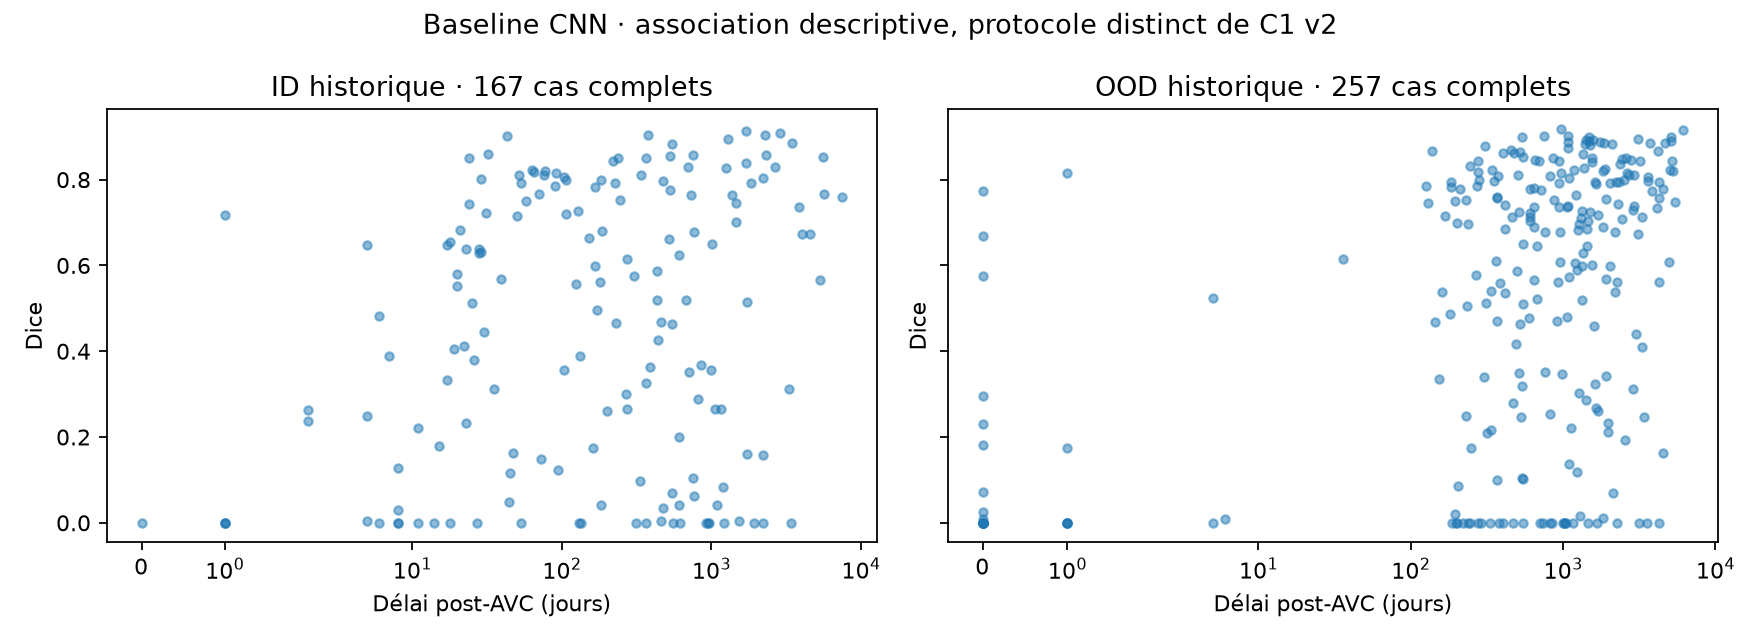
\includegraphics[width=\linewidth]{analysis/reports/s8_historical/time_dice.png}
  \caption{Dice de la baseline CNN historique selon le délai post-AVC, cas complets ID (167) et OOD (257) ; protocole distinct de C1 v2.}
  \label{fig:yosra-s8}
\end{figure}

Ces deux tests sont exploratoires, sans correction de multiplicité.
L'ID a participé au choix historique du modèle et n'est pas un test indépendant.
La partition et le prétraitement diffèrent de C1 v2.
Les résultats des autres baselines sont résumés séparément sur leurs effectifs disponibles, sans comparaison appariée implicite.

Livrables reproductibles : \nolinkurl{analysis/historical_baselines.py}, \nolinkurl{analysis/reports/s8_historical/summary.json}, \nolinkurl{README.md}, \nolinkurl{model_summary.csv}, \nolinkurl{missing_by_center.csv} et \nolinkurl{time_dice.png}.
Les empreintes des fichiers sources sont conservées.

\section{S6 : complément sur l'incertitude}
\label{sec:yosra-s6-incertitude}

Une évaluation complémentaire utilise 912 sujets d'entraînement et 228 sujets réservés, stratifiés parmi les mêmes 25 centres.
Deux classifieurs fixés, régression logistique et forêt aléatoire, sont évalués sur les mêmes sujets.
Les sujets réservés sont ensuite rééchantillonnés 10\,000 fois à l'intérieur de chaque centre, avec les mêmes indices pour toutes les représentations ; l'exactitude équilibrée donne le même poids aux centres.

Pour la forêt aléatoire, le score avant traitement (32 classes) est de 70,1~\%, avec un intervalle percentile conditionnel à 95~\% de [64,6 ; 75,5]~\%.
Après traitement (30 classes), il est de 51,1~\% [45,3 ; 57,0]~\%.
La différence appariée après moins avant est de $-19{,}0$ points [$-25{,}5$ ; $-12{,}6$].
Pour la régression logistique, elle est de $-21{,}5$ points [$-27{,}4$ ; $-15{,}5$] (\nolinkurl{analysis/reports/s6_uncertainty/intervals.csv}, \nolinkurl{analysis/reports/s6_uncertainty/paired_differences.csv}).
La variante après traitement à 150 classes est aussi rapportée pour montrer la sensibilité à la représentation, sans sélectionner uniquement le meilleur score.
La figure~\ref{fig:yosra-s6-incertitude} présente ces intervalles.

\begin{figure}[htbp]
  \centering
  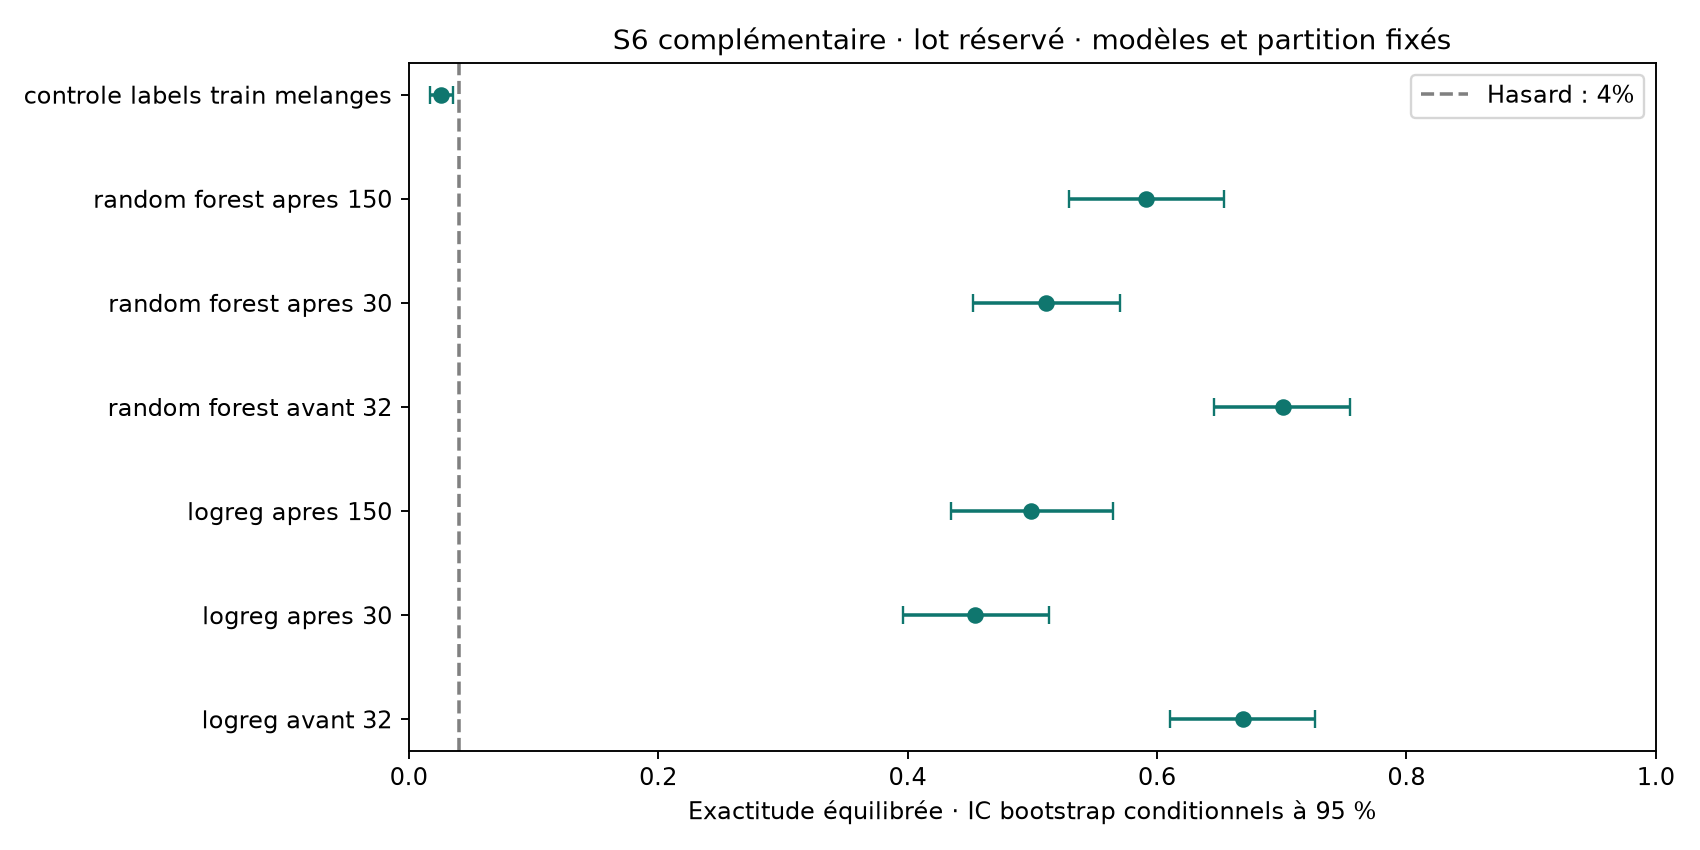
\includegraphics[width=\linewidth]{analysis/reports/s6_uncertainty/confidence_intervals.png}
  \caption{Exactitude équilibrée de la reconnaissance du centre sur le lot réservé, avec IC bootstrap conditionnels à 95~\% (modèles et partition fixés).}
  \label{fig:yosra-s6-incertitude}
\end{figure}

Ces intervalles conditionnent sur les modèles et la partition fixés : ils n'incluent pas la variabilité d'un nouvel entraînement.
La cohorte avait déjà été explorée en S6, et la granularité avant/après reste différente.
Il s'agit d'un complément exploratoire, pas d'une validation externe ni d'un effet causal isolé du prétraitement.
Les centres sont présents dans le train et le test : l'expérience mesure leur reconnaissance, pas la segmentation dans un centre inconnu.
Les moyennes des cinq plis précédentes restent inchangées et ne doivent pas être confondues avec ces nouveaux scores.

Livrables : \nolinkurl{analysis/reports/s6_uncertainty/README.md}, \nolinkurl{intervals.csv}, \nolinkurl{paired_differences.csv}, \nolinkurl{summary.json} et \nolinkurl{confidence_intervals.png}.
Les prédictions individuelles restent dans \nolinkurl{data/analysis/s6_uncertainty/} (hors du dépôt).

\section{Synthèse du contrôle qualité par centre}
\label{sec:yosra-qc}

La synthèse couvre les 1\,453 sujets inventoriés dans 55 centres.
Elle retrouve 1\,415 sujets retenus dans 54 centres, 38 exclus et aucune erreur active.
Les exclusions correspondent aux 37 cas R032 pour espacement non fiable et au cas R065 mis en quarantaine pour annotation hors du support et du recadrage.
Cette synthèse n'ajoute aucune exclusion et ne remplace pas la relecture collective des décisions.

Parmi les 1\,415 sujets retenus, cinq masques sont vides et conservés comme cas négatifs ; 1\,410 sont non vides et aucun statut de masque n'est inconnu.
Le délai post-AVC est disponible pour 1\,073 sujets ; 342 délais sont manquants ou invalides (24,2~\%).
Huit centres retenus n'ont aucun délai utilisable.
Le drapeau CHRONICITY est présent pour 296 sujets et non renseigné pour 1\,119 ; cette absence ne permet pas de déduire un stade clinique.
Deux sujets SOOP portent l'avertissement de fichier de métadonnées vide : cet avertissement de fichier ne recouvre pas toutes les valeurs de délai absentes.

Les effectifs d'exclusion utilisent tout l'inventaire ; les pourcentages de métadonnées utilisent seulement les sujets retenus de chaque centre.
Pour R032, sans sujet retenu, les taux sont non définis plutôt que nuls.
Les colonnes inconnues ne sont pas assimilées à des masques non vides.
Le tableau détaillé, la figure, les motifs d'exclusion et les avertissements sont disponibles dans \nolinkurl{analysis/reports/qc_by_center/} (\nolinkurl{summary.json}, \nolinkurl{qc_by_center.csv}, \nolinkurl{exclusion_reasons.csv}, \nolinkurl{metadata_warnings.csv}).
% La figure qc_by_center.png (55 centres sur trois panneaux) n'est pas insérée : à la largeur de la page, son texte
% ferait environ 3 pt. Elle reste disponible dans analysis/reports/qc_by_center/.
\section{Vérification de l'intégration}
\label{sec:yosra-verification}

Après la fusion des contributions de l'équipe dans \texttt{main}, 310 tests réussissent :
50 pour le pipeline et les analyses, 7 pour l'interface web, 224 pour la généralisation et
l'adaptation (dont des patchs C1 réels) et 29 pour la calibration. Quatorze tests
d'entraînement (\texttt{adaptation/tests/test\_train.py}, \texttt{test\_continual.py}) échouent
sur le Mac de vérification : \texttt{torch.amp.GradScaler} n'existe pas dans torch 2.2.2,
dernière version disponible pour macOS Intel. L'entraînement est exécuté sur Kaggle ;
l'inférence du checkpoint C8 est vérifiée localement
(\texttt{integration/reports/verification.json}).

\setlength{\emergencystretch}{0pt}
. Version LaTeX de docs/pipeline/RAPPORT.md (commit 4540d85) :
% plan, contenu et formulations conservés ; chemins des fichiers sources ajoutés pour chaque chiffre.
% Paquets attendus dans le préambule : babel (french), graphicx, booktabs, makecell, hyperref, float.
% Réglages à mettre dans le préambule du rapport final :
%   \addto\captionsfrench{\def\tablename{Tableau}}   % « Tableau » au lieu de « Table »
%   \hypersetup{hidelinks}                             % liens sans cadre rouge
% Les chemins des figures sont relatifs à la racine du dépôt.
% Statut d'origine (RAPPORT.md) : brouillon scientifique fondé sur les résultats locaux disponibles ; les valeurs
% finales doivent être prises dans les JSON/CSV générés après le dernier QC ; les expériences sans prédictions ou
% checkpoints ne sont pas présentées comme réalisées.

% Chemins de fichiers longs : coupures de ligne aussi permises après « _ » et « - » dans \nolinkurl et \url.
\makeatletter
\g@addto@macro\UrlBreaks{\do\_\do\-}
\makeatother
% Étirement d'urgence limité à ce chapitre (lignes chargées de chemins), remis à zéro à la fin.
\setlength{\emergencystretch}{3em}

\chapter{Données, décalage de domaine et démonstration}
\label{chap:yosra}

\section{Introduction et questions de recherche}
\label{sec:yosra-introduction}

Ce projet étudie la segmentation des lésions d'AVC sur des IRM T1 acquises dans plusieurs centres.
Les différences de scanner, protocole et résolution peuvent modifier la distribution des images.
Notre objectif est de mesurer ce décalage, d'évaluer la généralisation des modèles sur des centres absents de l'entraînement, puis d'étudier la possibilité d'anticiper et de réduire leur perte de performance.

Trois questions structurent le projet : quel est l'écart entre test ID et test OOD ?
Les architectures Transformer améliorent-elles la généralisation par rapport à nnU-Net ?
Quelles techniques de généralisation ou d'adaptation réduisent cet écart ?
La contribution de Yosra fournit le pipeline de données, les partitions communes, les mesures du décalage, les analyses explicatives et l'interface de démonstration.
Les comparaisons de segmentation et l'adaptation continue sont produites par Fayfa et Anas.

\section{Données et contrôle qualité}
\label{sec:yosra-donnees}

L'inventaire local contient 1\,453 paires IRM/masque dans 55 centres.
Le centre R032, soit 37 cas, est exclu provisoirement pour espacement incohérent.
Les métadonnées vides sont signalées sans supprimer une paire utilisable.
Les masques vides sont conservés comme cas négatifs.
Le délai post-AVC reste numérique ; \texttt{CHRONICITY}, codé 1/vide, n'est pas interprété comme une catégorie aigu/subaigu/chronique
(\nolinkurl{analysis/reports/qc_by_center/summary.json}, \nolinkurl{analysis/reports/qc_by_center/exclusion_reasons.csv}).

La livraison v2 contient 1\,415 volumes prétraités, relus et exportés.
Elle exclut les 37 cas R032 et met un cas supplémentaire en quarantaine technique.
Le split v1 est archivé ; v2 retire uniquement ce cas, sans déplacer les autres sujets ni les centres.
La relecture collective de cette quarantaine reste nécessaire ; les annotations brutes sont intactes
(\nolinkurl{preprocessing/reports/release_v2.json}, \nolinkurl{preprocessing/qc_exclusions.json}).

\section{Pipeline Spark}
\label{sec:yosra-pipeline}

Chaque sujet constitue une unité de travail.
Le pipeline réoriente les images en RAS, rééchantillonne à 1~mm isotrope (linéaire pour l'image, plus proche voisin pour les masques), normalise les intensités dans le support cérébral et recadre avec une marge de cinq voxels.
Le support est défini par les intensités supérieures à la valeur de fond estimée ; cette précaution traite notamment le centre R029 dont le fond n'est pas nul.
Cette heuristique reste une limite et doit être examinée sur les cas atypiques.

Le z-score est stocké en \texttt{int16} avec un pas de 0,001.
L'erreur d'arrondi est au plus 0,0005 unité de z-score.
Le validateur utilise cette borne, avec une petite marge numérique, pour la moyenne et l'écart-type ; le fond doit rester exactement nul.
Une signature des entrées et paramètres permet la reprise et chaque paire est accompagnée d'un QC (\nolinkurl{preprocessing/week4.py}).

La boîte de recadrage est déterminée par l'image seule.
Le code existant tolère la suppression de labels hors boîte jusqu'à 1~\% du volume lésionnel.
Ce choix n'est pas une correction clinique des annotations : il doit être documenté et validé.
Le dernier cas dépasse cette tolérance (1,76~\% : 77 voxels sur 4\,376, \nolinkurl{preprocessing/qc_exclusions.json}) et est mis en quarantaine dans v2.
L'option N4 a été ajoutée pour une expérience distincte ; elle n'a pas été appliquée au jeu de référence et aucun bénéfice n'en est revendiqué.

\section{Partitions et absence de fuite}
\label{sec:yosra-partitions}

Le fichier commun \nolinkurl{splits.json} version 2 fixe 916 cas d'entraînement/validation, 231 cas ID et 268 cas OOD (\nolinkurl{preprocessing/reports/release_v2.json}).
Six centres OOD sont intégralement retirés : R008, R028, R031, R034, R053 et SOOP.
Les cinq plis séparent les centres d'entraînement et de validation.
Le test ID de chaque pli est limité aux centres présents dans son entraînement.
Le découpage compte 231 sujets ID au total ; pour le pli~0, le test ID n'en garde que 185, car les 46 autres appartiennent aux centres de validation de ce pli, absents de son entraînement (\nolinkurl{splits.json}, \texttt{folds[0].id\_test}).

La sélection des centres OOD varie taille et distance d'intensité.
Comme la distance participe à cette sélection, un écart de distance ID/OOD n'est pas une découverte indépendante.
Les mesures prédictives doivent utiliser la référence d'entraînement du modèle considéré, pas le pool global.
Aucun hyperparamètre d'alerte ne doit être choisi sur le test OOD.

\section{Benchmark}
\label{sec:yosra-benchmark}

Le pilote existant porte sur huit petits volumes et un essai par configuration.
Les temps de calcul sont 56,59~s, 41,46~s, 27,63~s et 42,54~s pour 1, 2, 4 et 8 workers.
L'accélération maximale mesurée est $\times$2,05 avec quatre workers (\nolinkurl{preprocessing/reports/benchmark_summary.csv}, \nolinkurl{preprocessing/reports/benchmark_scope.json}).
La dégradation à huit workers est compatible avec des coûts de concurrence et de ressources ; ce pilote ne permet pas d'en isoler la cause.
Les workers ne constituent pas des cœurs physiques réservés.
Le démarrage Spark n'entre pas dans \texttt{compute\_seconds}.
Les courbes ne sont pas extrapolées au dataset entier.
La figure~\ref{fig:yosra-benchmark} montre l'accélération mesurée.

\begin{figure}[htbp]
  \centering
  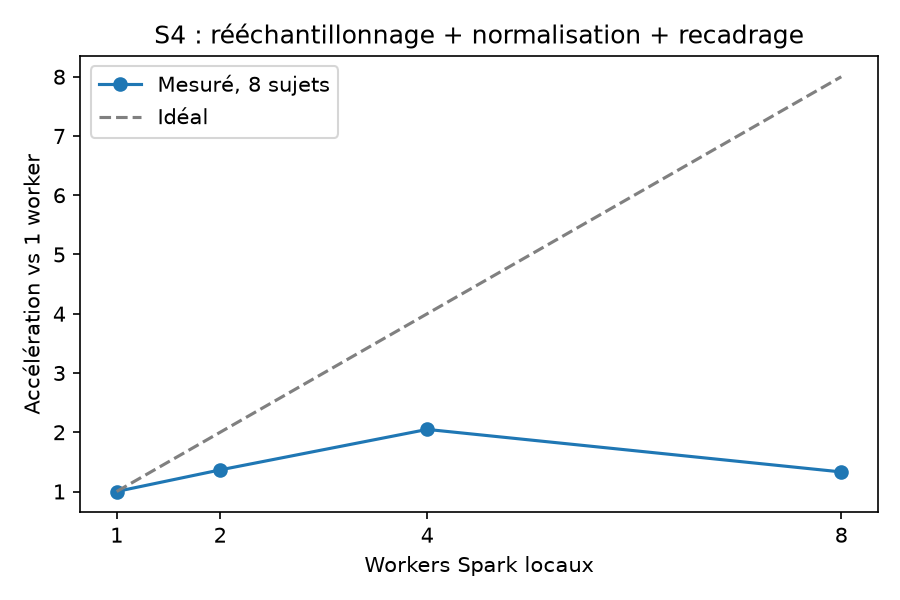
\includegraphics[width=0.6\linewidth]{preprocessing/reports/benchmark_speedup.png}
  \caption{Accélération du prétraitement S4 selon le nombre de workers Spark locaux (8 sujets, un essai).}
  \label{fig:yosra-benchmark}
\end{figure}

\section{Statistiques et empreinte du centre}
\label{sec:yosra-s5-s6}

Les rapports S5 comparent les distributions avant/après prétraitement et mesurent les distances Wasserstein et MMD entre centres et référence.
Le z-score contraint moyenne et variance par scan ; les différences restantes portent donc surtout sur la forme des distributions.
Les échelles avant/après ne sont pas identiques : leur comparaison normalisée reste descriptive.

Le test S6 prédit le centre depuis des histogrammes ou statistiques, avec cinq plis stratifiés, exactitude équilibrée et contrôle à labels mélangés.
Comparer des histogrammes de granularité proche et les mêmes patients permet de mieux isoler l'effet du prétraitement.
Une empreinte reconnaissable n'implique pas à elle seule une baisse du Dice.

Valeurs et figures : \nolinkurl{analysis/reports/post_stats_summary.json}, \nolinkurl{analysis/reports/site_fingerprint_s6.csv}, figures~\ref{fig:yosra-s5-avant-apres}, \ref{fig:yosra-s5-distances} et~\ref{fig:yosra-s6}.
Les versions historiques sur 1\,402 cas ne doivent pas être confondues avec la relance sur 1\,415.
Les versions historiques sur 1\,402 cas sont conservées dans l'historique Git du dépôt
(commit \texttt{5a86471}, fichier \texttt{analysis/reports/post\_stats\_summary.json}).

La relance du 11 novembre couvre 1\,415 sujets dans 54 centres.
La distance relative médiane passe de 0,1315 avant à 0,0376 après, sur la même cohorte disponible.
La corrélation entre Wasserstein et MMD vaut 0,842 pour les centres d'au moins cinq scans.
La médiane de Wasserstein vaut 0,0376 pour ID et 0,0900 pour OOD ; cet écart reste affecté par la sélection initiale des centres (\nolinkurl{analysis/reports/post_stats_summary.json}).
Le test S6 retient 1\,140 scans de 25 centres.
Avec les histogrammes 32 classes avant / 30 classes après et le meilleur des deux classifieurs, l'exactitude équilibrée vaut 69,7~\% puis 48,9~\%.
Le contrôle mélangé vaut 4,0~\%, proche du hasard à 4~\% (\nolinkurl{analysis/reports/site_fingerprint_s6.csv}, \nolinkurl{analysis/reports/site_fingerprint_s6_summary.json}).
Ces chiffres ne mesurent pas la performance de segmentation.

\begin{figure}[p]
  \centering
  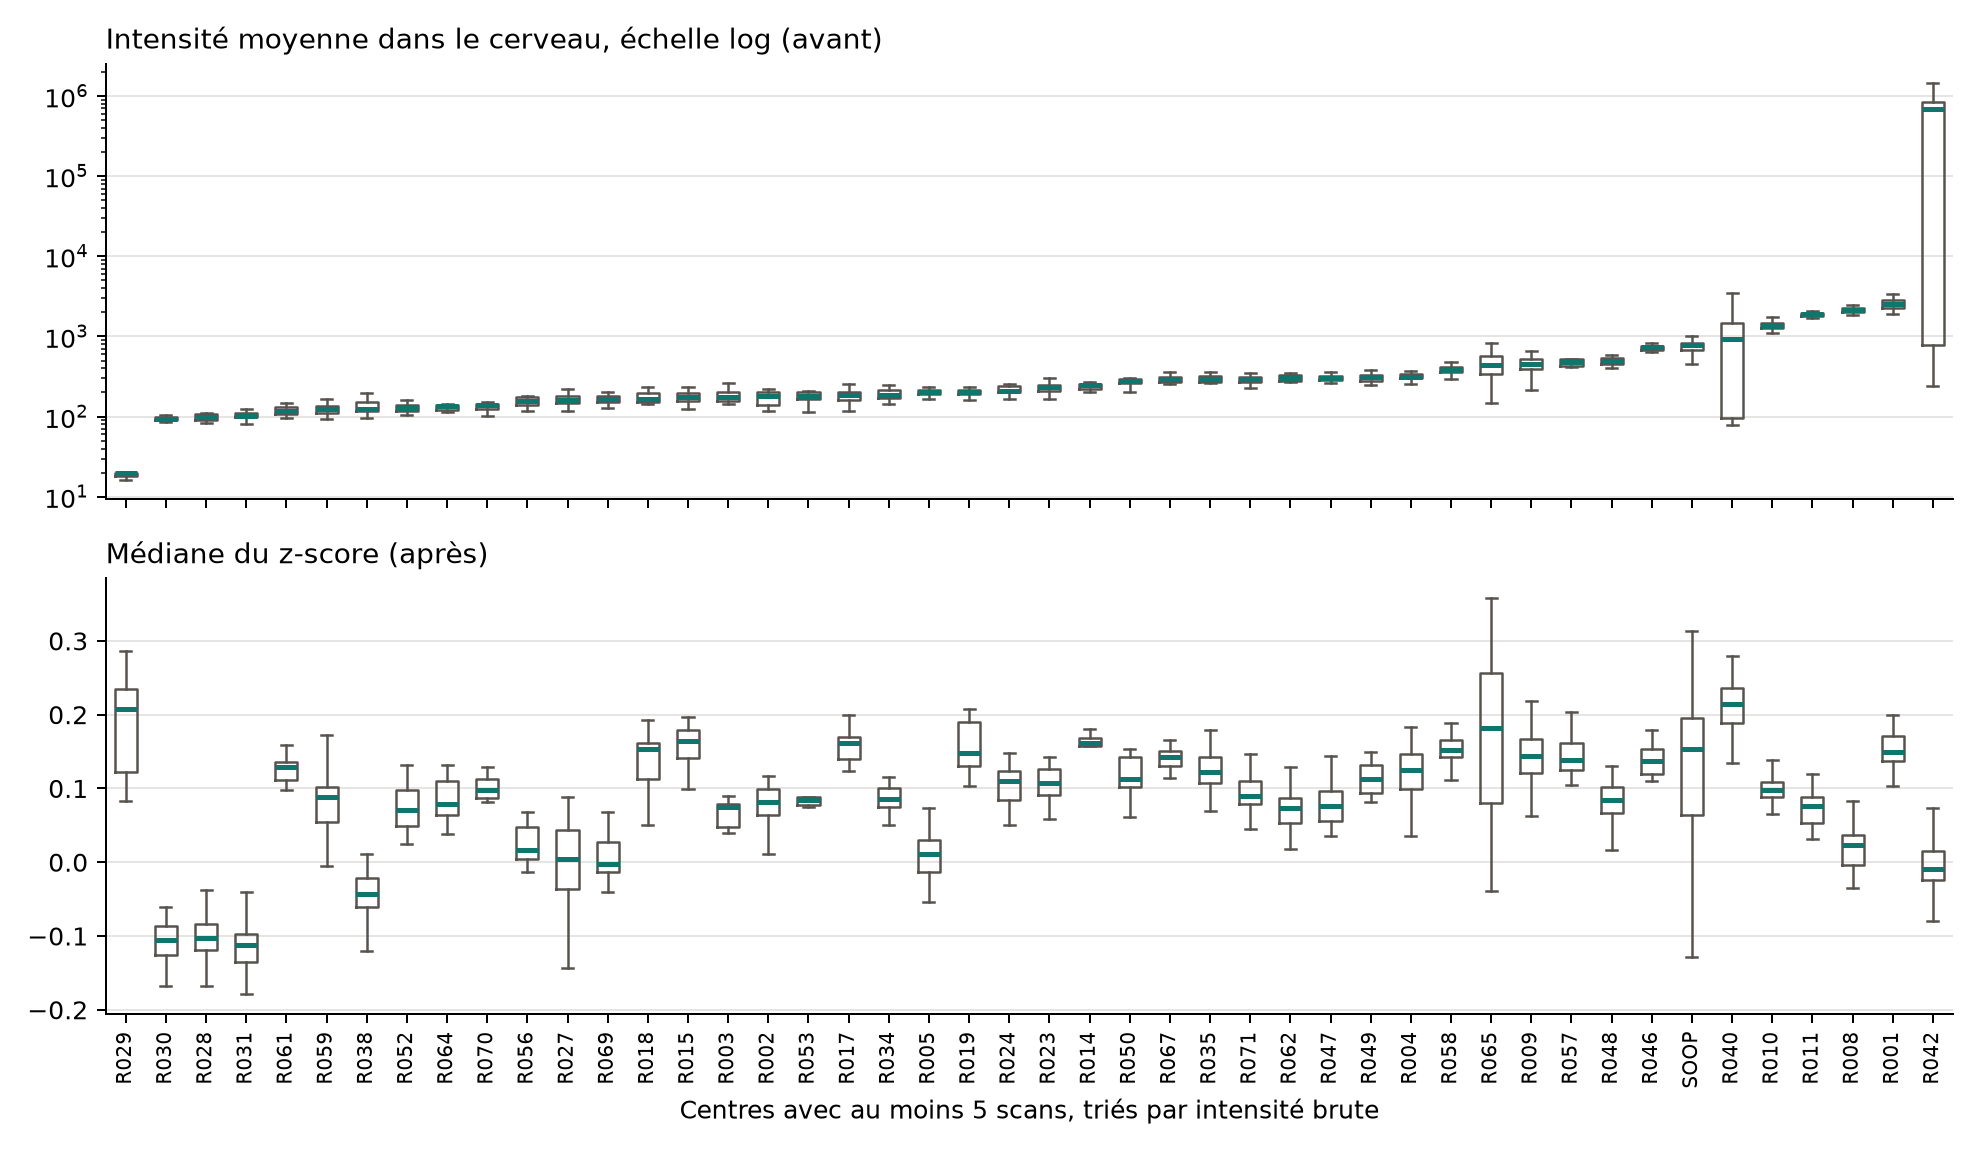
\includegraphics[angle=90,height=0.9\textheight]{figures/s5_avant_apres_par_centre.png}
  \caption{Intensité moyenne dans le cerveau avant prétraitement (échelle log) et médiane du z-score après, par centre (centres d'au moins 5 scans).}
  \label{fig:yosra-s5-avant-apres}
\end{figure}

\begin{figure}[htbp]
  \centering
  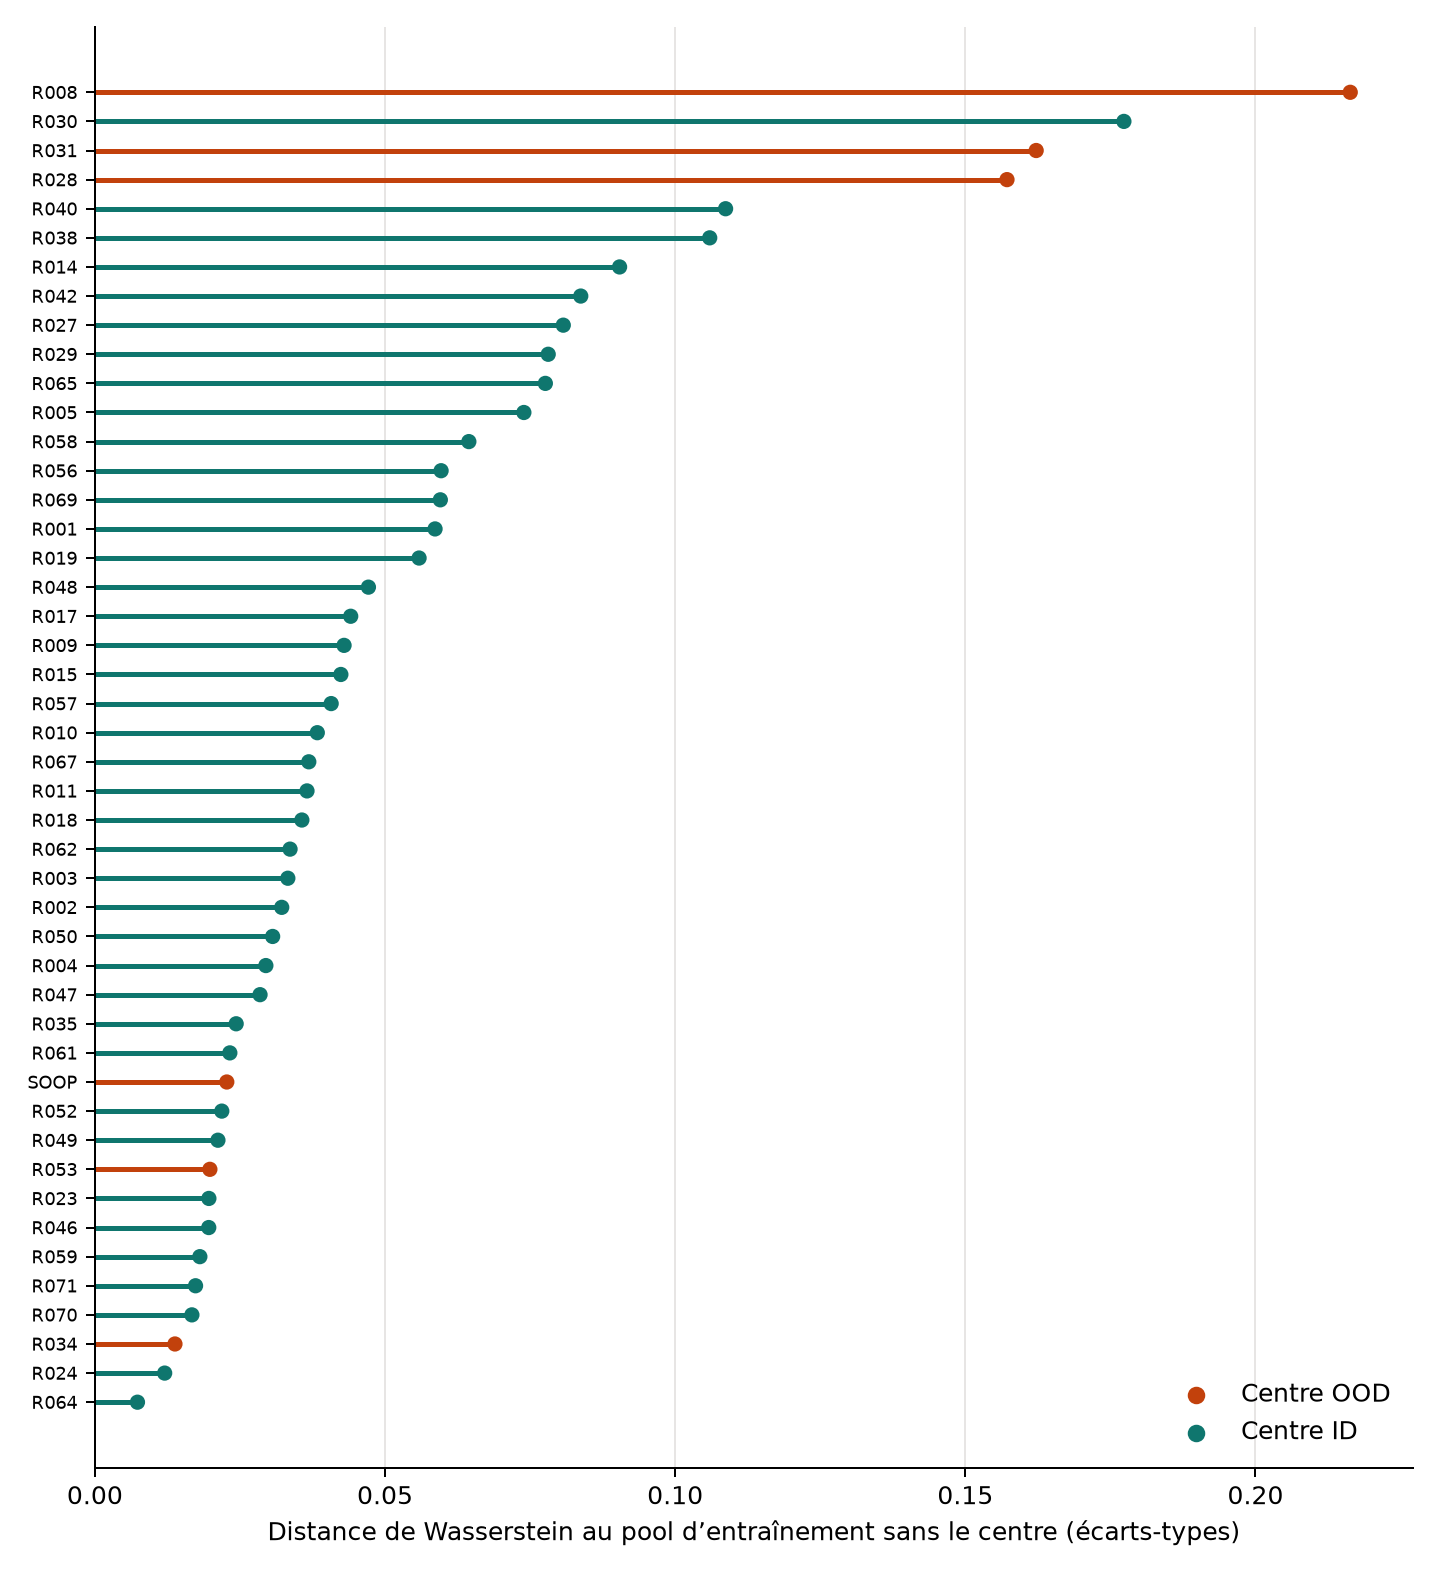
\includegraphics[width=0.85\linewidth]{figures/s5_distances_centres.png}
  \caption{Distance de Wasserstein de chaque centre au pool d'entraînement sans ce centre ; centres OOD en orange.}
  \label{fig:yosra-s5-distances}
\end{figure}

\begin{figure}[htbp]
  \centering
  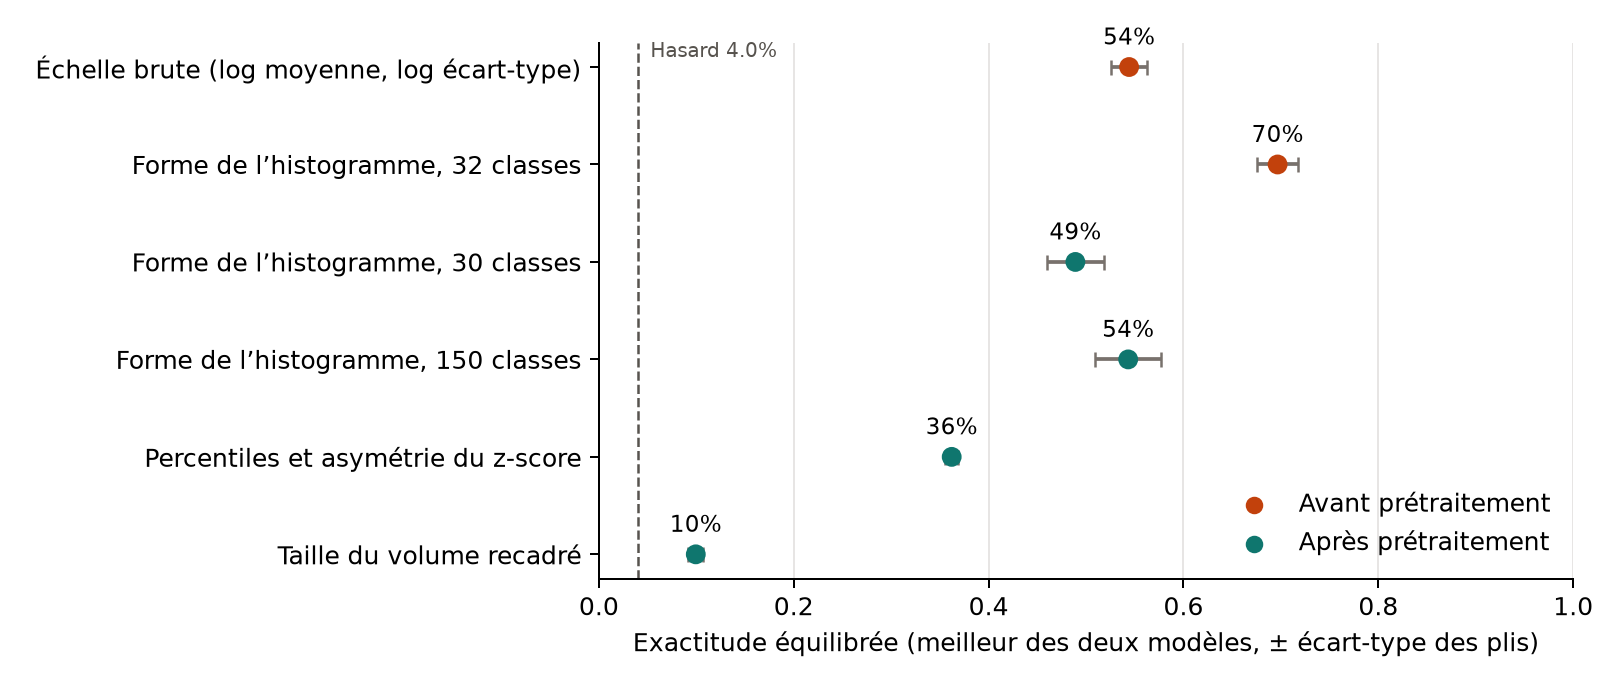
\includegraphics[width=\linewidth]{figures/s6_empreinte_centre.png}
  \caption{Empreinte du centre (S6) : exactitude équilibrée de la prédiction du centre selon la représentation, avant et après prétraitement (hasard : 4~\%).}
  \label{fig:yosra-s6}
\end{figure}

\section{Prédiction d'échec et effet du temps : protocole C1 préparé}
\label{sec:yosra-s7-s8}

S7 met en relation la distance au train du pli et l'erreur $1 - \mathrm{Dice}$ par centre.
Une validation leave-one-center-out produit des prédictions hors calibration.
La régression et le seuil d'alerte sont ajustés uniquement sur les autres centres de validation.
La différence de Dice par rapport au test ID est rapportée séparément.
Sans les résultats C3 de C1, ni corrélation empirique ni performance d'alerte ne peuvent être annoncées.

S8 compare les associations du centre et du délai post-AVC par modèles linéaires emboîtés sur les mêmes cas complets.
Le délai est transformé par $\log(1 + \textrm{jours})$.
Le test de permutation préserve le centre.
Les délais manquants, la sélection des cas et les confusions possibles limitent l'interprétation.
Le protocole n'établit pas une relation causale.

\section{Caractéristiques du réseau (C6 v2)}
\label{sec:yosra-c6}

La version C6 v2 mesure le décalage dans l'espace appris par le réseau plutôt que sur les
intensités. Le modèle C8 (U-Net 3D, augmentation d'intensité, pli 0) est gelé et utilisé en
mode évaluation, sans gradient et sans masque lésionnel. Pour chaque sujet, la sortie du
bottleneck, la couche que lit le classifieur de centre de DANN, est moyennée dans l'espace :
on obtient un vecteur de 320 valeurs par scan.
L'entrée est le volume C1 complet, complété par des zéros jusqu'à un multiple de 16. Le réseau
a été entraîné sur des patchs $96^3$ : sur le volume entier, les normalisations d'instance
portent sur une autre étendue. La même règle est appliquée à tous les scans, ce qui garde la
comparaison entre centres cohérente.

La comparaison d'empreinte baseline / augmentation / DANN demande les checkpoints baseline et
DANN du même protocole ; elle reste à faire.

\section{Démonstration et limites}
\label{sec:yosra-demo}

L'application Gradio affiche les coupes d'une IRM et un masque, calcule le volume lésionnel en mL et accepte une carte d'incertitude.
Un adaptateur permet de brancher le modèle final.
NiiVue fournit une vue 3D locale sur la route \texttt{/viewer/} du même serveur.
ANTsPy peut recaler un template MNI et transférer un atlas de labels ; une inspection visuelle demeure nécessaire avant de nommer les régions.

L'alerte individuelle d'intensité utilise un quantile de validation distinct du seuil par centre.
Elle n'est ni une garantie de performance ni une décision clinique.
En l'absence d'une entrée requise, l'application indique ce qui manque au lieu de créer un résultat.
Le support animé de secours est synthétique et explicitement étiqueté.

\subsection{Interface web du projet}
\label{sec:yosra-frontend}

Une application web (\texttt{frontend/}) présente l'ensemble du projet en dix pages :
vue d'ensemble, avancement du pipeline, contrôle qualité, prétraitement Spark, décalage entre
centres, modèles et Dice, adaptation de domaine, démonstration IRM avec vue 3D, conclusions
et galerie des figures. Le serveur FastAPI lit uniquement les rapports versionnés du dépôt
(\texttt{analysis/reports}, \texttt{preprocessing/reports}, \texttt{baselines/outputs},
\texttt{adaptation/outputs}, \texttt{integration/reports}) : aucun chiffre n'est simulé, et une
expérience absente est signalée comme telle. Chaque page et chaque carte indiquent qui a
produit le résultat. L'interface fonctionne sans étape de construction ni ressource externe ;
seules les figures des dossiers de résultats sont servies, jamais les données IRM. Sept tests
couvrent l'API (\texttt{frontend/tests/test\_server.py}).

\subsection{Branchement du modèle C8}
\label{sec:yosra-c8}

La démonstration (\texttt{demo/app.py}) et l'interface web appellent la fonction désignée par
la variable \texttt{AVC\_PREDICT\_ADAPTER}, au format \texttt{module:fonction}. L'adaptateur de
l'équipe, \texttt{adaptation.demo\_adapter:predict}, applique le prétraitement S4 puis le modèle
retenu (augmentation d'intensité, pli 0) et enregistre le masque en NIfTI \texttt{uint8} dans la
grille de l'IRM reçue. Il demande PyTorch et MONAI, absents de l'environnement de la
démonstration. Le pont \texttt{demo/c8\_bridge.py} lance donc cet adaptateur dans
l'environnement du modèle, dans un processus séparé, et récupère le masque ; la démonstration
utilise \texttt{AVC\_PREDICT\_ADAPTER=c8\_bridge:predict}. Le checkpoint est lu dans
\texttt{data/modeles/unet3d\_intensity\_pli0\_best.pt} (SHA-256 \texttt{ee6b93af\ldots abb6}),
hors du dépôt.

Sur le sujet OOD R034\_sub-r034s003\_ses-1, le rapport de la démonstration donne un volume
lésionnel de 27,058~mL (27\,058 voxels de 1~mm$^3$). Cette valeur concorde avec le volume
prédit lors de l'évaluation du modèle : 27,054~mL dans le fichier \texttt{resultats\_ood\_test.csv}
de la run intensité, conservé hors du dépôt. Sur le sujet OOD R031\_sub-r031s006\_ses-1, envoyé
sans masque à l'interface web, le modèle prédit 33,8~mL pour 27,7~mL annotés, soit un Dice de
0,745, en environ 35~s sur processeur. Ces deux cas vérifient le branchement ; ils ne constituent
pas une évaluation. Le modèle ne produit pas de carte d'incertitude. Cinq tests couvrent les
erreurs du pont (\texttt{tests/test\_c8\_bridge.py}).

\section{Discussion et travaux à terminer}
\label{sec:yosra-discussion}

Les principales limites actuelles sont la quarantaine QC à relire collectivement, le faible nombre de centres pour calibrer un prédicteur d'échec, la dépendance des distances aux effectifs, les métadonnées manquantes et l'absence locale des checkpoints et des Dice correspondant à C1 v2.
Les résultats RQ3 du pli 0 et le checkpoint C8 sont désormais disponibles (chapitre RQ3,
conclusion). Les analyses S7 et S8 sur C1 v2 attendent encore les Dice par sujet, y compris
sur la validation, qui sert à calibrer le seuil d'alerte sans consulter le test. L'empreinte
avant/après DANN attend les checkpoints baseline et DANN. La vidéo de vraie inférence et la
relecture collective restent à faire.
Une analyse S8 historique distincte est disponible plus bas (section~\ref{sec:yosra-s8-historique}).
Les références bibliographiques du document de projet doivent être vérifiées dans leurs publications originales avant d'être reprises dans la version remise.

\section{Compléments vérifiés de la livraison v2}
\label{sec:yosra-livraison}

L'export nnU-Net contient 916 images et labels d'entraînement, 499 images de test (231 ID, 268 OOD) et cinq plis (\nolinkurl{preprocessing/reports/export_v2.json}).
Le contrôle officiel nnU-Net reste à lancer dans l'environnement d'entraînement de Fayfa.
Les autres appartenances de v1 sont conservées.

L'analyse descriptive S8 trouve 1\,073 délais utilisables et 342 manquants ou invalides ; le délai médian est de 365 jours.
Huit centres n'ont aucun délai utilisable.
L'association centre / log-délai (eta carré 0,7475) souligne la nécessité de tenir compte du centre ; elle ne mesure pas l'effet du délai sur le Dice.
Voir \nolinkurl{analysis/reports/s8_metadata/} (\nolinkurl{summary.json}).

Le seuil individuel d'atypie du pli~0 vaut 0,114885 : référence de 733 scans du train, quantile 95~\% sur 183 scans de validation.
Aucun test ID/OOD n'a servi à ce réglage.
Le seuil est enregistré dans \texttt{data/demo/reference\_ood.json} (pli 0, quantile 0,95,
733 scans d'entraînement, 183 de validation), hors du dépôt comme l'ensemble de \texttt{data/}.

Chrome a chargé l'application, produit le rapport synthétique de 2,091~mL, puis affiché les coupes et le rendu 3D NiiVue sans erreur JavaScript (\nolinkurl{docs/pipeline/demo_verification/browser_report.json}).
L'image Docker a été construite et ses routes ainsi que le calcul du rapport ont été testés (\nolinkurl{docs/pipeline/verification.json}).
La vidéo de secours MP4 utilise ces captures réelles d'interface sur un phantom explicitement synthétique ; elle ne montre pas une inférence du réseau.

L'atlas Harvard-Oxford et le template compatible MNI152NLin6Asym ont été récupérés avec leurs sources et empreintes dans \nolinkurl{data/demo/atlas/provenance.json} (hors du dépôt ; copie versionnée : \nolinkurl{docs/pipeline/demo_verification/atlas_provenance.json}).
Les labels corticaux sont prioritaires, puis les labels sous-corticaux décalés de 100 ; les zones non couvertes gardent la valeur zéro.
Le recalage natif exige une relecture anatomique.
Sources : Nilearn Harvard-Oxford\footnote{\url{https://nilearn.github.io/stable/modules/generated/nilearn.datasets.fetch_atlas_harvard_oxford.html}} et TemplateFlow MNI152NLin6Asym\footnote{\url{https://github.com/templateflow/tpl-MNI152NLin6Asym}}.

Le recalage SyN sur l'exemple réel a été exécuté.
Atlas et IRM ont la même grille, les labels restent entiers et 97,75~\% des voxels atlas non nuls se trouvent dans le support d'intensité de l'image (\nolinkurl{docs/pipeline/verification.json}).
La planche locale \nolinkurl{data/demo/registration/qc_overlay.png} (hors du dépôt) a été examinée dans trois plans ; cela ne remplace pas une relecture anatomique experte.
Le rapport régional utilise le masque de référence fourni, sans inférence de réseau.

\section{S8 : résultat exploratoire sur les baselines récupérées}
\label{sec:yosra-s8-historique}

Le 12 novembre, les scores historiques de \texttt{cnn\_pretrained\_freeze-none} ont été rattachés à leur propre partition (903 train, 226 ID validation, 287 OOD), sans les reclasser dans C1 v2.
L'analyse utilise 167 cas ID complets de 31 centres et 257 cas OOD de 12 centres.
En ID, 58 délais manquent ou sont invalides et un Dice est absent ; en OOD, 30 délais manquent ou sont invalides.
Le Dice absent du cas à masque vide n'est pas remplacé par un score supposé.

Après ajustement sur le centre, l'ajout de $\log(1 + \textrm{délai})$ augmente le R$^2$ de 0,000046 en ID ($p$ exploratoire $= 0{,}911$) et de 0,03808 en OOD ($p = 0{,}001$ ; 999 permutations intra-centre pour chaque groupe).
Après ajout de $\log(1 + \textrm{volume lésionnel})$, ces gains sont respectivement 0,000711 et 0,000217 (\nolinkurl{analysis/reports/s8_historical/summary.json}).
L'association OOD dépend donc fortement des variables prises en compte ; elle ne permet pas d'attribuer un effet causal au temps.
Le volume est une analyse de sensibilité, pas un ajustement causal validé.
La figure~\ref{fig:yosra-s8} montre les cas utilisés.

\begin{figure}[htbp]
  \centering
  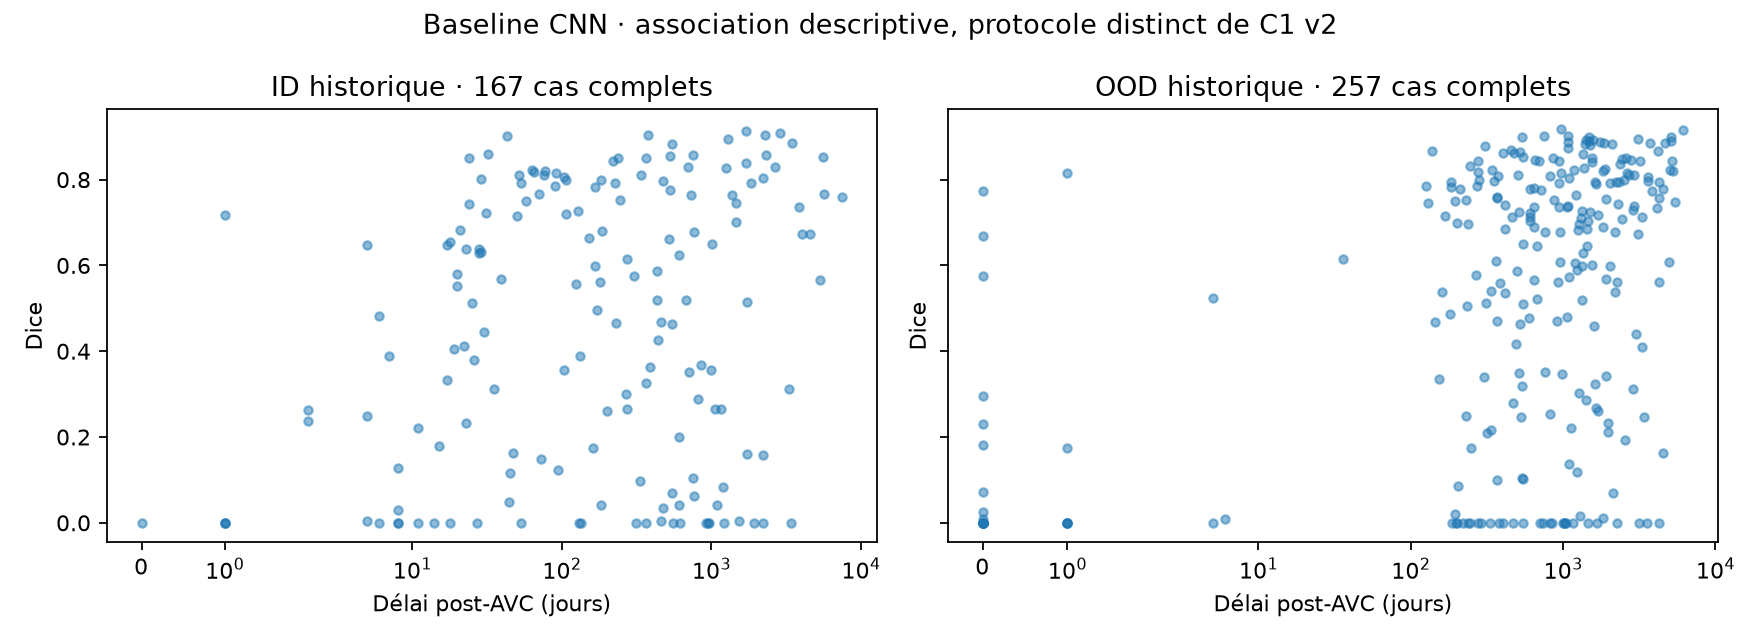
\includegraphics[width=\linewidth]{analysis/reports/s8_historical/time_dice.png}
  \caption{Dice de la baseline CNN historique selon le délai post-AVC, cas complets ID (167) et OOD (257) ; protocole distinct de C1 v2.}
  \label{fig:yosra-s8}
\end{figure}

Ces deux tests sont exploratoires, sans correction de multiplicité.
L'ID a participé au choix historique du modèle et n'est pas un test indépendant.
La partition et le prétraitement diffèrent de C1 v2.
Les résultats des autres baselines sont résumés séparément sur leurs effectifs disponibles, sans comparaison appariée implicite.

Livrables reproductibles : \nolinkurl{analysis/historical_baselines.py}, \nolinkurl{analysis/reports/s8_historical/summary.json}, \nolinkurl{README.md}, \nolinkurl{model_summary.csv}, \nolinkurl{missing_by_center.csv} et \nolinkurl{time_dice.png}.
Les empreintes des fichiers sources sont conservées.

\section{S6 : complément sur l'incertitude}
\label{sec:yosra-s6-incertitude}

Une évaluation complémentaire utilise 912 sujets d'entraînement et 228 sujets réservés, stratifiés parmi les mêmes 25 centres.
Deux classifieurs fixés, régression logistique et forêt aléatoire, sont évalués sur les mêmes sujets.
Les sujets réservés sont ensuite rééchantillonnés 10\,000 fois à l'intérieur de chaque centre, avec les mêmes indices pour toutes les représentations ; l'exactitude équilibrée donne le même poids aux centres.

Pour la forêt aléatoire, le score avant traitement (32 classes) est de 70,1~\%, avec un intervalle percentile conditionnel à 95~\% de [64,6 ; 75,5]~\%.
Après traitement (30 classes), il est de 51,1~\% [45,3 ; 57,0]~\%.
La différence appariée après moins avant est de $-19{,}0$ points [$-25{,}5$ ; $-12{,}6$].
Pour la régression logistique, elle est de $-21{,}5$ points [$-27{,}4$ ; $-15{,}5$] (\nolinkurl{analysis/reports/s6_uncertainty/intervals.csv}, \nolinkurl{analysis/reports/s6_uncertainty/paired_differences.csv}).
La variante après traitement à 150 classes est aussi rapportée pour montrer la sensibilité à la représentation, sans sélectionner uniquement le meilleur score.
La figure~\ref{fig:yosra-s6-incertitude} présente ces intervalles.

\begin{figure}[htbp]
  \centering
  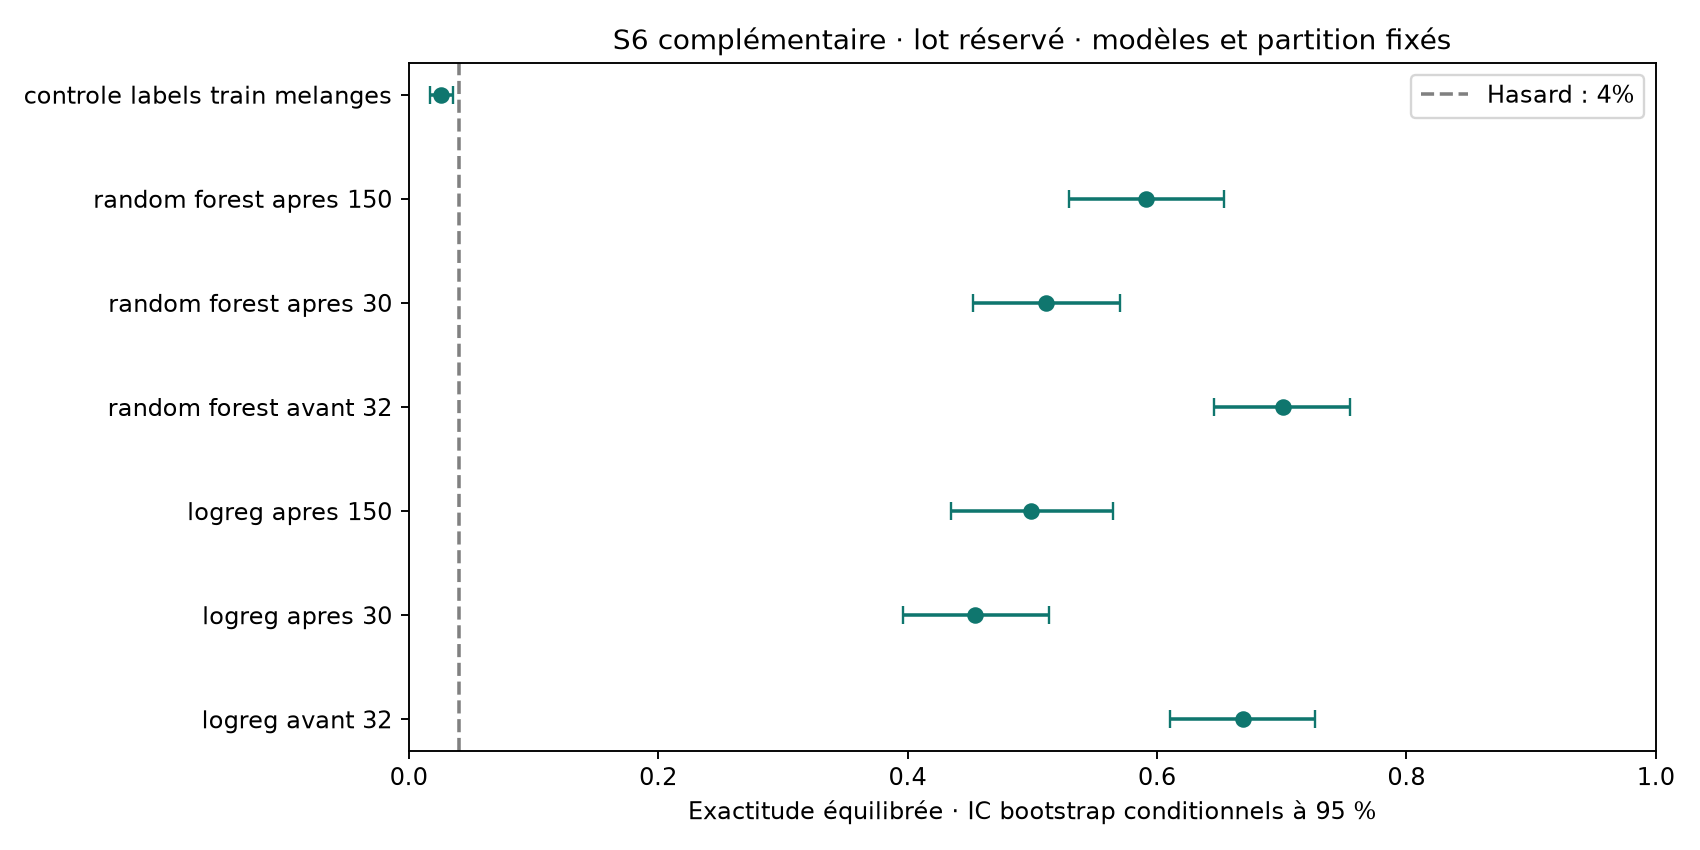
\includegraphics[width=\linewidth]{analysis/reports/s6_uncertainty/confidence_intervals.png}
  \caption{Exactitude équilibrée de la reconnaissance du centre sur le lot réservé, avec IC bootstrap conditionnels à 95~\% (modèles et partition fixés).}
  \label{fig:yosra-s6-incertitude}
\end{figure}

Ces intervalles conditionnent sur les modèles et la partition fixés : ils n'incluent pas la variabilité d'un nouvel entraînement.
La cohorte avait déjà été explorée en S6, et la granularité avant/après reste différente.
Il s'agit d'un complément exploratoire, pas d'une validation externe ni d'un effet causal isolé du prétraitement.
Les centres sont présents dans le train et le test : l'expérience mesure leur reconnaissance, pas la segmentation dans un centre inconnu.
Les moyennes des cinq plis précédentes restent inchangées et ne doivent pas être confondues avec ces nouveaux scores.

Livrables : \nolinkurl{analysis/reports/s6_uncertainty/README.md}, \nolinkurl{intervals.csv}, \nolinkurl{paired_differences.csv}, \nolinkurl{summary.json} et \nolinkurl{confidence_intervals.png}.
Les prédictions individuelles restent dans \nolinkurl{data/analysis/s6_uncertainty/} (hors du dépôt).

\section{Synthèse du contrôle qualité par centre}
\label{sec:yosra-qc}

La synthèse couvre les 1\,453 sujets inventoriés dans 55 centres.
Elle retrouve 1\,415 sujets retenus dans 54 centres, 38 exclus et aucune erreur active.
Les exclusions correspondent aux 37 cas R032 pour espacement non fiable et au cas R065 mis en quarantaine pour annotation hors du support et du recadrage.
Cette synthèse n'ajoute aucune exclusion et ne remplace pas la relecture collective des décisions.

Parmi les 1\,415 sujets retenus, cinq masques sont vides et conservés comme cas négatifs ; 1\,410 sont non vides et aucun statut de masque n'est inconnu.
Le délai post-AVC est disponible pour 1\,073 sujets ; 342 délais sont manquants ou invalides (24,2~\%).
Huit centres retenus n'ont aucun délai utilisable.
Le drapeau CHRONICITY est présent pour 296 sujets et non renseigné pour 1\,119 ; cette absence ne permet pas de déduire un stade clinique.
Deux sujets SOOP portent l'avertissement de fichier de métadonnées vide : cet avertissement de fichier ne recouvre pas toutes les valeurs de délai absentes.

Les effectifs d'exclusion utilisent tout l'inventaire ; les pourcentages de métadonnées utilisent seulement les sujets retenus de chaque centre.
Pour R032, sans sujet retenu, les taux sont non définis plutôt que nuls.
Les colonnes inconnues ne sont pas assimilées à des masques non vides.
Le tableau détaillé, la figure, les motifs d'exclusion et les avertissements sont disponibles dans \nolinkurl{analysis/reports/qc_by_center/} (\nolinkurl{summary.json}, \nolinkurl{qc_by_center.csv}, \nolinkurl{exclusion_reasons.csv}, \nolinkurl{metadata_warnings.csv}).
% La figure qc_by_center.png (55 centres sur trois panneaux) n'est pas insérée : à la largeur de la page, son texte
% ferait environ 3 pt. Elle reste disponible dans analysis/reports/qc_by_center/.
\section{Vérification de l'intégration}
\label{sec:yosra-verification}

Après la fusion des contributions de l'équipe dans \texttt{main}, 310 tests réussissent :
50 pour le pipeline et les analyses, 7 pour l'interface web, 224 pour la généralisation et
l'adaptation (dont des patchs C1 réels) et 29 pour la calibration. Quatorze tests
d'entraînement (\texttt{adaptation/tests/test\_train.py}, \texttt{test\_continual.py}) échouent
sur le Mac de vérification : \texttt{torch.amp.GradScaler} n'existe pas dans torch 2.2.2,
dernière version disponible pour macOS Intel. L'entraînement est exécuté sur Kaggle ;
l'inférence du checkpoint C8 est vérifiée localement
(\texttt{integration/reports/verification.json}).

\setlength{\emergencystretch}{0pt}
. Version LaTeX de docs/pipeline/RAPPORT.md (commit 4540d85) :
% plan, contenu et formulations conservés ; chemins des fichiers sources ajoutés pour chaque chiffre.
% Paquets attendus dans le préambule : babel (french), graphicx, booktabs, makecell, hyperref, float.
% Réglages à mettre dans le préambule du rapport final :
%   \addto\captionsfrench{\def\tablename{Tableau}}   % « Tableau » au lieu de « Table »
%   \hypersetup{hidelinks}                             % liens sans cadre rouge
% Les chemins des figures sont relatifs à la racine du dépôt.
% Statut d'origine (RAPPORT.md) : brouillon scientifique fondé sur les résultats locaux disponibles ; les valeurs
% finales doivent être prises dans les JSON/CSV générés après le dernier QC ; les expériences sans prédictions ou
% checkpoints ne sont pas présentées comme réalisées.

% Chemins de fichiers longs : coupures de ligne aussi permises après « _ » et « - » dans \nolinkurl et \url.
\makeatletter
\g@addto@macro\UrlBreaks{\do\_\do\-}
\makeatother
% Étirement d'urgence limité à ce chapitre (lignes chargées de chemins), remis à zéro à la fin.
\setlength{\emergencystretch}{3em}

\chapter{Données, décalage de domaine et démonstration}
\label{chap:yosra}

\section{Introduction et questions de recherche}
\label{sec:yosra-introduction}

Ce projet étudie la segmentation des lésions d'AVC sur des IRM T1 acquises dans plusieurs centres.
Les différences de scanner, protocole et résolution peuvent modifier la distribution des images.
Notre objectif est de mesurer ce décalage, d'évaluer la généralisation des modèles sur des centres absents de l'entraînement, puis d'étudier la possibilité d'anticiper et de réduire leur perte de performance.

Trois questions structurent le projet : quel est l'écart entre test ID et test OOD ?
Les architectures Transformer améliorent-elles la généralisation par rapport à nnU-Net ?
Quelles techniques de généralisation ou d'adaptation réduisent cet écart ?
La contribution de Yosra fournit le pipeline de données, les partitions communes, les mesures du décalage, les analyses explicatives et l'interface de démonstration.
Les comparaisons de segmentation et l'adaptation continue sont produites par Fayfa et Anas.

\section{Données et contrôle qualité}
\label{sec:yosra-donnees}

L'inventaire local contient 1\,453 paires IRM/masque dans 55 centres.
Le centre R032, soit 37 cas, est exclu provisoirement pour espacement incohérent.
Les métadonnées vides sont signalées sans supprimer une paire utilisable.
Les masques vides sont conservés comme cas négatifs.
Le délai post-AVC reste numérique ; \texttt{CHRONICITY}, codé 1/vide, n'est pas interprété comme une catégorie aigu/subaigu/chronique
(\nolinkurl{analysis/reports/qc_by_center/summary.json}, \nolinkurl{analysis/reports/qc_by_center/exclusion_reasons.csv}).

La livraison v2 contient 1\,415 volumes prétraités, relus et exportés.
Elle exclut les 37 cas R032 et met un cas supplémentaire en quarantaine technique.
Le split v1 est archivé ; v2 retire uniquement ce cas, sans déplacer les autres sujets ni les centres.
La relecture collective de cette quarantaine reste nécessaire ; les annotations brutes sont intactes
(\nolinkurl{preprocessing/reports/release_v2.json}, \nolinkurl{preprocessing/qc_exclusions.json}).

\section{Pipeline Spark}
\label{sec:yosra-pipeline}

Chaque sujet constitue une unité de travail.
Le pipeline réoriente les images en RAS, rééchantillonne à 1~mm isotrope (linéaire pour l'image, plus proche voisin pour les masques), normalise les intensités dans le support cérébral et recadre avec une marge de cinq voxels.
Le support est défini par les intensités supérieures à la valeur de fond estimée ; cette précaution traite notamment le centre R029 dont le fond n'est pas nul.
Cette heuristique reste une limite et doit être examinée sur les cas atypiques.

Le z-score est stocké en \texttt{int16} avec un pas de 0,001.
L'erreur d'arrondi est au plus 0,0005 unité de z-score.
Le validateur utilise cette borne, avec une petite marge numérique, pour la moyenne et l'écart-type ; le fond doit rester exactement nul.
Une signature des entrées et paramètres permet la reprise et chaque paire est accompagnée d'un QC (\nolinkurl{preprocessing/week4.py}).

La boîte de recadrage est déterminée par l'image seule.
Le code existant tolère la suppression de labels hors boîte jusqu'à 1~\% du volume lésionnel.
Ce choix n'est pas une correction clinique des annotations : il doit être documenté et validé.
Le dernier cas dépasse cette tolérance (1,76~\% : 77 voxels sur 4\,376, \nolinkurl{preprocessing/qc_exclusions.json}) et est mis en quarantaine dans v2.
L'option N4 a été ajoutée pour une expérience distincte ; elle n'a pas été appliquée au jeu de référence et aucun bénéfice n'en est revendiqué.

\section{Partitions et absence de fuite}
\label{sec:yosra-partitions}

Le fichier commun \nolinkurl{splits.json} version 2 fixe 916 cas d'entraînement/validation, 231 cas ID et 268 cas OOD (\nolinkurl{preprocessing/reports/release_v2.json}).
Six centres OOD sont intégralement retirés : R008, R028, R031, R034, R053 et SOOP.
Les cinq plis séparent les centres d'entraînement et de validation.
Le test ID de chaque pli est limité aux centres présents dans son entraînement.
Le découpage compte 231 sujets ID au total ; pour le pli~0, le test ID n'en garde que 185, car les 46 autres appartiennent aux centres de validation de ce pli, absents de son entraînement (\nolinkurl{splits.json}, \texttt{folds[0].id\_test}).

La sélection des centres OOD varie taille et distance d'intensité.
Comme la distance participe à cette sélection, un écart de distance ID/OOD n'est pas une découverte indépendante.
Les mesures prédictives doivent utiliser la référence d'entraînement du modèle considéré, pas le pool global.
Aucun hyperparamètre d'alerte ne doit être choisi sur le test OOD.

\section{Benchmark}
\label{sec:yosra-benchmark}

Le pilote existant porte sur huit petits volumes et un essai par configuration.
Les temps de calcul sont 56,59~s, 41,46~s, 27,63~s et 42,54~s pour 1, 2, 4 et 8 workers.
L'accélération maximale mesurée est $\times$2,05 avec quatre workers (\nolinkurl{preprocessing/reports/benchmark_summary.csv}, \nolinkurl{preprocessing/reports/benchmark_scope.json}).
La dégradation à huit workers est compatible avec des coûts de concurrence et de ressources ; ce pilote ne permet pas d'en isoler la cause.
Les workers ne constituent pas des cœurs physiques réservés.
Le démarrage Spark n'entre pas dans \texttt{compute\_seconds}.
Les courbes ne sont pas extrapolées au dataset entier.
La figure~\ref{fig:yosra-benchmark} montre l'accélération mesurée.

\begin{figure}[htbp]
  \centering
  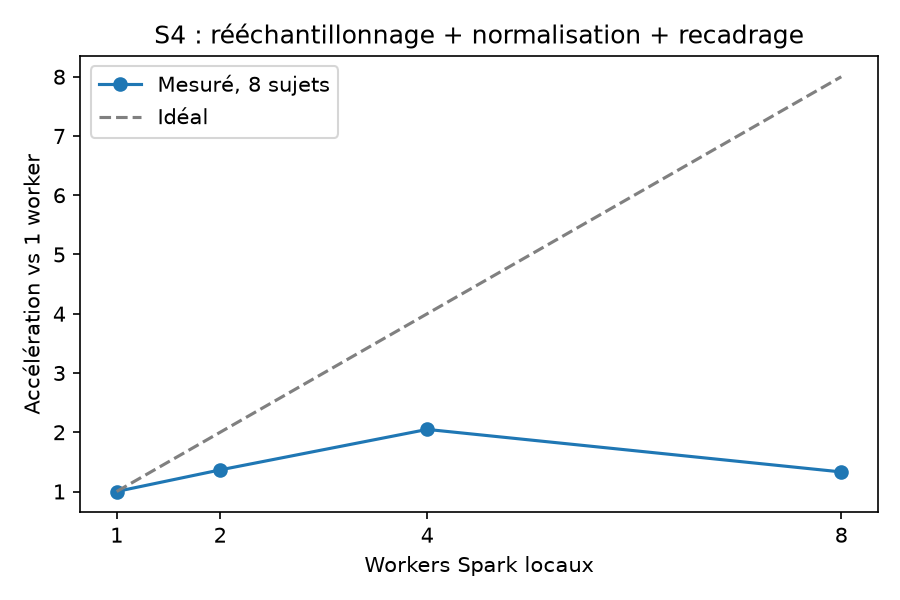
\includegraphics[width=0.6\linewidth]{preprocessing/reports/benchmark_speedup.png}
  \caption{Accélération du prétraitement S4 selon le nombre de workers Spark locaux (8 sujets, un essai).}
  \label{fig:yosra-benchmark}
\end{figure}

\section{Statistiques et empreinte du centre}
\label{sec:yosra-s5-s6}

Les rapports S5 comparent les distributions avant/après prétraitement et mesurent les distances Wasserstein et MMD entre centres et référence.
Le z-score contraint moyenne et variance par scan ; les différences restantes portent donc surtout sur la forme des distributions.
Les échelles avant/après ne sont pas identiques : leur comparaison normalisée reste descriptive.

Le test S6 prédit le centre depuis des histogrammes ou statistiques, avec cinq plis stratifiés, exactitude équilibrée et contrôle à labels mélangés.
Comparer des histogrammes de granularité proche et les mêmes patients permet de mieux isoler l'effet du prétraitement.
Une empreinte reconnaissable n'implique pas à elle seule une baisse du Dice.

Valeurs et figures : \nolinkurl{analysis/reports/post_stats_summary.json}, \nolinkurl{analysis/reports/site_fingerprint_s6.csv}, figures~\ref{fig:yosra-s5-avant-apres}, \ref{fig:yosra-s5-distances} et~\ref{fig:yosra-s6}.
Les versions historiques sur 1\,402 cas ne doivent pas être confondues avec la relance sur 1\,415.
Les versions historiques sur 1\,402 cas sont conservées dans l'historique Git du dépôt
(commit \texttt{5a86471}, fichier \texttt{analysis/reports/post\_stats\_summary.json}).

La relance du 11 novembre couvre 1\,415 sujets dans 54 centres.
La distance relative médiane passe de 0,1315 avant à 0,0376 après, sur la même cohorte disponible.
La corrélation entre Wasserstein et MMD vaut 0,842 pour les centres d'au moins cinq scans.
La médiane de Wasserstein vaut 0,0376 pour ID et 0,0900 pour OOD ; cet écart reste affecté par la sélection initiale des centres (\nolinkurl{analysis/reports/post_stats_summary.json}).
Le test S6 retient 1\,140 scans de 25 centres.
Avec les histogrammes 32 classes avant / 30 classes après et le meilleur des deux classifieurs, l'exactitude équilibrée vaut 69,7~\% puis 48,9~\%.
Le contrôle mélangé vaut 4,0~\%, proche du hasard à 4~\% (\nolinkurl{analysis/reports/site_fingerprint_s6.csv}, \nolinkurl{analysis/reports/site_fingerprint_s6_summary.json}).
Ces chiffres ne mesurent pas la performance de segmentation.

\begin{figure}[p]
  \centering
  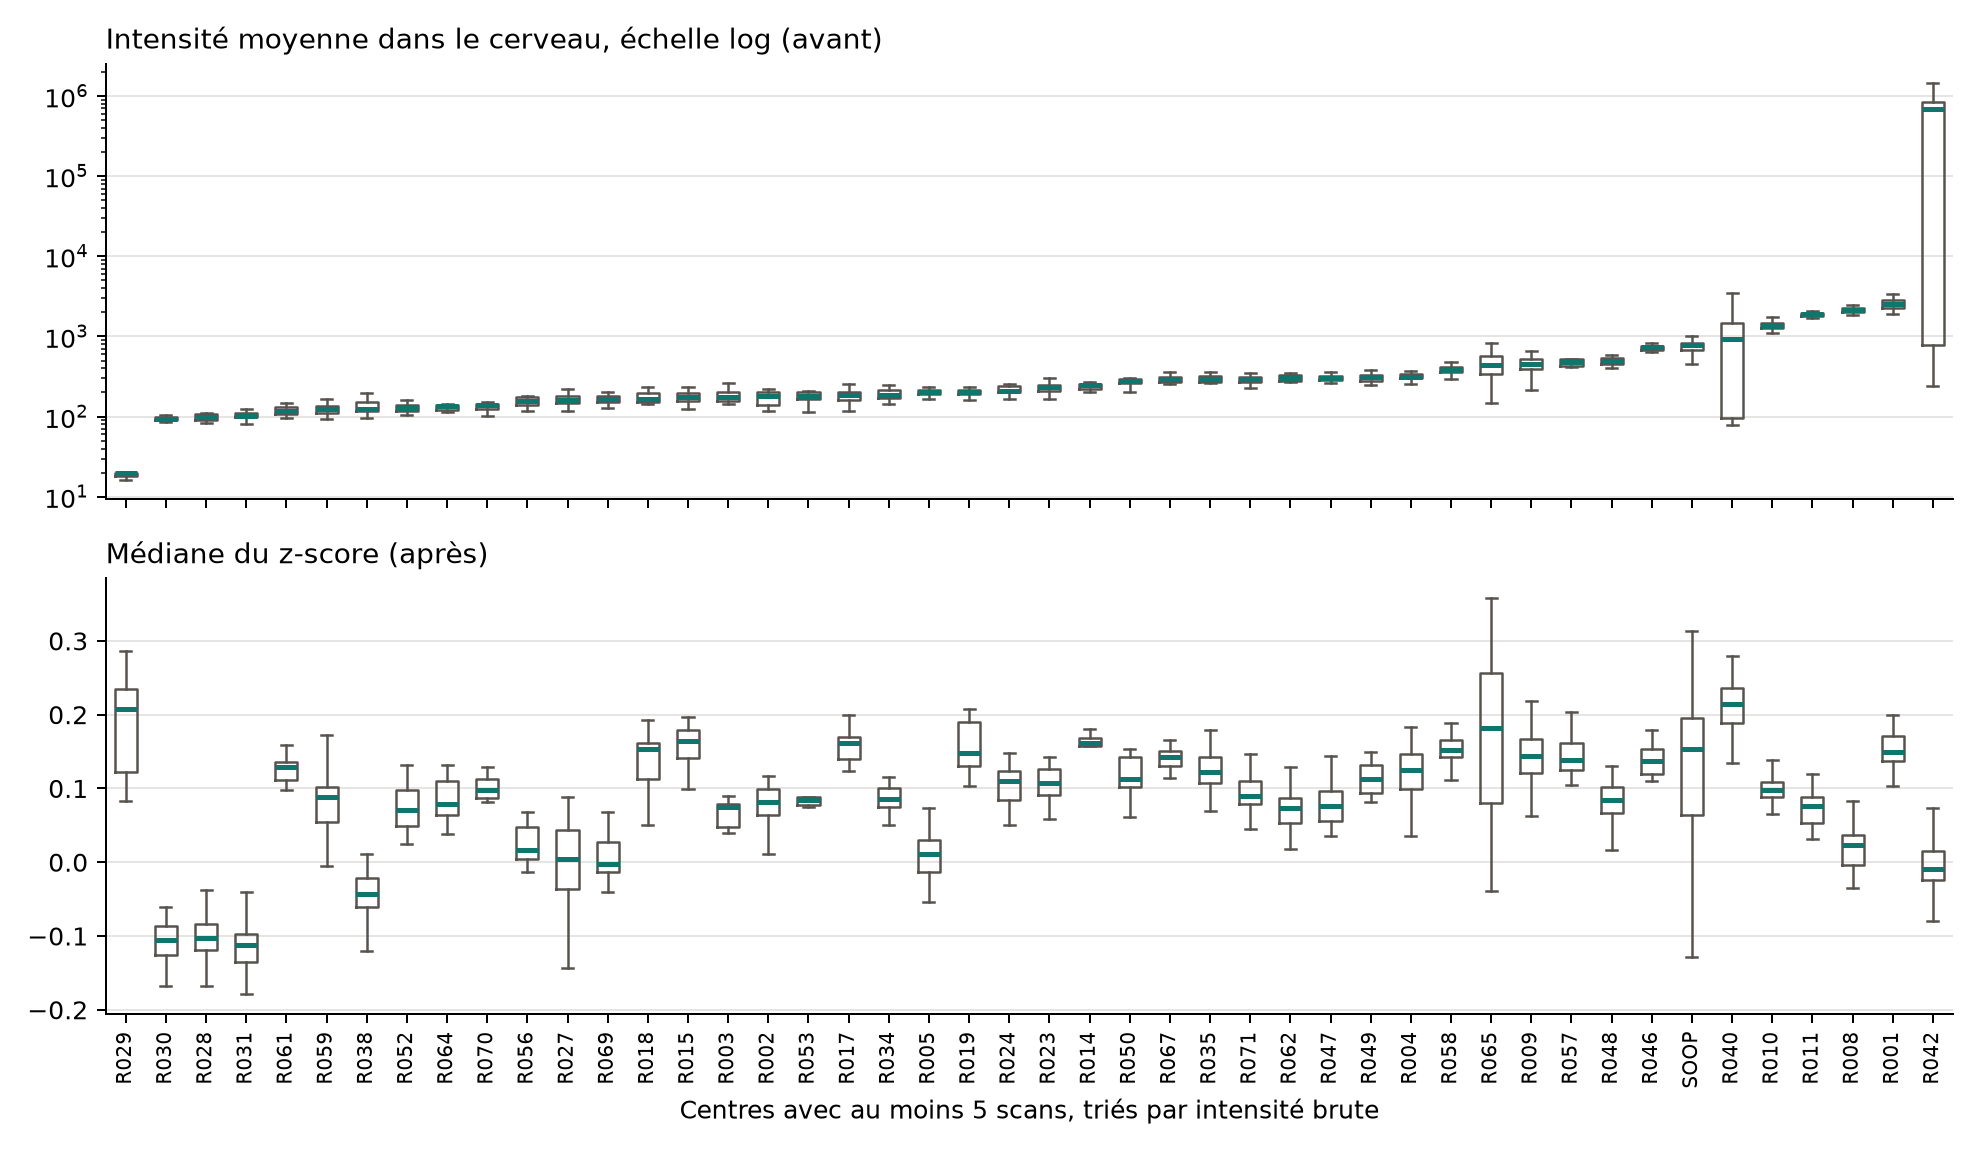
\includegraphics[angle=90,height=0.9\textheight]{figures/s5_avant_apres_par_centre.png}
  \caption{Intensité moyenne dans le cerveau avant prétraitement (échelle log) et médiane du z-score après, par centre (centres d'au moins 5 scans).}
  \label{fig:yosra-s5-avant-apres}
\end{figure}

\begin{figure}[htbp]
  \centering
  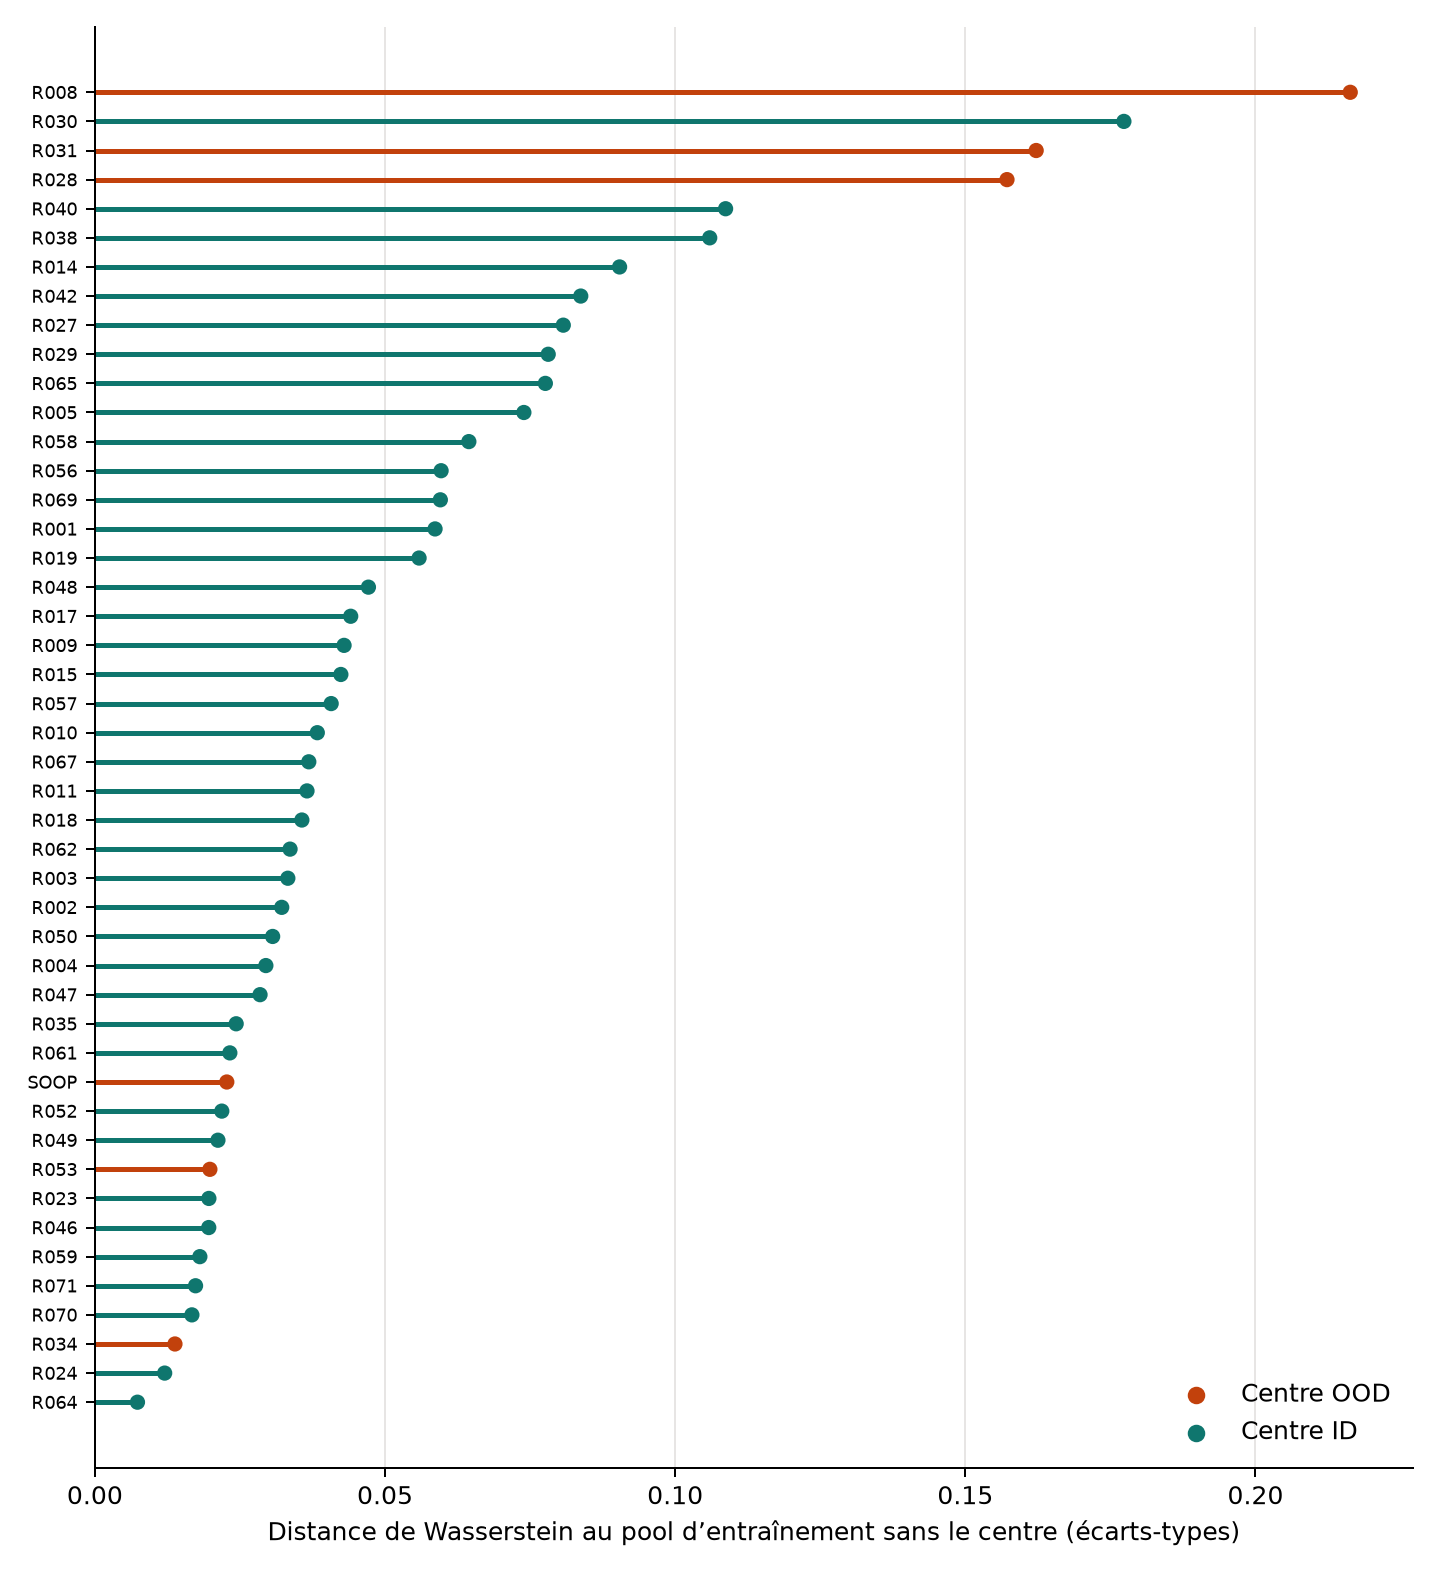
\includegraphics[width=0.85\linewidth]{figures/s5_distances_centres.png}
  \caption{Distance de Wasserstein de chaque centre au pool d'entraînement sans ce centre ; centres OOD en orange.}
  \label{fig:yosra-s5-distances}
\end{figure}

\begin{figure}[htbp]
  \centering
  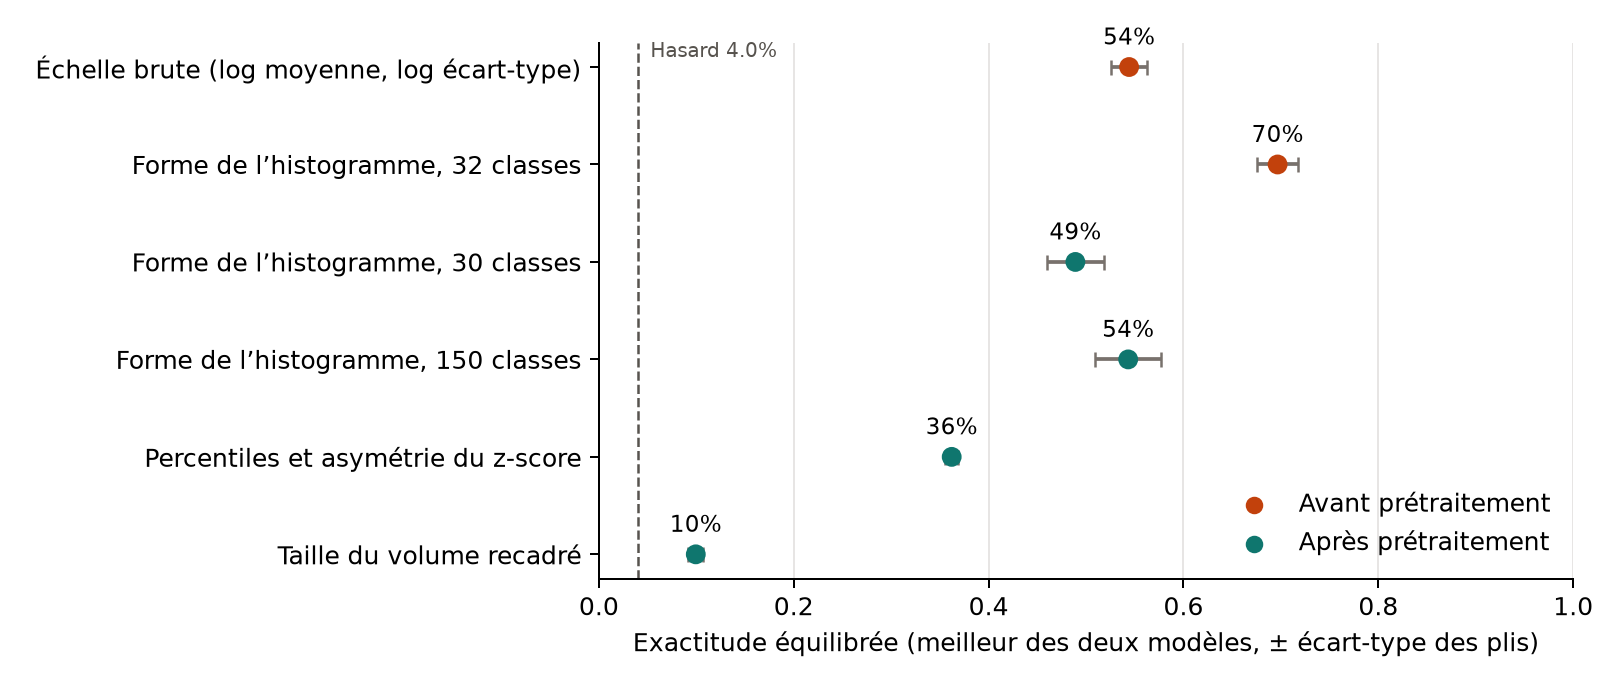
\includegraphics[width=\linewidth]{figures/s6_empreinte_centre.png}
  \caption{Empreinte du centre (S6) : exactitude équilibrée de la prédiction du centre selon la représentation, avant et après prétraitement (hasard : 4~\%).}
  \label{fig:yosra-s6}
\end{figure}

\section{Prédiction d'échec et effet du temps : protocole C1 préparé}
\label{sec:yosra-s7-s8}

S7 met en relation la distance au train du pli et l'erreur $1 - \mathrm{Dice}$ par centre.
Une validation leave-one-center-out produit des prédictions hors calibration.
La régression et le seuil d'alerte sont ajustés uniquement sur les autres centres de validation.
La différence de Dice par rapport au test ID est rapportée séparément.
Sans les résultats C3 de C1, ni corrélation empirique ni performance d'alerte ne peuvent être annoncées.

S8 compare les associations du centre et du délai post-AVC par modèles linéaires emboîtés sur les mêmes cas complets.
Le délai est transformé par $\log(1 + \textrm{jours})$.
Le test de permutation préserve le centre.
Les délais manquants, la sélection des cas et les confusions possibles limitent l'interprétation.
Le protocole n'établit pas une relation causale.

\section{Caractéristiques du réseau (C6 v2)}
\label{sec:yosra-c6}

La version C6 v2 mesure le décalage dans l'espace appris par le réseau plutôt que sur les
intensités. Le modèle C8 (U-Net 3D, augmentation d'intensité, pli 0) est gelé et utilisé en
mode évaluation, sans gradient et sans masque lésionnel. Pour chaque sujet, la sortie du
bottleneck, la couche que lit le classifieur de centre de DANN, est moyennée dans l'espace :
on obtient un vecteur de 320 valeurs par scan.
L'entrée est le volume C1 complet, complété par des zéros jusqu'à un multiple de 16. Le réseau
a été entraîné sur des patchs $96^3$ : sur le volume entier, les normalisations d'instance
portent sur une autre étendue. La même règle est appliquée à tous les scans, ce qui garde la
comparaison entre centres cohérente.

La comparaison d'empreinte baseline / augmentation / DANN demande les checkpoints baseline et
DANN du même protocole ; elle reste à faire.

\section{Démonstration et limites}
\label{sec:yosra-demo}

L'application Gradio affiche les coupes d'une IRM et un masque, calcule le volume lésionnel en mL et accepte une carte d'incertitude.
Un adaptateur permet de brancher le modèle final.
NiiVue fournit une vue 3D locale sur la route \texttt{/viewer/} du même serveur.
ANTsPy peut recaler un template MNI et transférer un atlas de labels ; une inspection visuelle demeure nécessaire avant de nommer les régions.

L'alerte individuelle d'intensité utilise un quantile de validation distinct du seuil par centre.
Elle n'est ni une garantie de performance ni une décision clinique.
En l'absence d'une entrée requise, l'application indique ce qui manque au lieu de créer un résultat.
Le support animé de secours est synthétique et explicitement étiqueté.

\subsection{Interface web du projet}
\label{sec:yosra-frontend}

Une application web (\texttt{frontend/}) présente l'ensemble du projet en dix pages :
vue d'ensemble, avancement du pipeline, contrôle qualité, prétraitement Spark, décalage entre
centres, modèles et Dice, adaptation de domaine, démonstration IRM avec vue 3D, conclusions
et galerie des figures. Le serveur FastAPI lit uniquement les rapports versionnés du dépôt
(\texttt{analysis/reports}, \texttt{preprocessing/reports}, \texttt{baselines/outputs},
\texttt{adaptation/outputs}, \texttt{integration/reports}) : aucun chiffre n'est simulé, et une
expérience absente est signalée comme telle. Chaque page et chaque carte indiquent qui a
produit le résultat. L'interface fonctionne sans étape de construction ni ressource externe ;
seules les figures des dossiers de résultats sont servies, jamais les données IRM. Sept tests
couvrent l'API (\texttt{frontend/tests/test\_server.py}).

\subsection{Branchement du modèle C8}
\label{sec:yosra-c8}

La démonstration (\texttt{demo/app.py}) et l'interface web appellent la fonction désignée par
la variable \texttt{AVC\_PREDICT\_ADAPTER}, au format \texttt{module:fonction}. L'adaptateur de
l'équipe, \texttt{adaptation.demo\_adapter:predict}, applique le prétraitement S4 puis le modèle
retenu (augmentation d'intensité, pli 0) et enregistre le masque en NIfTI \texttt{uint8} dans la
grille de l'IRM reçue. Il demande PyTorch et MONAI, absents de l'environnement de la
démonstration. Le pont \texttt{demo/c8\_bridge.py} lance donc cet adaptateur dans
l'environnement du modèle, dans un processus séparé, et récupère le masque ; la démonstration
utilise \texttt{AVC\_PREDICT\_ADAPTER=c8\_bridge:predict}. Le checkpoint est lu dans
\texttt{data/modeles/unet3d\_intensity\_pli0\_best.pt} (SHA-256 \texttt{ee6b93af\ldots abb6}),
hors du dépôt.

Sur le sujet OOD R034\_sub-r034s003\_ses-1, le rapport de la démonstration donne un volume
lésionnel de 27,058~mL (27\,058 voxels de 1~mm$^3$). Cette valeur concorde avec le volume
prédit lors de l'évaluation du modèle : 27,054~mL dans le fichier \texttt{resultats\_ood\_test.csv}
de la run intensité, conservé hors du dépôt. Sur le sujet OOD R031\_sub-r031s006\_ses-1, envoyé
sans masque à l'interface web, le modèle prédit 33,8~mL pour 27,7~mL annotés, soit un Dice de
0,745, en environ 35~s sur processeur. Ces deux cas vérifient le branchement ; ils ne constituent
pas une évaluation. Le modèle ne produit pas de carte d'incertitude. Cinq tests couvrent les
erreurs du pont (\texttt{tests/test\_c8\_bridge.py}).

\section{Discussion et travaux à terminer}
\label{sec:yosra-discussion}

Les principales limites actuelles sont la quarantaine QC à relire collectivement, le faible nombre de centres pour calibrer un prédicteur d'échec, la dépendance des distances aux effectifs, les métadonnées manquantes et l'absence locale des checkpoints et des Dice correspondant à C1 v2.
Les résultats RQ3 du pli 0 et le checkpoint C8 sont désormais disponibles (chapitre RQ3,
conclusion). Les analyses S7 et S8 sur C1 v2 attendent encore les Dice par sujet, y compris
sur la validation, qui sert à calibrer le seuil d'alerte sans consulter le test. L'empreinte
avant/après DANN attend les checkpoints baseline et DANN. La vidéo de vraie inférence et la
relecture collective restent à faire.
Une analyse S8 historique distincte est disponible plus bas (section~\ref{sec:yosra-s8-historique}).
Les références bibliographiques du document de projet doivent être vérifiées dans leurs publications originales avant d'être reprises dans la version remise.

\section{Compléments vérifiés de la livraison v2}
\label{sec:yosra-livraison}

L'export nnU-Net contient 916 images et labels d'entraînement, 499 images de test (231 ID, 268 OOD) et cinq plis (\nolinkurl{preprocessing/reports/export_v2.json}).
Le contrôle officiel nnU-Net reste à lancer dans l'environnement d'entraînement de Fayfa.
Les autres appartenances de v1 sont conservées.

L'analyse descriptive S8 trouve 1\,073 délais utilisables et 342 manquants ou invalides ; le délai médian est de 365 jours.
Huit centres n'ont aucun délai utilisable.
L'association centre / log-délai (eta carré 0,7475) souligne la nécessité de tenir compte du centre ; elle ne mesure pas l'effet du délai sur le Dice.
Voir \nolinkurl{analysis/reports/s8_metadata/} (\nolinkurl{summary.json}).

Le seuil individuel d'atypie du pli~0 vaut 0,114885 : référence de 733 scans du train, quantile 95~\% sur 183 scans de validation.
Aucun test ID/OOD n'a servi à ce réglage.
Le seuil est enregistré dans \texttt{data/demo/reference\_ood.json} (pli 0, quantile 0,95,
733 scans d'entraînement, 183 de validation), hors du dépôt comme l'ensemble de \texttt{data/}.

Chrome a chargé l'application, produit le rapport synthétique de 2,091~mL, puis affiché les coupes et le rendu 3D NiiVue sans erreur JavaScript (\nolinkurl{docs/pipeline/demo_verification/browser_report.json}).
L'image Docker a été construite et ses routes ainsi que le calcul du rapport ont été testés (\nolinkurl{docs/pipeline/verification.json}).
La vidéo de secours MP4 utilise ces captures réelles d'interface sur un phantom explicitement synthétique ; elle ne montre pas une inférence du réseau.

L'atlas Harvard-Oxford et le template compatible MNI152NLin6Asym ont été récupérés avec leurs sources et empreintes dans \nolinkurl{data/demo/atlas/provenance.json} (hors du dépôt ; copie versionnée : \nolinkurl{docs/pipeline/demo_verification/atlas_provenance.json}).
Les labels corticaux sont prioritaires, puis les labels sous-corticaux décalés de 100 ; les zones non couvertes gardent la valeur zéro.
Le recalage natif exige une relecture anatomique.
Sources : Nilearn Harvard-Oxford\footnote{\url{https://nilearn.github.io/stable/modules/generated/nilearn.datasets.fetch_atlas_harvard_oxford.html}} et TemplateFlow MNI152NLin6Asym\footnote{\url{https://github.com/templateflow/tpl-MNI152NLin6Asym}}.

Le recalage SyN sur l'exemple réel a été exécuté.
Atlas et IRM ont la même grille, les labels restent entiers et 97,75~\% des voxels atlas non nuls se trouvent dans le support d'intensité de l'image (\nolinkurl{docs/pipeline/verification.json}).
La planche locale \nolinkurl{data/demo/registration/qc_overlay.png} (hors du dépôt) a été examinée dans trois plans ; cela ne remplace pas une relecture anatomique experte.
Le rapport régional utilise le masque de référence fourni, sans inférence de réseau.

\section{S8 : résultat exploratoire sur les baselines récupérées}
\label{sec:yosra-s8-historique}

Le 12 novembre, les scores historiques de \texttt{cnn\_pretrained\_freeze-none} ont été rattachés à leur propre partition (903 train, 226 ID validation, 287 OOD), sans les reclasser dans C1 v2.
L'analyse utilise 167 cas ID complets de 31 centres et 257 cas OOD de 12 centres.
En ID, 58 délais manquent ou sont invalides et un Dice est absent ; en OOD, 30 délais manquent ou sont invalides.
Le Dice absent du cas à masque vide n'est pas remplacé par un score supposé.

Après ajustement sur le centre, l'ajout de $\log(1 + \textrm{délai})$ augmente le R$^2$ de 0,000046 en ID ($p$ exploratoire $= 0{,}911$) et de 0,03808 en OOD ($p = 0{,}001$ ; 999 permutations intra-centre pour chaque groupe).
Après ajout de $\log(1 + \textrm{volume lésionnel})$, ces gains sont respectivement 0,000711 et 0,000217 (\nolinkurl{analysis/reports/s8_historical/summary.json}).
L'association OOD dépend donc fortement des variables prises en compte ; elle ne permet pas d'attribuer un effet causal au temps.
Le volume est une analyse de sensibilité, pas un ajustement causal validé.
La figure~\ref{fig:yosra-s8} montre les cas utilisés.

\begin{figure}[htbp]
  \centering
  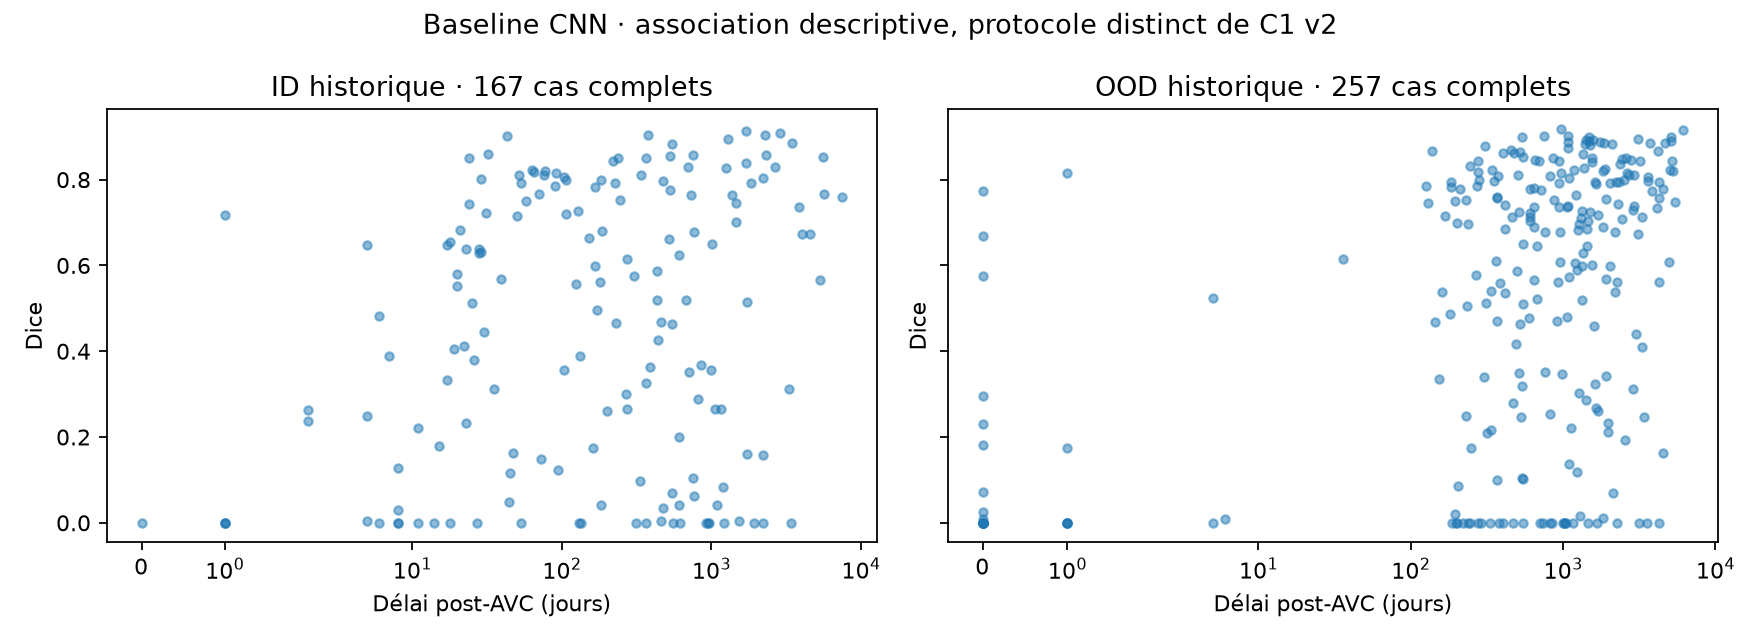
\includegraphics[width=\linewidth]{analysis/reports/s8_historical/time_dice.png}
  \caption{Dice de la baseline CNN historique selon le délai post-AVC, cas complets ID (167) et OOD (257) ; protocole distinct de C1 v2.}
  \label{fig:yosra-s8}
\end{figure}

Ces deux tests sont exploratoires, sans correction de multiplicité.
L'ID a participé au choix historique du modèle et n'est pas un test indépendant.
La partition et le prétraitement diffèrent de C1 v2.
Les résultats des autres baselines sont résumés séparément sur leurs effectifs disponibles, sans comparaison appariée implicite.

Livrables reproductibles : \nolinkurl{analysis/historical_baselines.py}, \nolinkurl{analysis/reports/s8_historical/summary.json}, \nolinkurl{README.md}, \nolinkurl{model_summary.csv}, \nolinkurl{missing_by_center.csv} et \nolinkurl{time_dice.png}.
Les empreintes des fichiers sources sont conservées.

\section{S6 : complément sur l'incertitude}
\label{sec:yosra-s6-incertitude}

Une évaluation complémentaire utilise 912 sujets d'entraînement et 228 sujets réservés, stratifiés parmi les mêmes 25 centres.
Deux classifieurs fixés, régression logistique et forêt aléatoire, sont évalués sur les mêmes sujets.
Les sujets réservés sont ensuite rééchantillonnés 10\,000 fois à l'intérieur de chaque centre, avec les mêmes indices pour toutes les représentations ; l'exactitude équilibrée donne le même poids aux centres.

Pour la forêt aléatoire, le score avant traitement (32 classes) est de 70,1~\%, avec un intervalle percentile conditionnel à 95~\% de [64,6 ; 75,5]~\%.
Après traitement (30 classes), il est de 51,1~\% [45,3 ; 57,0]~\%.
La différence appariée après moins avant est de $-19{,}0$ points [$-25{,}5$ ; $-12{,}6$].
Pour la régression logistique, elle est de $-21{,}5$ points [$-27{,}4$ ; $-15{,}5$] (\nolinkurl{analysis/reports/s6_uncertainty/intervals.csv}, \nolinkurl{analysis/reports/s6_uncertainty/paired_differences.csv}).
La variante après traitement à 150 classes est aussi rapportée pour montrer la sensibilité à la représentation, sans sélectionner uniquement le meilleur score.
La figure~\ref{fig:yosra-s6-incertitude} présente ces intervalles.

\begin{figure}[htbp]
  \centering
  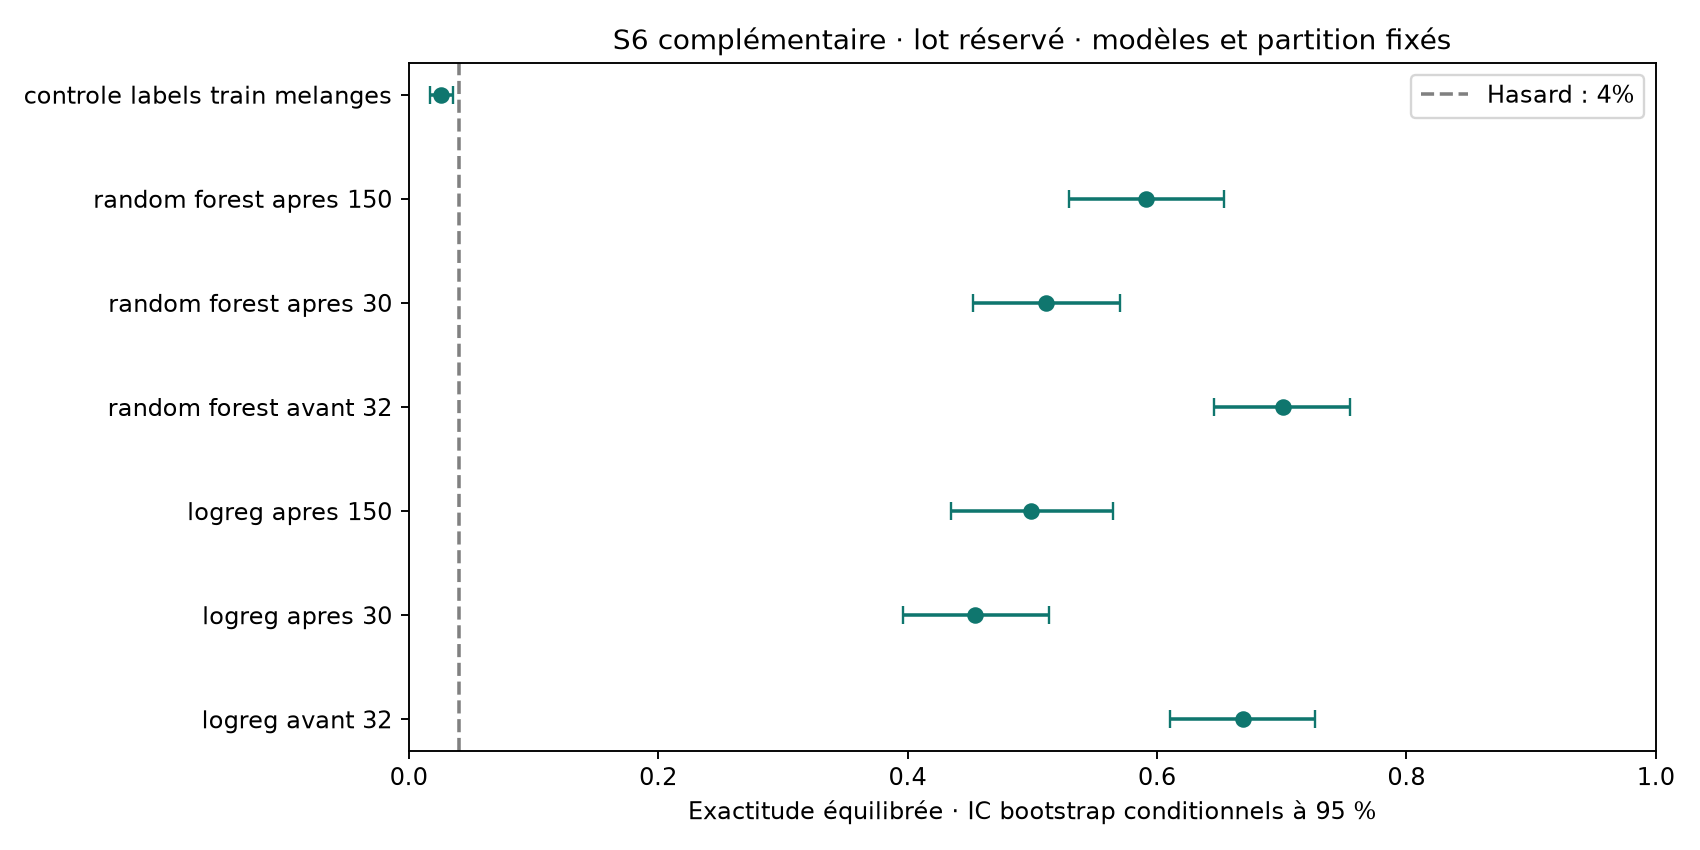
\includegraphics[width=\linewidth]{analysis/reports/s6_uncertainty/confidence_intervals.png}
  \caption{Exactitude équilibrée de la reconnaissance du centre sur le lot réservé, avec IC bootstrap conditionnels à 95~\% (modèles et partition fixés).}
  \label{fig:yosra-s6-incertitude}
\end{figure}

Ces intervalles conditionnent sur les modèles et la partition fixés : ils n'incluent pas la variabilité d'un nouvel entraînement.
La cohorte avait déjà été explorée en S6, et la granularité avant/après reste différente.
Il s'agit d'un complément exploratoire, pas d'une validation externe ni d'un effet causal isolé du prétraitement.
Les centres sont présents dans le train et le test : l'expérience mesure leur reconnaissance, pas la segmentation dans un centre inconnu.
Les moyennes des cinq plis précédentes restent inchangées et ne doivent pas être confondues avec ces nouveaux scores.

Livrables : \nolinkurl{analysis/reports/s6_uncertainty/README.md}, \nolinkurl{intervals.csv}, \nolinkurl{paired_differences.csv}, \nolinkurl{summary.json} et \nolinkurl{confidence_intervals.png}.
Les prédictions individuelles restent dans \nolinkurl{data/analysis/s6_uncertainty/} (hors du dépôt).

\section{Synthèse du contrôle qualité par centre}
\label{sec:yosra-qc}

La synthèse couvre les 1\,453 sujets inventoriés dans 55 centres.
Elle retrouve 1\,415 sujets retenus dans 54 centres, 38 exclus et aucune erreur active.
Les exclusions correspondent aux 37 cas R032 pour espacement non fiable et au cas R065 mis en quarantaine pour annotation hors du support et du recadrage.
Cette synthèse n'ajoute aucune exclusion et ne remplace pas la relecture collective des décisions.

Parmi les 1\,415 sujets retenus, cinq masques sont vides et conservés comme cas négatifs ; 1\,410 sont non vides et aucun statut de masque n'est inconnu.
Le délai post-AVC est disponible pour 1\,073 sujets ; 342 délais sont manquants ou invalides (24,2~\%).
Huit centres retenus n'ont aucun délai utilisable.
Le drapeau CHRONICITY est présent pour 296 sujets et non renseigné pour 1\,119 ; cette absence ne permet pas de déduire un stade clinique.
Deux sujets SOOP portent l'avertissement de fichier de métadonnées vide : cet avertissement de fichier ne recouvre pas toutes les valeurs de délai absentes.

Les effectifs d'exclusion utilisent tout l'inventaire ; les pourcentages de métadonnées utilisent seulement les sujets retenus de chaque centre.
Pour R032, sans sujet retenu, les taux sont non définis plutôt que nuls.
Les colonnes inconnues ne sont pas assimilées à des masques non vides.
Le tableau détaillé, la figure, les motifs d'exclusion et les avertissements sont disponibles dans \nolinkurl{analysis/reports/qc_by_center/} (\nolinkurl{summary.json}, \nolinkurl{qc_by_center.csv}, \nolinkurl{exclusion_reasons.csv}, \nolinkurl{metadata_warnings.csv}).
% La figure qc_by_center.png (55 centres sur trois panneaux) n'est pas insérée : à la largeur de la page, son texte
% ferait environ 3 pt. Elle reste disponible dans analysis/reports/qc_by_center/.
\section{Vérification de l'intégration}
\label{sec:yosra-verification}

Après la fusion des contributions de l'équipe dans \texttt{main}, 310 tests réussissent :
50 pour le pipeline et les analyses, 7 pour l'interface web, 224 pour la généralisation et
l'adaptation (dont des patchs C1 réels) et 29 pour la calibration. Quatorze tests
d'entraînement (\texttt{adaptation/tests/test\_train.py}, \texttt{test\_continual.py}) échouent
sur le Mac de vérification : \texttt{torch.amp.GradScaler} n'existe pas dans torch 2.2.2,
dernière version disponible pour macOS Intel. L'entraînement est exécuté sur Kaggle ;
l'inférence du checkpoint C8 est vérifiée localement
(\texttt{integration/reports/verification.json}).

\setlength{\emergencystretch}{0pt}
. Version LaTeX de docs/pipeline/RAPPORT.md (commit 4540d85) :
% plan, contenu et formulations conservés ; chemins des fichiers sources ajoutés pour chaque chiffre.
% Paquets attendus dans le préambule : babel (french), graphicx, booktabs, makecell, hyperref, float.
% Réglages à mettre dans le préambule du rapport final :
%   \addto\captionsfrench{\def\tablename{Tableau}}   % « Tableau » au lieu de « Table »
%   \hypersetup{hidelinks}                             % liens sans cadre rouge
% Les chemins des figures sont relatifs à la racine du dépôt.
% Statut d'origine (RAPPORT.md) : brouillon scientifique fondé sur les résultats locaux disponibles ; les valeurs
% finales doivent être prises dans les JSON/CSV générés après le dernier QC ; les expériences sans prédictions ou
% checkpoints ne sont pas présentées comme réalisées.

% Chemins de fichiers longs : coupures de ligne aussi permises après « _ » et « - » dans \nolinkurl et \url.
\makeatletter
\g@addto@macro\UrlBreaks{\do\_\do\-}
\makeatother
% Étirement d'urgence limité à ce chapitre (lignes chargées de chemins), remis à zéro à la fin.
\setlength{\emergencystretch}{3em}

\chapter{Données, décalage de domaine et démonstration}
\label{chap:yosra}

\section{Introduction et questions de recherche}
\label{sec:yosra-introduction}

Ce projet étudie la segmentation des lésions d'AVC sur des IRM T1 acquises dans plusieurs centres.
Les différences de scanner, protocole et résolution peuvent modifier la distribution des images.
Notre objectif est de mesurer ce décalage, d'évaluer la généralisation des modèles sur des centres absents de l'entraînement, puis d'étudier la possibilité d'anticiper et de réduire leur perte de performance.

Trois questions structurent le projet : quel est l'écart entre test ID et test OOD ?
Les architectures Transformer améliorent-elles la généralisation par rapport à nnU-Net ?
Quelles techniques de généralisation ou d'adaptation réduisent cet écart ?
La contribution de Yosra fournit le pipeline de données, les partitions communes, les mesures du décalage, les analyses explicatives et l'interface de démonstration.
Les comparaisons de segmentation et l'adaptation continue sont produites par Fayfa et Anas.

\section{Données et contrôle qualité}
\label{sec:yosra-donnees}

L'inventaire local contient 1\,453 paires IRM/masque dans 55 centres.
Le centre R032, soit 37 cas, est exclu provisoirement pour espacement incohérent.
Les métadonnées vides sont signalées sans supprimer une paire utilisable.
Les masques vides sont conservés comme cas négatifs.
Le délai post-AVC reste numérique ; \texttt{CHRONICITY}, codé 1/vide, n'est pas interprété comme une catégorie aigu/subaigu/chronique
(\nolinkurl{analysis/reports/qc_by_center/summary.json}, \nolinkurl{analysis/reports/qc_by_center/exclusion_reasons.csv}).

La livraison v2 contient 1\,415 volumes prétraités, relus et exportés.
Elle exclut les 37 cas R032 et met un cas supplémentaire en quarantaine technique.
Le split v1 est archivé ; v2 retire uniquement ce cas, sans déplacer les autres sujets ni les centres.
La relecture collective de cette quarantaine reste nécessaire ; les annotations brutes sont intactes
(\nolinkurl{preprocessing/reports/release_v2.json}, \nolinkurl{preprocessing/qc_exclusions.json}).

\section{Pipeline Spark}
\label{sec:yosra-pipeline}

Chaque sujet constitue une unité de travail.
Le pipeline réoriente les images en RAS, rééchantillonne à 1~mm isotrope (linéaire pour l'image, plus proche voisin pour les masques), normalise les intensités dans le support cérébral et recadre avec une marge de cinq voxels.
Le support est défini par les intensités supérieures à la valeur de fond estimée ; cette précaution traite notamment le centre R029 dont le fond n'est pas nul.
Cette heuristique reste une limite et doit être examinée sur les cas atypiques.

Le z-score est stocké en \texttt{int16} avec un pas de 0,001.
L'erreur d'arrondi est au plus 0,0005 unité de z-score.
Le validateur utilise cette borne, avec une petite marge numérique, pour la moyenne et l'écart-type ; le fond doit rester exactement nul.
Une signature des entrées et paramètres permet la reprise et chaque paire est accompagnée d'un QC (\nolinkurl{preprocessing/week4.py}).

La boîte de recadrage est déterminée par l'image seule.
Le code existant tolère la suppression de labels hors boîte jusqu'à 1~\% du volume lésionnel.
Ce choix n'est pas une correction clinique des annotations : il doit être documenté et validé.
Le dernier cas dépasse cette tolérance (1,76~\% : 77 voxels sur 4\,376, \nolinkurl{preprocessing/qc_exclusions.json}) et est mis en quarantaine dans v2.
L'option N4 a été ajoutée pour une expérience distincte ; elle n'a pas été appliquée au jeu de référence et aucun bénéfice n'en est revendiqué.

\section{Partitions et absence de fuite}
\label{sec:yosra-partitions}

Le fichier commun \nolinkurl{splits.json} version 2 fixe 916 cas d'entraînement/validation, 231 cas ID et 268 cas OOD (\nolinkurl{preprocessing/reports/release_v2.json}).
Six centres OOD sont intégralement retirés : R008, R028, R031, R034, R053 et SOOP.
Les cinq plis séparent les centres d'entraînement et de validation.
Le test ID de chaque pli est limité aux centres présents dans son entraînement.
Le découpage compte 231 sujets ID au total ; pour le pli~0, le test ID n'en garde que 185, car les 46 autres appartiennent aux centres de validation de ce pli, absents de son entraînement (\nolinkurl{splits.json}, \texttt{folds[0].id\_test}).

La sélection des centres OOD varie taille et distance d'intensité.
Comme la distance participe à cette sélection, un écart de distance ID/OOD n'est pas une découverte indépendante.
Les mesures prédictives doivent utiliser la référence d'entraînement du modèle considéré, pas le pool global.
Aucun hyperparamètre d'alerte ne doit être choisi sur le test OOD.

\section{Benchmark}
\label{sec:yosra-benchmark}

Le pilote existant porte sur huit petits volumes et un essai par configuration.
Les temps de calcul sont 56,59~s, 41,46~s, 27,63~s et 42,54~s pour 1, 2, 4 et 8 workers.
L'accélération maximale mesurée est $\times$2,05 avec quatre workers (\nolinkurl{preprocessing/reports/benchmark_summary.csv}, \nolinkurl{preprocessing/reports/benchmark_scope.json}).
La dégradation à huit workers est compatible avec des coûts de concurrence et de ressources ; ce pilote ne permet pas d'en isoler la cause.
Les workers ne constituent pas des cœurs physiques réservés.
Le démarrage Spark n'entre pas dans \texttt{compute\_seconds}.
Les courbes ne sont pas extrapolées au dataset entier.
La figure~\ref{fig:yosra-benchmark} montre l'accélération mesurée.

\begin{figure}[htbp]
  \centering
  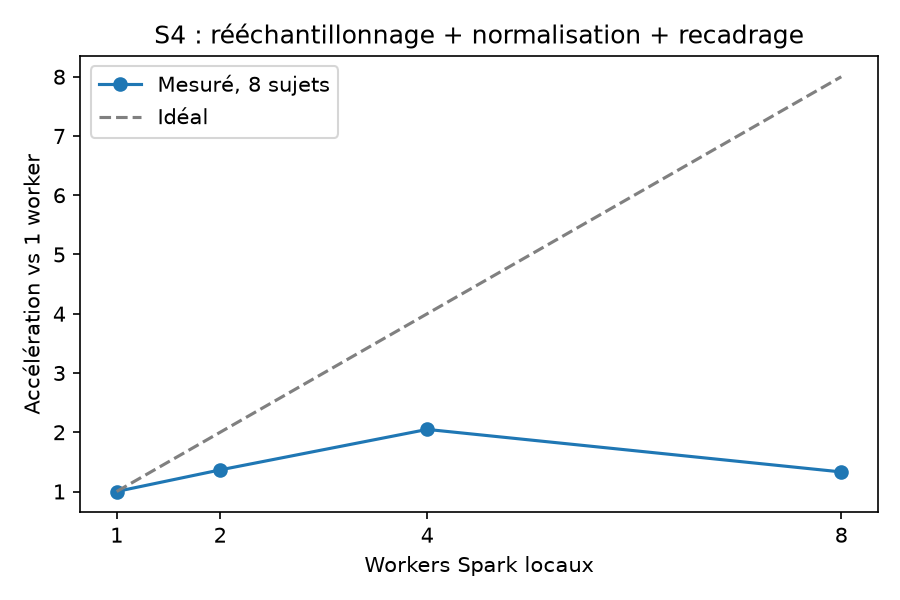
\includegraphics[width=0.6\linewidth]{preprocessing/reports/benchmark_speedup.png}
  \caption{Accélération du prétraitement S4 selon le nombre de workers Spark locaux (8 sujets, un essai).}
  \label{fig:yosra-benchmark}
\end{figure}

\section{Statistiques et empreinte du centre}
\label{sec:yosra-s5-s6}

Les rapports S5 comparent les distributions avant/après prétraitement et mesurent les distances Wasserstein et MMD entre centres et référence.
Le z-score contraint moyenne et variance par scan ; les différences restantes portent donc surtout sur la forme des distributions.
Les échelles avant/après ne sont pas identiques : leur comparaison normalisée reste descriptive.

Le test S6 prédit le centre depuis des histogrammes ou statistiques, avec cinq plis stratifiés, exactitude équilibrée et contrôle à labels mélangés.
Comparer des histogrammes de granularité proche et les mêmes patients permet de mieux isoler l'effet du prétraitement.
Une empreinte reconnaissable n'implique pas à elle seule une baisse du Dice.

Valeurs et figures : \nolinkurl{analysis/reports/post_stats_summary.json}, \nolinkurl{analysis/reports/site_fingerprint_s6.csv}, figures~\ref{fig:yosra-s5-avant-apres}, \ref{fig:yosra-s5-distances} et~\ref{fig:yosra-s6}.
Les versions historiques sur 1\,402 cas ne doivent pas être confondues avec la relance sur 1\,415.
Les versions historiques sur 1\,402 cas sont conservées dans l'historique Git du dépôt
(commit \texttt{5a86471}, fichier \texttt{analysis/reports/post\_stats\_summary.json}).

La relance du 11 novembre couvre 1\,415 sujets dans 54 centres.
La distance relative médiane passe de 0,1315 avant à 0,0376 après, sur la même cohorte disponible.
La corrélation entre Wasserstein et MMD vaut 0,842 pour les centres d'au moins cinq scans.
La médiane de Wasserstein vaut 0,0376 pour ID et 0,0900 pour OOD ; cet écart reste affecté par la sélection initiale des centres (\nolinkurl{analysis/reports/post_stats_summary.json}).
Le test S6 retient 1\,140 scans de 25 centres.
Avec les histogrammes 32 classes avant / 30 classes après et le meilleur des deux classifieurs, l'exactitude équilibrée vaut 69,7~\% puis 48,9~\%.
Le contrôle mélangé vaut 4,0~\%, proche du hasard à 4~\% (\nolinkurl{analysis/reports/site_fingerprint_s6.csv}, \nolinkurl{analysis/reports/site_fingerprint_s6_summary.json}).
Ces chiffres ne mesurent pas la performance de segmentation.

\begin{figure}[p]
  \centering
  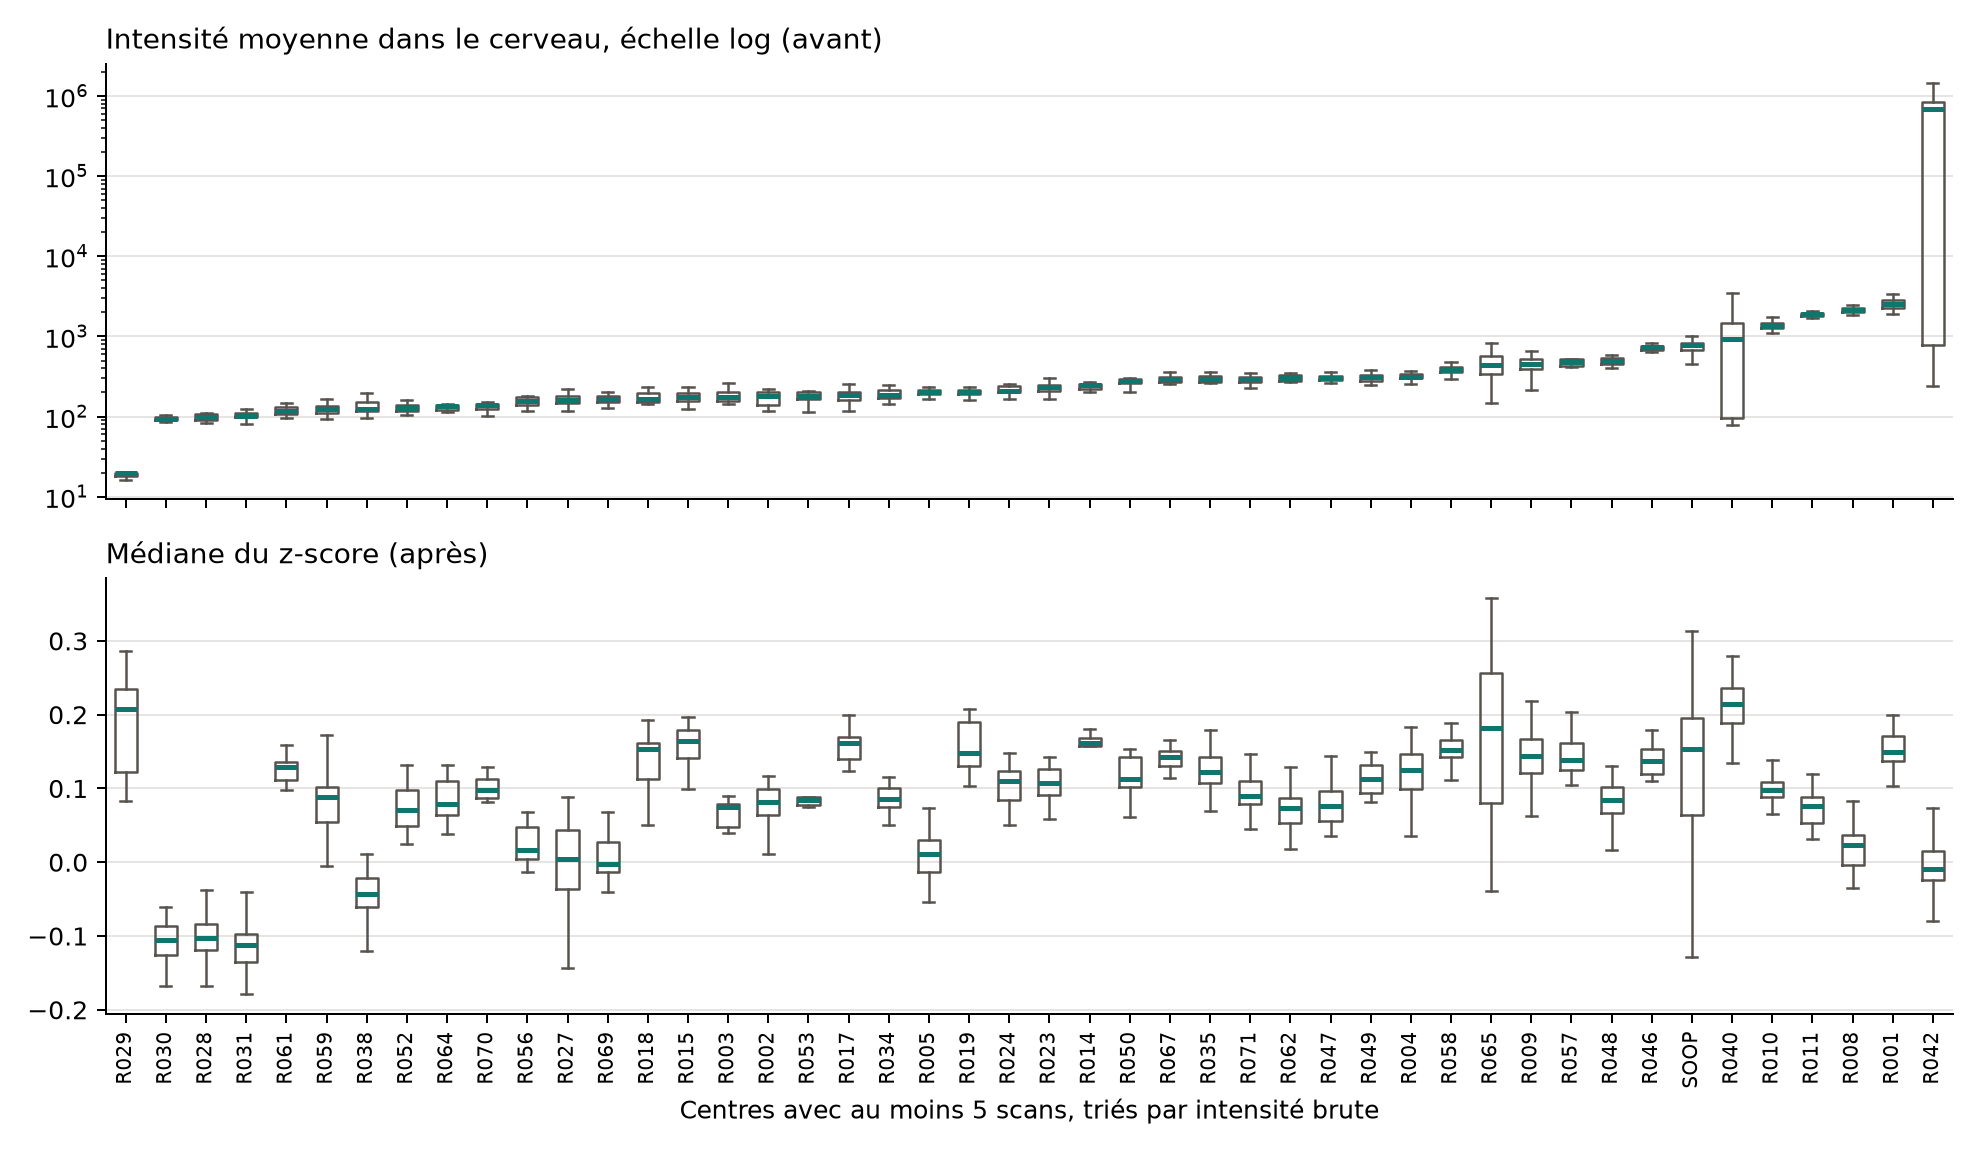
\includegraphics[angle=90,height=0.9\textheight]{figures/s5_avant_apres_par_centre.png}
  \caption{Intensité moyenne dans le cerveau avant prétraitement (échelle log) et médiane du z-score après, par centre (centres d'au moins 5 scans).}
  \label{fig:yosra-s5-avant-apres}
\end{figure}

\begin{figure}[htbp]
  \centering
  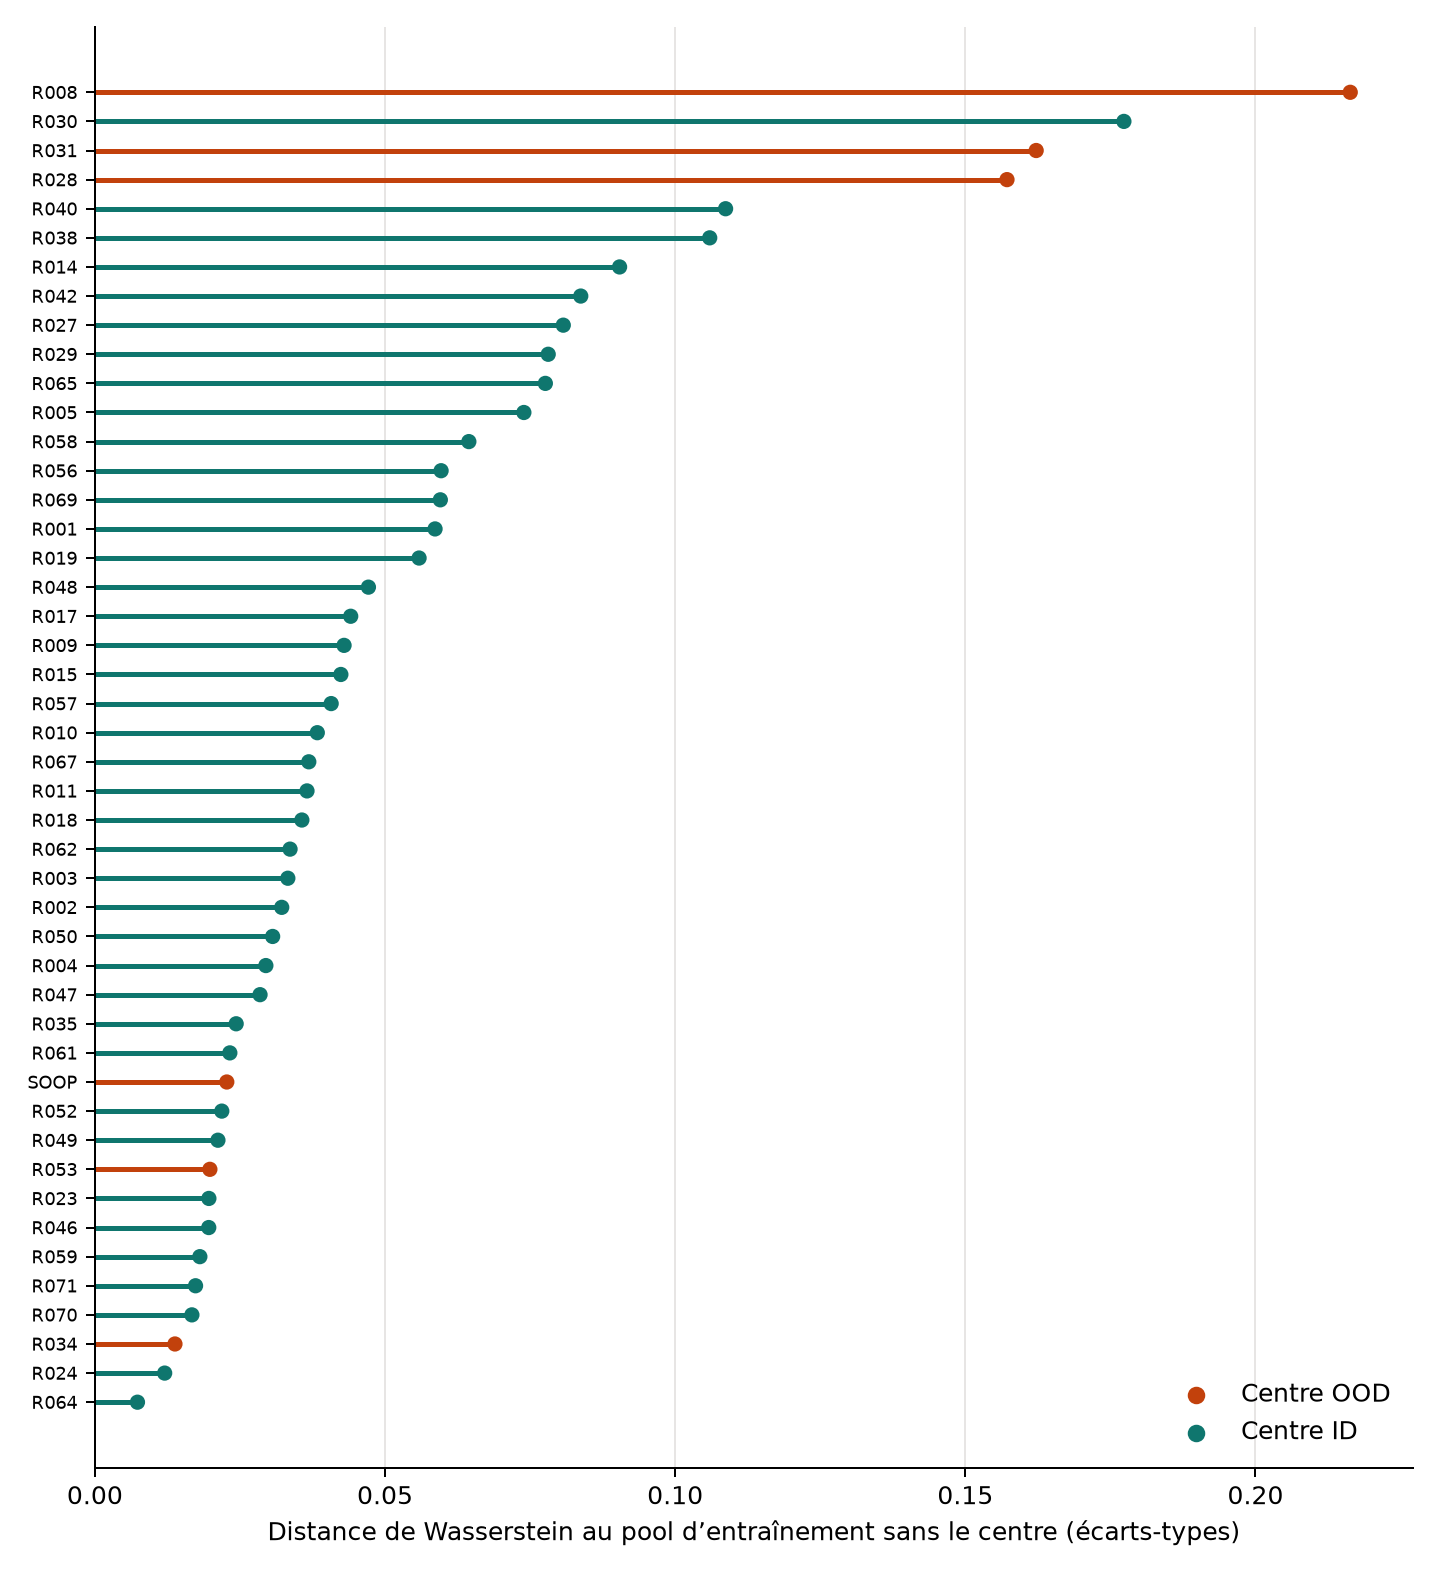
\includegraphics[width=0.85\linewidth]{figures/s5_distances_centres.png}
  \caption{Distance de Wasserstein de chaque centre au pool d'entraînement sans ce centre ; centres OOD en orange.}
  \label{fig:yosra-s5-distances}
\end{figure}

\begin{figure}[htbp]
  \centering
  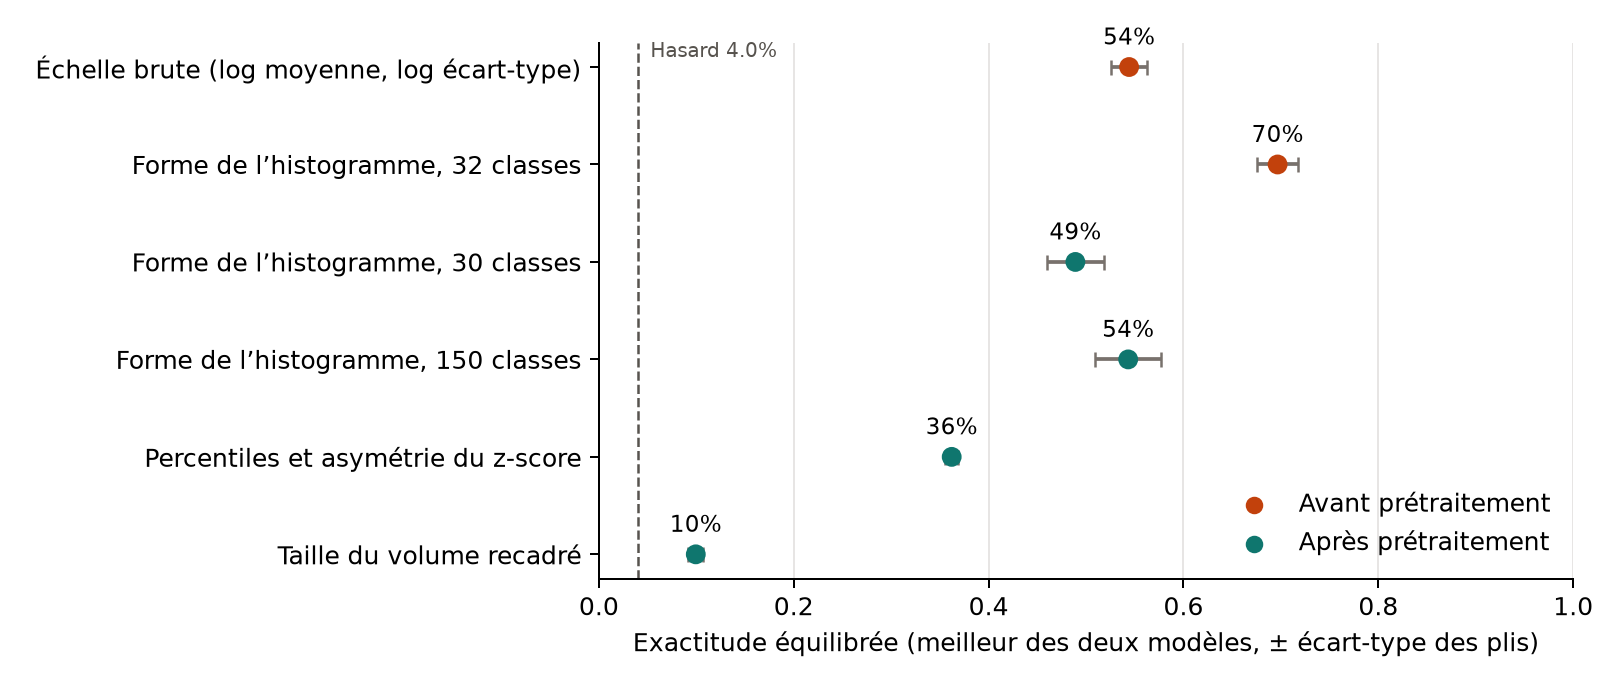
\includegraphics[width=\linewidth]{figures/s6_empreinte_centre.png}
  \caption{Empreinte du centre (S6) : exactitude équilibrée de la prédiction du centre selon la représentation, avant et après prétraitement (hasard : 4~\%).}
  \label{fig:yosra-s6}
\end{figure}

\section{Prédiction d'échec et effet du temps : protocole C1 préparé}
\label{sec:yosra-s7-s8}

S7 met en relation la distance au train du pli et l'erreur $1 - \mathrm{Dice}$ par centre.
Une validation leave-one-center-out produit des prédictions hors calibration.
La régression et le seuil d'alerte sont ajustés uniquement sur les autres centres de validation.
La différence de Dice par rapport au test ID est rapportée séparément.
Sans les résultats C3 de C1, ni corrélation empirique ni performance d'alerte ne peuvent être annoncées.

S8 compare les associations du centre et du délai post-AVC par modèles linéaires emboîtés sur les mêmes cas complets.
Le délai est transformé par $\log(1 + \textrm{jours})$.
Le test de permutation préserve le centre.
Les délais manquants, la sélection des cas et les confusions possibles limitent l'interprétation.
Le protocole n'établit pas une relation causale.

\section{Caractéristiques du réseau (C6 v2)}
\label{sec:yosra-c6}

La version C6 v2 mesure le décalage dans l'espace appris par le réseau plutôt que sur les
intensités. Le modèle C8 (U-Net 3D, augmentation d'intensité, pli 0) est gelé et utilisé en
mode évaluation, sans gradient et sans masque lésionnel. Pour chaque sujet, la sortie du
bottleneck, la couche que lit le classifieur de centre de DANN, est moyennée dans l'espace :
on obtient un vecteur de 320 valeurs par scan.
L'entrée est le volume C1 complet, complété par des zéros jusqu'à un multiple de 16. Le réseau
a été entraîné sur des patchs $96^3$ : sur le volume entier, les normalisations d'instance
portent sur une autre étendue. La même règle est appliquée à tous les scans, ce qui garde la
comparaison entre centres cohérente.

La comparaison d'empreinte baseline / augmentation / DANN demande les checkpoints baseline et
DANN du même protocole ; elle reste à faire.

\section{Démonstration et limites}
\label{sec:yosra-demo}

L'application Gradio affiche les coupes d'une IRM et un masque, calcule le volume lésionnel en mL et accepte une carte d'incertitude.
Un adaptateur permet de brancher le modèle final.
NiiVue fournit une vue 3D locale sur la route \texttt{/viewer/} du même serveur.
ANTsPy peut recaler un template MNI et transférer un atlas de labels ; une inspection visuelle demeure nécessaire avant de nommer les régions.

L'alerte individuelle d'intensité utilise un quantile de validation distinct du seuil par centre.
Elle n'est ni une garantie de performance ni une décision clinique.
En l'absence d'une entrée requise, l'application indique ce qui manque au lieu de créer un résultat.
Le support animé de secours est synthétique et explicitement étiqueté.

\subsection{Interface web du projet}
\label{sec:yosra-frontend}

Une application web (\texttt{frontend/}) présente l'ensemble du projet en dix pages :
vue d'ensemble, avancement du pipeline, contrôle qualité, prétraitement Spark, décalage entre
centres, modèles et Dice, adaptation de domaine, démonstration IRM avec vue 3D, conclusions
et galerie des figures. Le serveur FastAPI lit uniquement les rapports versionnés du dépôt
(\texttt{analysis/reports}, \texttt{preprocessing/reports}, \texttt{baselines/outputs},
\texttt{adaptation/outputs}, \texttt{integration/reports}) : aucun chiffre n'est simulé, et une
expérience absente est signalée comme telle. Chaque page et chaque carte indiquent qui a
produit le résultat. L'interface fonctionne sans étape de construction ni ressource externe ;
seules les figures des dossiers de résultats sont servies, jamais les données IRM. Sept tests
couvrent l'API (\texttt{frontend/tests/test\_server.py}).

\subsection{Branchement du modèle C8}
\label{sec:yosra-c8}

La démonstration (\texttt{demo/app.py}) et l'interface web appellent la fonction désignée par
la variable \texttt{AVC\_PREDICT\_ADAPTER}, au format \texttt{module:fonction}. L'adaptateur de
l'équipe, \texttt{adaptation.demo\_adapter:predict}, applique le prétraitement S4 puis le modèle
retenu (augmentation d'intensité, pli 0) et enregistre le masque en NIfTI \texttt{uint8} dans la
grille de l'IRM reçue. Il demande PyTorch et MONAI, absents de l'environnement de la
démonstration. Le pont \texttt{demo/c8\_bridge.py} lance donc cet adaptateur dans
l'environnement du modèle, dans un processus séparé, et récupère le masque ; la démonstration
utilise \texttt{AVC\_PREDICT\_ADAPTER=c8\_bridge:predict}. Le checkpoint est lu dans
\texttt{data/modeles/unet3d\_intensity\_pli0\_best.pt} (SHA-256 \texttt{ee6b93af\ldots abb6}),
hors du dépôt.

Sur le sujet OOD R034\_sub-r034s003\_ses-1, le rapport de la démonstration donne un volume
lésionnel de 27,058~mL (27\,058 voxels de 1~mm$^3$). Cette valeur concorde avec le volume
prédit lors de l'évaluation du modèle : 27,054~mL dans le fichier \texttt{resultats\_ood\_test.csv}
de la run intensité, conservé hors du dépôt. Sur le sujet OOD R031\_sub-r031s006\_ses-1, envoyé
sans masque à l'interface web, le modèle prédit 33,8~mL pour 27,7~mL annotés, soit un Dice de
0,745, en environ 35~s sur processeur. Ces deux cas vérifient le branchement ; ils ne constituent
pas une évaluation. Le modèle ne produit pas de carte d'incertitude. Cinq tests couvrent les
erreurs du pont (\texttt{tests/test\_c8\_bridge.py}).

\section{Discussion et travaux à terminer}
\label{sec:yosra-discussion}

Les principales limites actuelles sont la quarantaine QC à relire collectivement, le faible nombre de centres pour calibrer un prédicteur d'échec, la dépendance des distances aux effectifs, les métadonnées manquantes et l'absence locale des checkpoints et des Dice correspondant à C1 v2.
Les résultats RQ3 du pli 0 et le checkpoint C8 sont désormais disponibles (chapitre RQ3,
conclusion). Les analyses S7 et S8 sur C1 v2 attendent encore les Dice par sujet, y compris
sur la validation, qui sert à calibrer le seuil d'alerte sans consulter le test. L'empreinte
avant/après DANN attend les checkpoints baseline et DANN. La vidéo de vraie inférence et la
relecture collective restent à faire.
Une analyse S8 historique distincte est disponible plus bas (section~\ref{sec:yosra-s8-historique}).
Les références bibliographiques du document de projet doivent être vérifiées dans leurs publications originales avant d'être reprises dans la version remise.

\section{Compléments vérifiés de la livraison v2}
\label{sec:yosra-livraison}

L'export nnU-Net contient 916 images et labels d'entraînement, 499 images de test (231 ID, 268 OOD) et cinq plis (\nolinkurl{preprocessing/reports/export_v2.json}).
Le contrôle officiel nnU-Net reste à lancer dans l'environnement d'entraînement de Fayfa.
Les autres appartenances de v1 sont conservées.

L'analyse descriptive S8 trouve 1\,073 délais utilisables et 342 manquants ou invalides ; le délai médian est de 365 jours.
Huit centres n'ont aucun délai utilisable.
L'association centre / log-délai (eta carré 0,7475) souligne la nécessité de tenir compte du centre ; elle ne mesure pas l'effet du délai sur le Dice.
Voir \nolinkurl{analysis/reports/s8_metadata/} (\nolinkurl{summary.json}).

Le seuil individuel d'atypie du pli~0 vaut 0,114885 : référence de 733 scans du train, quantile 95~\% sur 183 scans de validation.
Aucun test ID/OOD n'a servi à ce réglage.
Le seuil est enregistré dans \texttt{data/demo/reference\_ood.json} (pli 0, quantile 0,95,
733 scans d'entraînement, 183 de validation), hors du dépôt comme l'ensemble de \texttt{data/}.

Chrome a chargé l'application, produit le rapport synthétique de 2,091~mL, puis affiché les coupes et le rendu 3D NiiVue sans erreur JavaScript (\nolinkurl{docs/pipeline/demo_verification/browser_report.json}).
L'image Docker a été construite et ses routes ainsi que le calcul du rapport ont été testés (\nolinkurl{docs/pipeline/verification.json}).
La vidéo de secours MP4 utilise ces captures réelles d'interface sur un phantom explicitement synthétique ; elle ne montre pas une inférence du réseau.

L'atlas Harvard-Oxford et le template compatible MNI152NLin6Asym ont été récupérés avec leurs sources et empreintes dans \nolinkurl{data/demo/atlas/provenance.json} (hors du dépôt ; copie versionnée : \nolinkurl{docs/pipeline/demo_verification/atlas_provenance.json}).
Les labels corticaux sont prioritaires, puis les labels sous-corticaux décalés de 100 ; les zones non couvertes gardent la valeur zéro.
Le recalage natif exige une relecture anatomique.
Sources : Nilearn Harvard-Oxford\footnote{\url{https://nilearn.github.io/stable/modules/generated/nilearn.datasets.fetch_atlas_harvard_oxford.html}} et TemplateFlow MNI152NLin6Asym\footnote{\url{https://github.com/templateflow/tpl-MNI152NLin6Asym}}.

Le recalage SyN sur l'exemple réel a été exécuté.
Atlas et IRM ont la même grille, les labels restent entiers et 97,75~\% des voxels atlas non nuls se trouvent dans le support d'intensité de l'image (\nolinkurl{docs/pipeline/verification.json}).
La planche locale \nolinkurl{data/demo/registration/qc_overlay.png} (hors du dépôt) a été examinée dans trois plans ; cela ne remplace pas une relecture anatomique experte.
Le rapport régional utilise le masque de référence fourni, sans inférence de réseau.

\section{S8 : résultat exploratoire sur les baselines récupérées}
\label{sec:yosra-s8-historique}

Le 12 novembre, les scores historiques de \texttt{cnn\_pretrained\_freeze-none} ont été rattachés à leur propre partition (903 train, 226 ID validation, 287 OOD), sans les reclasser dans C1 v2.
L'analyse utilise 167 cas ID complets de 31 centres et 257 cas OOD de 12 centres.
En ID, 58 délais manquent ou sont invalides et un Dice est absent ; en OOD, 30 délais manquent ou sont invalides.
Le Dice absent du cas à masque vide n'est pas remplacé par un score supposé.

Après ajustement sur le centre, l'ajout de $\log(1 + \textrm{délai})$ augmente le R$^2$ de 0,000046 en ID ($p$ exploratoire $= 0{,}911$) et de 0,03808 en OOD ($p = 0{,}001$ ; 999 permutations intra-centre pour chaque groupe).
Après ajout de $\log(1 + \textrm{volume lésionnel})$, ces gains sont respectivement 0,000711 et 0,000217 (\nolinkurl{analysis/reports/s8_historical/summary.json}).
L'association OOD dépend donc fortement des variables prises en compte ; elle ne permet pas d'attribuer un effet causal au temps.
Le volume est une analyse de sensibilité, pas un ajustement causal validé.
La figure~\ref{fig:yosra-s8} montre les cas utilisés.

\begin{figure}[htbp]
  \centering
  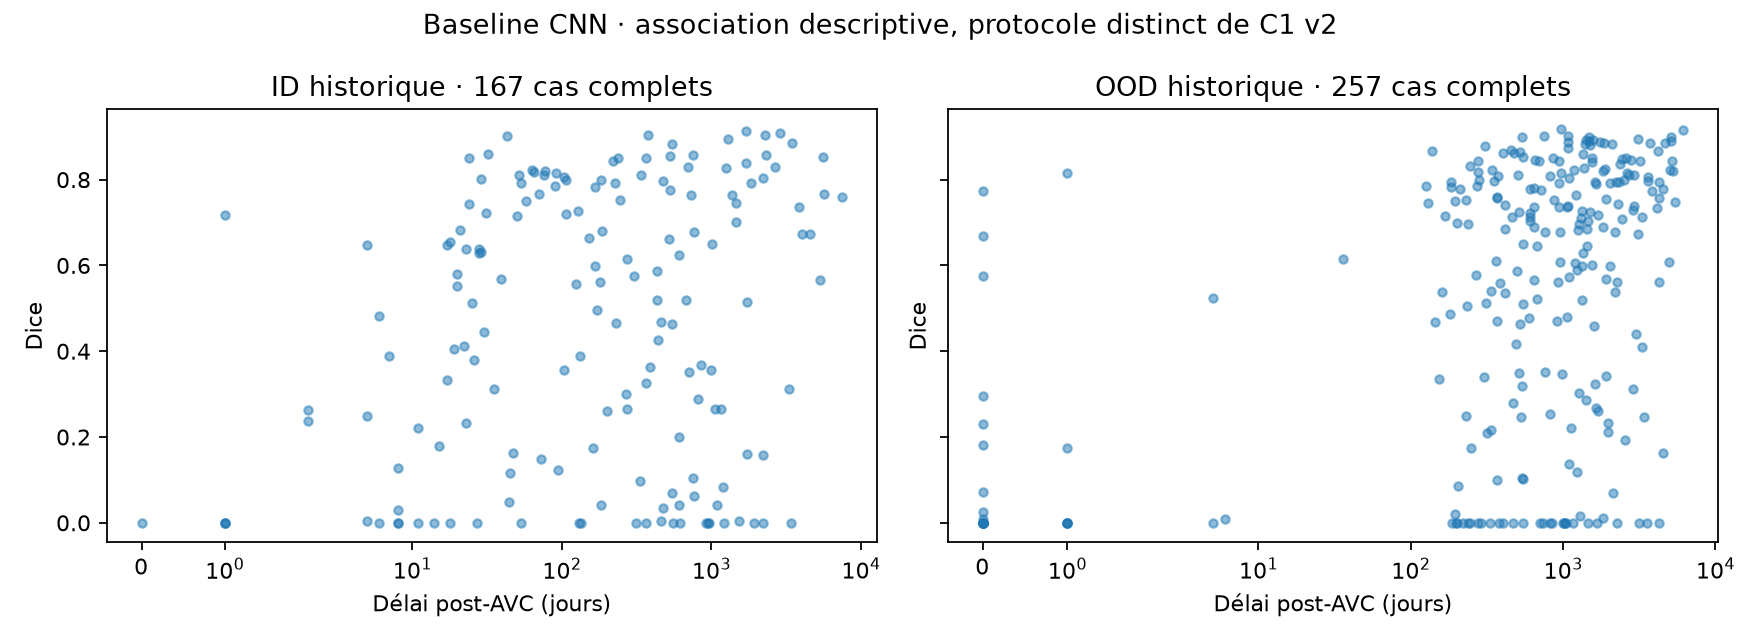
\includegraphics[width=\linewidth]{analysis/reports/s8_historical/time_dice.png}
  \caption{Dice de la baseline CNN historique selon le délai post-AVC, cas complets ID (167) et OOD (257) ; protocole distinct de C1 v2.}
  \label{fig:yosra-s8}
\end{figure}

Ces deux tests sont exploratoires, sans correction de multiplicité.
L'ID a participé au choix historique du modèle et n'est pas un test indépendant.
La partition et le prétraitement diffèrent de C1 v2.
Les résultats des autres baselines sont résumés séparément sur leurs effectifs disponibles, sans comparaison appariée implicite.

Livrables reproductibles : \nolinkurl{analysis/historical_baselines.py}, \nolinkurl{analysis/reports/s8_historical/summary.json}, \nolinkurl{README.md}, \nolinkurl{model_summary.csv}, \nolinkurl{missing_by_center.csv} et \nolinkurl{time_dice.png}.
Les empreintes des fichiers sources sont conservées.

\section{S6 : complément sur l'incertitude}
\label{sec:yosra-s6-incertitude}

Une évaluation complémentaire utilise 912 sujets d'entraînement et 228 sujets réservés, stratifiés parmi les mêmes 25 centres.
Deux classifieurs fixés, régression logistique et forêt aléatoire, sont évalués sur les mêmes sujets.
Les sujets réservés sont ensuite rééchantillonnés 10\,000 fois à l'intérieur de chaque centre, avec les mêmes indices pour toutes les représentations ; l'exactitude équilibrée donne le même poids aux centres.

Pour la forêt aléatoire, le score avant traitement (32 classes) est de 70,1~\%, avec un intervalle percentile conditionnel à 95~\% de [64,6 ; 75,5]~\%.
Après traitement (30 classes), il est de 51,1~\% [45,3 ; 57,0]~\%.
La différence appariée après moins avant est de $-19{,}0$ points [$-25{,}5$ ; $-12{,}6$].
Pour la régression logistique, elle est de $-21{,}5$ points [$-27{,}4$ ; $-15{,}5$] (\nolinkurl{analysis/reports/s6_uncertainty/intervals.csv}, \nolinkurl{analysis/reports/s6_uncertainty/paired_differences.csv}).
La variante après traitement à 150 classes est aussi rapportée pour montrer la sensibilité à la représentation, sans sélectionner uniquement le meilleur score.
La figure~\ref{fig:yosra-s6-incertitude} présente ces intervalles.

\begin{figure}[htbp]
  \centering
  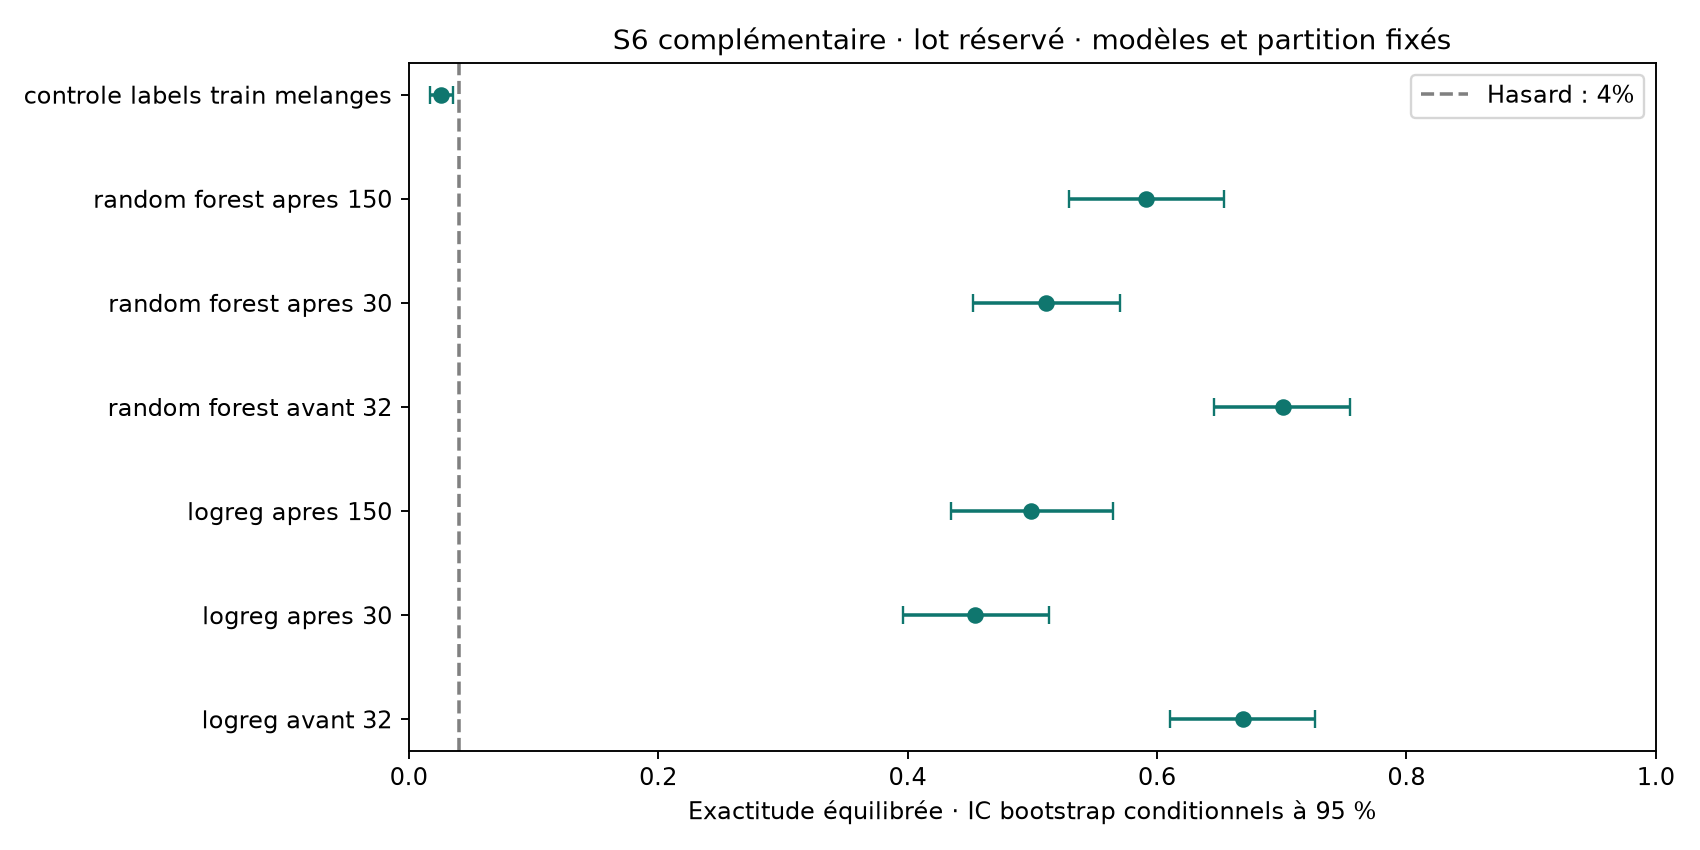
\includegraphics[width=\linewidth]{analysis/reports/s6_uncertainty/confidence_intervals.png}
  \caption{Exactitude équilibrée de la reconnaissance du centre sur le lot réservé, avec IC bootstrap conditionnels à 95~\% (modèles et partition fixés).}
  \label{fig:yosra-s6-incertitude}
\end{figure}

Ces intervalles conditionnent sur les modèles et la partition fixés : ils n'incluent pas la variabilité d'un nouvel entraînement.
La cohorte avait déjà été explorée en S6, et la granularité avant/après reste différente.
Il s'agit d'un complément exploratoire, pas d'une validation externe ni d'un effet causal isolé du prétraitement.
Les centres sont présents dans le train et le test : l'expérience mesure leur reconnaissance, pas la segmentation dans un centre inconnu.
Les moyennes des cinq plis précédentes restent inchangées et ne doivent pas être confondues avec ces nouveaux scores.

Livrables : \nolinkurl{analysis/reports/s6_uncertainty/README.md}, \nolinkurl{intervals.csv}, \nolinkurl{paired_differences.csv}, \nolinkurl{summary.json} et \nolinkurl{confidence_intervals.png}.
Les prédictions individuelles restent dans \nolinkurl{data/analysis/s6_uncertainty/} (hors du dépôt).

\section{Synthèse du contrôle qualité par centre}
\label{sec:yosra-qc}

La synthèse couvre les 1\,453 sujets inventoriés dans 55 centres.
Elle retrouve 1\,415 sujets retenus dans 54 centres, 38 exclus et aucune erreur active.
Les exclusions correspondent aux 37 cas R032 pour espacement non fiable et au cas R065 mis en quarantaine pour annotation hors du support et du recadrage.
Cette synthèse n'ajoute aucune exclusion et ne remplace pas la relecture collective des décisions.

Parmi les 1\,415 sujets retenus, cinq masques sont vides et conservés comme cas négatifs ; 1\,410 sont non vides et aucun statut de masque n'est inconnu.
Le délai post-AVC est disponible pour 1\,073 sujets ; 342 délais sont manquants ou invalides (24,2~\%).
Huit centres retenus n'ont aucun délai utilisable.
Le drapeau CHRONICITY est présent pour 296 sujets et non renseigné pour 1\,119 ; cette absence ne permet pas de déduire un stade clinique.
Deux sujets SOOP portent l'avertissement de fichier de métadonnées vide : cet avertissement de fichier ne recouvre pas toutes les valeurs de délai absentes.

Les effectifs d'exclusion utilisent tout l'inventaire ; les pourcentages de métadonnées utilisent seulement les sujets retenus de chaque centre.
Pour R032, sans sujet retenu, les taux sont non définis plutôt que nuls.
Les colonnes inconnues ne sont pas assimilées à des masques non vides.
Le tableau détaillé, la figure, les motifs d'exclusion et les avertissements sont disponibles dans \nolinkurl{analysis/reports/qc_by_center/} (\nolinkurl{summary.json}, \nolinkurl{qc_by_center.csv}, \nolinkurl{exclusion_reasons.csv}, \nolinkurl{metadata_warnings.csv}).
% La figure qc_by_center.png (55 centres sur trois panneaux) n'est pas insérée : à la largeur de la page, son texte
% ferait environ 3 pt. Elle reste disponible dans analysis/reports/qc_by_center/.
\section{Vérification de l'intégration}
\label{sec:yosra-verification}

Après la fusion des contributions de l'équipe dans \texttt{main}, 310 tests réussissent :
50 pour le pipeline et les analyses, 7 pour l'interface web, 224 pour la généralisation et
l'adaptation (dont des patchs C1 réels) et 29 pour la calibration. Quatorze tests
d'entraînement (\texttt{adaptation/tests/test\_train.py}, \texttt{test\_continual.py}) échouent
sur le Mac de vérification : \texttt{torch.amp.GradScaler} n'existe pas dans torch 2.2.2,
dernière version disponible pour macOS Intel. L'entraînement est exécuté sur Kaggle ;
l'inférence du checkpoint C8 est vérifiée localement
(\texttt{integration/reports/verification.json}).

\setlength{\emergencystretch}{0pt}
